\documentclass[8pt]{beamer}

%%pacotes referentes ao Beamer
%\useoutertheme{split}
%\setbeamertemplate{navigation symbols}{}

%\usetheme{beamertheme}
%\usebeamercolor{beamer-color name}

%\usetheme{Boadilla}
%\usecolortheme{dove}

\usetheme{Montpellier}
\usecolortheme{beaver}

% \usetheme{pittsburgh}
% \usecolortheme{dolphin}
%\usecolortheme{dove}
%\usecolortheme{seahorse}

%\usetheme{Montpellier}

%number in figures an tables -- beamer
\setbeamertemplate{caption}[numbered]

%Colocar no description
%[leftmargin=!,labelwidth=\widthof{Turma A}]
	
%pacotes usuais do latex
\usepackage[portuguese]{babel}
\usepackage[utf8]{inputenc}
\usepackage{bm}
\usepackage{graphicx}
\usepackage{subfig}
\usepackage[round]{natbib}
\usepackage{tikz}
\usetikzlibrary{shapes,arrows}
\usepackage{natbib}
\usepackage{times}
\usepackage{calc} %computes the length of a string
\usepackage{dsfont} %pacote para o 1 estilisado para indicadora
\usepackage{enumerate} %permite fazer uns enumerates diferentes
\usepackage[font=small,labelfont=bf]{caption} %permite colocar um segundo caption
\usepackage{booktabs} % comando \toprule, \midrule e \bottomrule
\usepackage{times} %times new roman font
\usepackage{multirow} %comando \multirow
\usepackage{setspace}
\usepackage{xcolor} %texto colorido
\usepackage{booktabs} %costumized tabs
\usepackage{physics} %absolute value
\usepackage{xcolor}
\usepackage{ulem}


\usepackage{listings}

\definecolor{codegreen}{rgb}{0,0.6,0}
\definecolor{codegray}{rgb}{0.5,0.5,0.5}
\definecolor{codepurple}{rgb}{0.58,0,0.82}
\definecolor{backcolour}{rgb}{0.95,0.95,0.92}

\lstdefinestyle{mystyle}{
	backgroundcolor=\color{backcolour},   
	commentstyle=\color{codegreen},
	numberstyle=\tiny\color{codegray},
	stringstyle=\color{codepurple},
	basicstyle=\ttfamily\footnotesize,
	breakatwhitespace=false,         
	breaklines=true,                 
	captionpos=b,                    
	keepspaces=true,                 
	numbers=left,                    
	numbersep=5pt,                  
	showspaces=false,                
	showstringspaces=false,
	showtabs=false,                  
	tabsize=2
}

\lstset{style=mystyle}

\renewcommand{\lstlistingname}{Código}% Listing -> Código
\renewcommand{\lstlistlistingname}{Lista de \lstlistingname s}% List of Listings -> List of Código

\usepackage{etoolbox}% http://ctan.org/pkg/etoolbox
\AtBeginEnvironment{figure}{\setcounter{subfigure}{0}}% Resets subfigure counter at start of figure environment

% my own color
\definecolor{important}{RGB}{0,153,0}




%código para alinhar a esquerda os itens no description
\defbeamertemplate{description item}{align left}{\insertdescriptionitem\hfill}
\defbeamertemplate{enumerate item}{align left}{\insertdescriptionitem\hfill}



%AMS packages
\usepackage{amsmath}
\usepackage{amsfonts}
\usepackage{amssymb}

%Não quebre linhas
\binoppenalty=\maxdimen
\relpenalty=\maxdimen

%Comandos criados por mim
\DeclareMathOperator*{\argmin}{arg\,min}

\DeclareMathOperator*{\argmax}{arg\,max}


\DeclareMathOperator{\espe}{E}

\DeclareMathOperator{\spann}{span}

\DeclareMathOperator{\cov}{Cov}

\DeclareMathOperator{\vari}{Var}

%Informações para o primeiro slide
\date{}
\title[Teste de Hipóteses]{Introdução ao teste de hipóteses}
\author[Gilberto Sassi]{Gilberto Pereira Sassi}
\institute[IME -- UFBA]{Universidade Federal da Bahia \\ Instituto de Matem\'{a}tica e Estat\'{i}stica\\ Departamento de Estat\'{i}stica }

\begin{document}
	
\tikzstyle{decision} = [diamond, draw, fill=blue!20, 
text width=4.5em, text badly centered, node distance=3cm, inner sep=0pt]
\tikzstyle{block} = [rectangle, draw, fill=blue!20, 
text width=5em, text centered, rounded corners, minimum height=4em]
\tikzstyle{line} = [draw, -latex]
\tikzstyle{cloud} = [draw, ellipse,fill=red!20, node distance=3cm,
minimum height=2em]
	
\begin{frame}{}
	\maketitle
\end{frame}

\section{Introdução}

\subsection{Conceitos iniciais}

\begin{frame}{Conceito iniciais}

\small

 \begin{block}{Objetivo}
 \begin{itemize}
  \item Decidir entre $H_0$ e $H_1$ usando as evidências presentes na amostra (tomando a melhor decisão possível ou decisão ótima usando as informações presentes na amostra);
  \item $H_0$ e $H_1$ são hipóteses complementares, ou seja, a negação da hipótese $H_0$ é $H_1$;
  \item $H_0$ e $H_1$ são declarações sobre um parâmetro (ou vários parâmetros) de uma populações (ou duas ou mais populações);
  \item $H_0$ é chamada de hipótese nula;
  \item $H_1$é chamada de hipótese alternativa.
 \end{itemize}
 \end{block}

 Observe que podemos tomar duas decisões erradas:
 \begin{enumerate}[i.]
  \item \textbf{Erro tipo I:} Aceitar $H_1$ quando $H_0$ é verdadeira, ou seja, rejeitar $H_0$ quando $H_0$ é verdadeira;
  \item \textbf{Erro tipo II:} Aceitar $H_0$ quando $H_1$ é verdadeira, ou seja, não rejeitar $H_0$ quando $H_1$ é verdadeira;
 \end{enumerate}

 \begin{table}[ht]
  \centering
  \caption{Erro tipo I e II.}
  \scalebox{0.7}{
  \begin{tabular}{|l|l|c|c|}
  \toprule[0.05cm]
  \multicolumn{2}{|c}{}& \multicolumn{2}{c|}{Situação na população}\\ \cmidrule{3-4}
  \multicolumn{2}{|c}{} & $H_0$ & $H_1$ (Negação de $H_0$)\\ \cmidrule{3-4}
  \multirow{2}{*}{Decisão} &$H_0$ & Sem erro (verdadeiro negativo) & Erro tipo II (Falso negativo) \\
  &$H_1$ (Negação de $H_0$) & Erro tipo I (Falso positivo) & Sem erro (Verdadeiro positivo)\\
  \bottomrule[0.05cm]
  \end{tabular}
	}
 \end{table}
\normalsize

\end{frame}

\begin{frame}{Conceitos iniciais}

\scriptsize

\begin{block}{Uso mais comuns}
	\begin{itemize}
		\item Verificar se o parâmetro mudou de valor em um novo cenário;
		\item Validar uma teoria ou modelo;
		\item Checar especificações (valor padrão estabelecido do mercado ou valor estabelecido por um  regulador);
	\end{itemize}
\end{block}
\vfill

\begin{block}{Roteiro para especificar as hipóteses}
	\begin{itemize}
		\item \textcolor{important}{Coloque em $H_0$ o valor padrão ou o valor padrão de mercado ou valor especificado por órgão regulador;}
		\item \textcolor{important}{Coloque em $H_1$ sua hipótese de pesquisa};
		\item \textbf{Dica:} Na dúvida, pense que a igualdade sempre vai na hipótese nula por construção da regra decisão entre $H_0$ e $H_1$.
	\end{itemize}	 
\end{block}

\begin{block}{Notação}
	\textcolor{important}{O erro com a consequência mais grave geralmente indica quem será o $H_1$ (falso positivo é mais grave)}, pois controlamos $P(\mbox{Decidir por }H_1 \mid H_0\mbox{ é verdadeira})$.

	\textbf{Exemplo:} Em um julgamento, temos as seguintes hipóteses,
	\begin{itemize}
		\item $H_0:$ réu é inocente. (Se não tem certeza da culpa, declare inocência);
		\item $H_1:$ réu  é culpada. (Precisa ser uma decisão com muita certeza).
	\end{itemize}
	Em um julgamento, o juiz decidi por $H_1$ se tivermos provas robustas e convincentes. Se não existir provas, o juiz não pode decidir por $H_1$ e ele conclui por $H_0$ por falta de evidência \sout{mas o réu pode ser culpado, você apenas não conseguiu provas e decisão por $H_0$ é ``mais fraca''}.
	
	Neste contexto, usamos a seguinte notação:
	\begin{itemize}
		\item ``Decisão por $H_0$'': não rejeitamos $H_0$ \sout{Não rejeitamos a inocência do réu};
		\item ``Decisão por $H_1$'': rejeitamos $H_0$ \sout{Rejeitamos a inocência do réu}. (Rejeitamos $H_0$ apenas se tivermos forte evidência).
	\end{itemize}
\end{block}

\normalsize

\end{frame}

\begin{frame}{Exemplo de motivação. (Procedimento de Neyman-Pearson)}

\large

Imagine que no ano de 2017, $10.000$ alunos das universidades federais cursaram ``Estatística Básica''. No ano de 2016, a nota final média dos alunos foi $5$ e queremos decidir entre duas hipóteses 
\begin{description}
  \item[$H_0$:]  A nota final em $2017$ permaneceu a mesma de $2016(\mu=5)$;
  \item[$H_1$:]  A nota final em $2017$ foi diferente de $2016(\mu\neq 5)$.
\end{description}
\vfill

Descobrir a nota de 10.000 alunos pode ser difícil, então podemos escolher aleatoriamente 1.000 alunos e precisamos decidir entre $H_0$ e $H_1$.
\vfill
  
Imagine três amostras distintas:
\begin{description}
\item[Amostra A:] nota média na amostra A é 2,5;  
\item[Amostra B:] nota média na amostra A é 5; 
\item[Amostra C:] nota média na amostra A é 7,5;
\end{description}

\normalsize

\end{frame}

\begin{frame}{Exemplo de motivação (Procedimento de Neyman-Pearson)}
\begin{figure}
\centering
\subfloat[Amostra A]{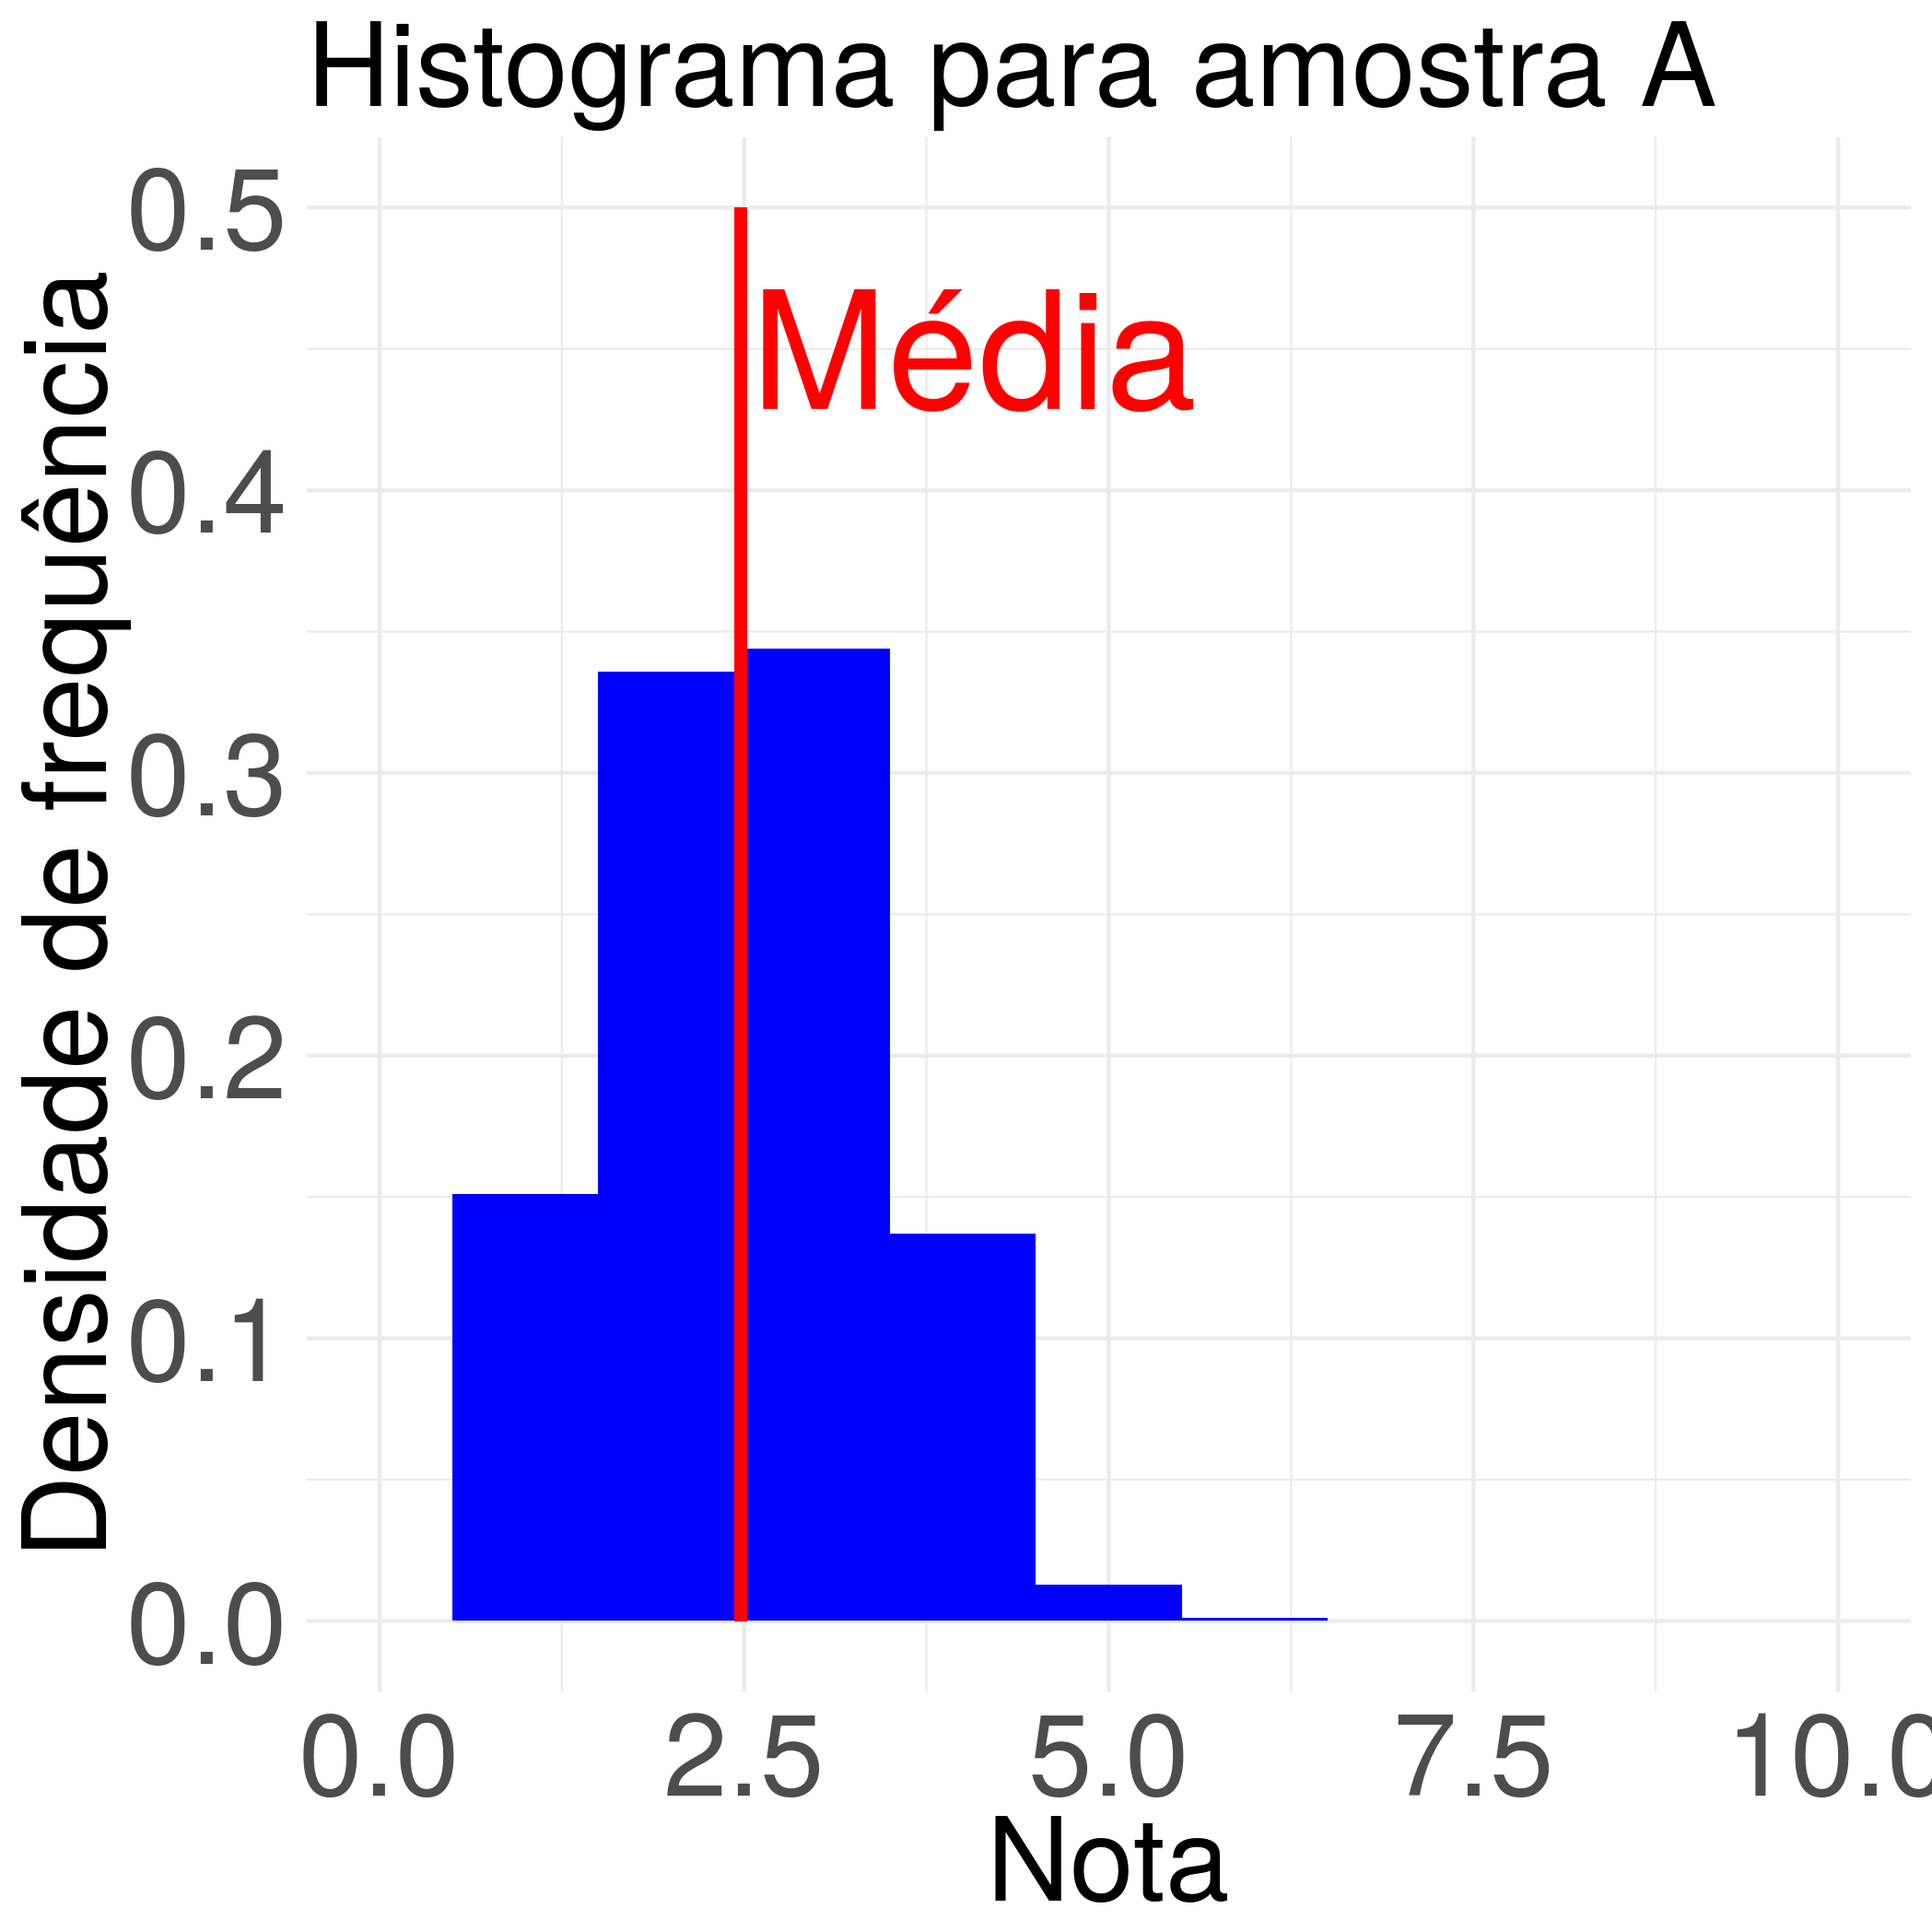
\includegraphics[width=.275\linewidth]{figures/histograma_amostra_a.png}\label{fig:amostra_a}} \hspace{0.15\linewidth}
\subfloat[Amostra B]{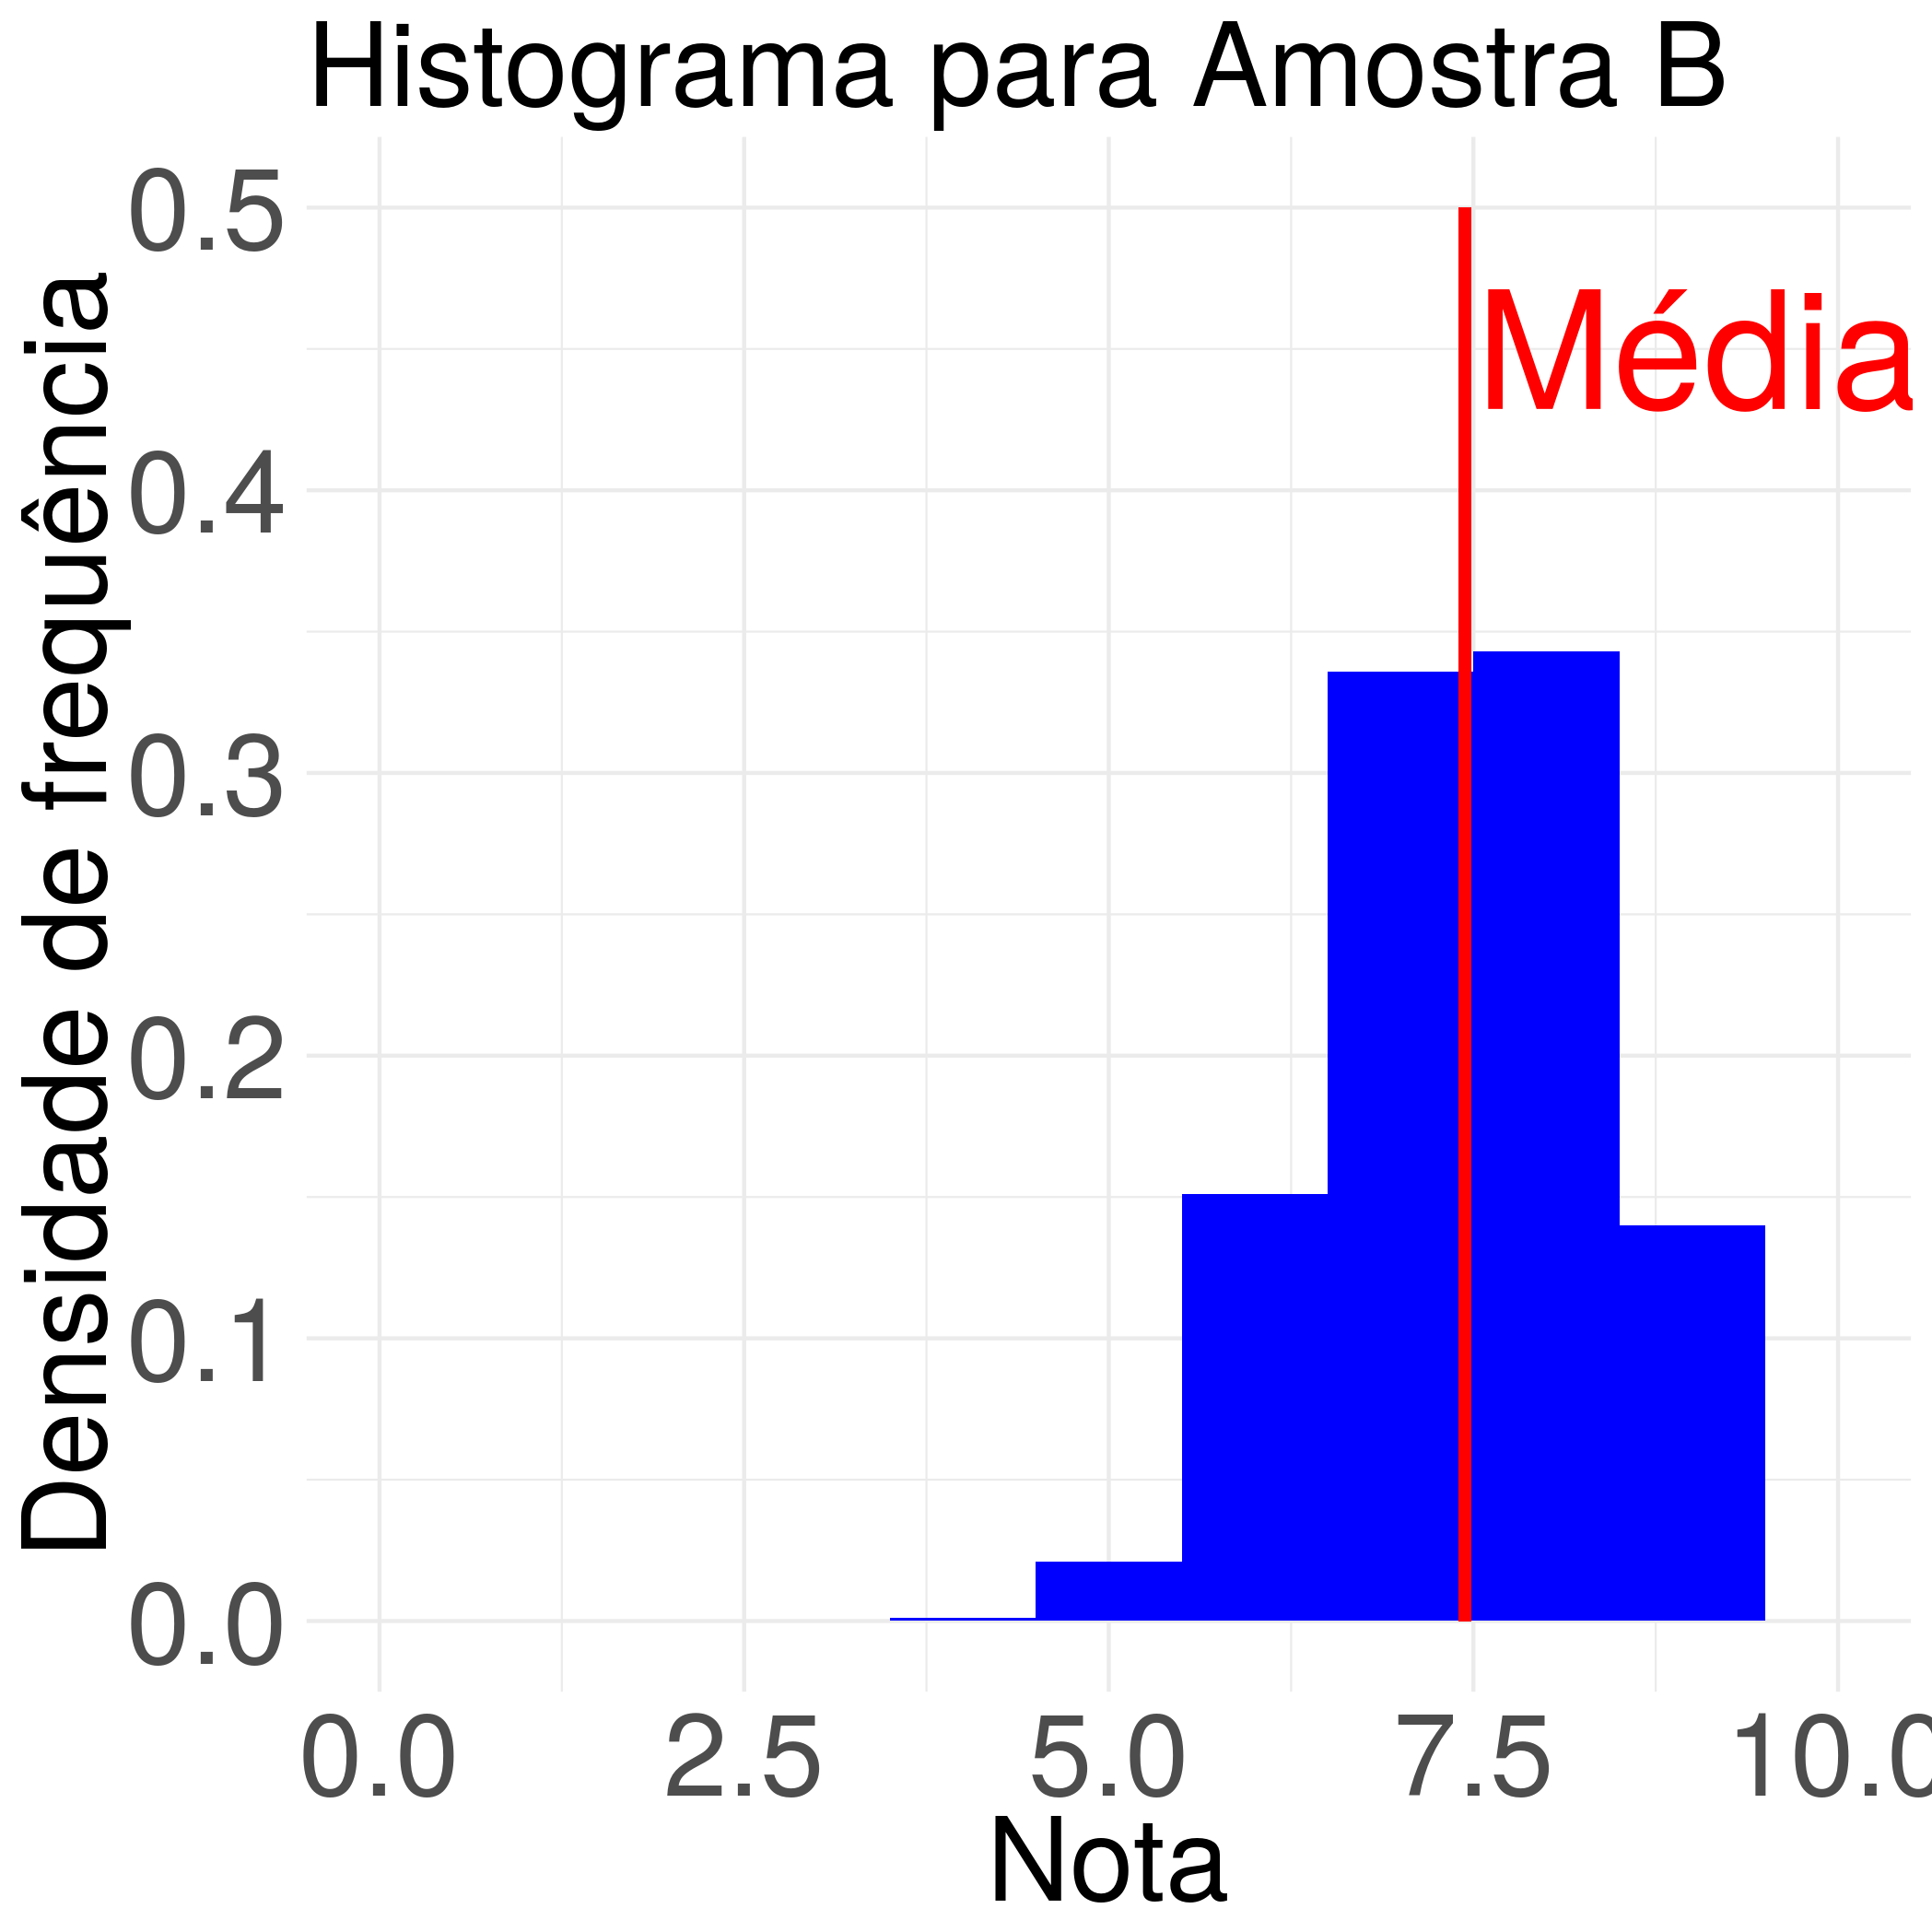
\includegraphics[width=.275\linewidth]{figures/histograma_amostra_b.png}\label{fig:amostra_b}}\\
\subfloat[Amostra C]{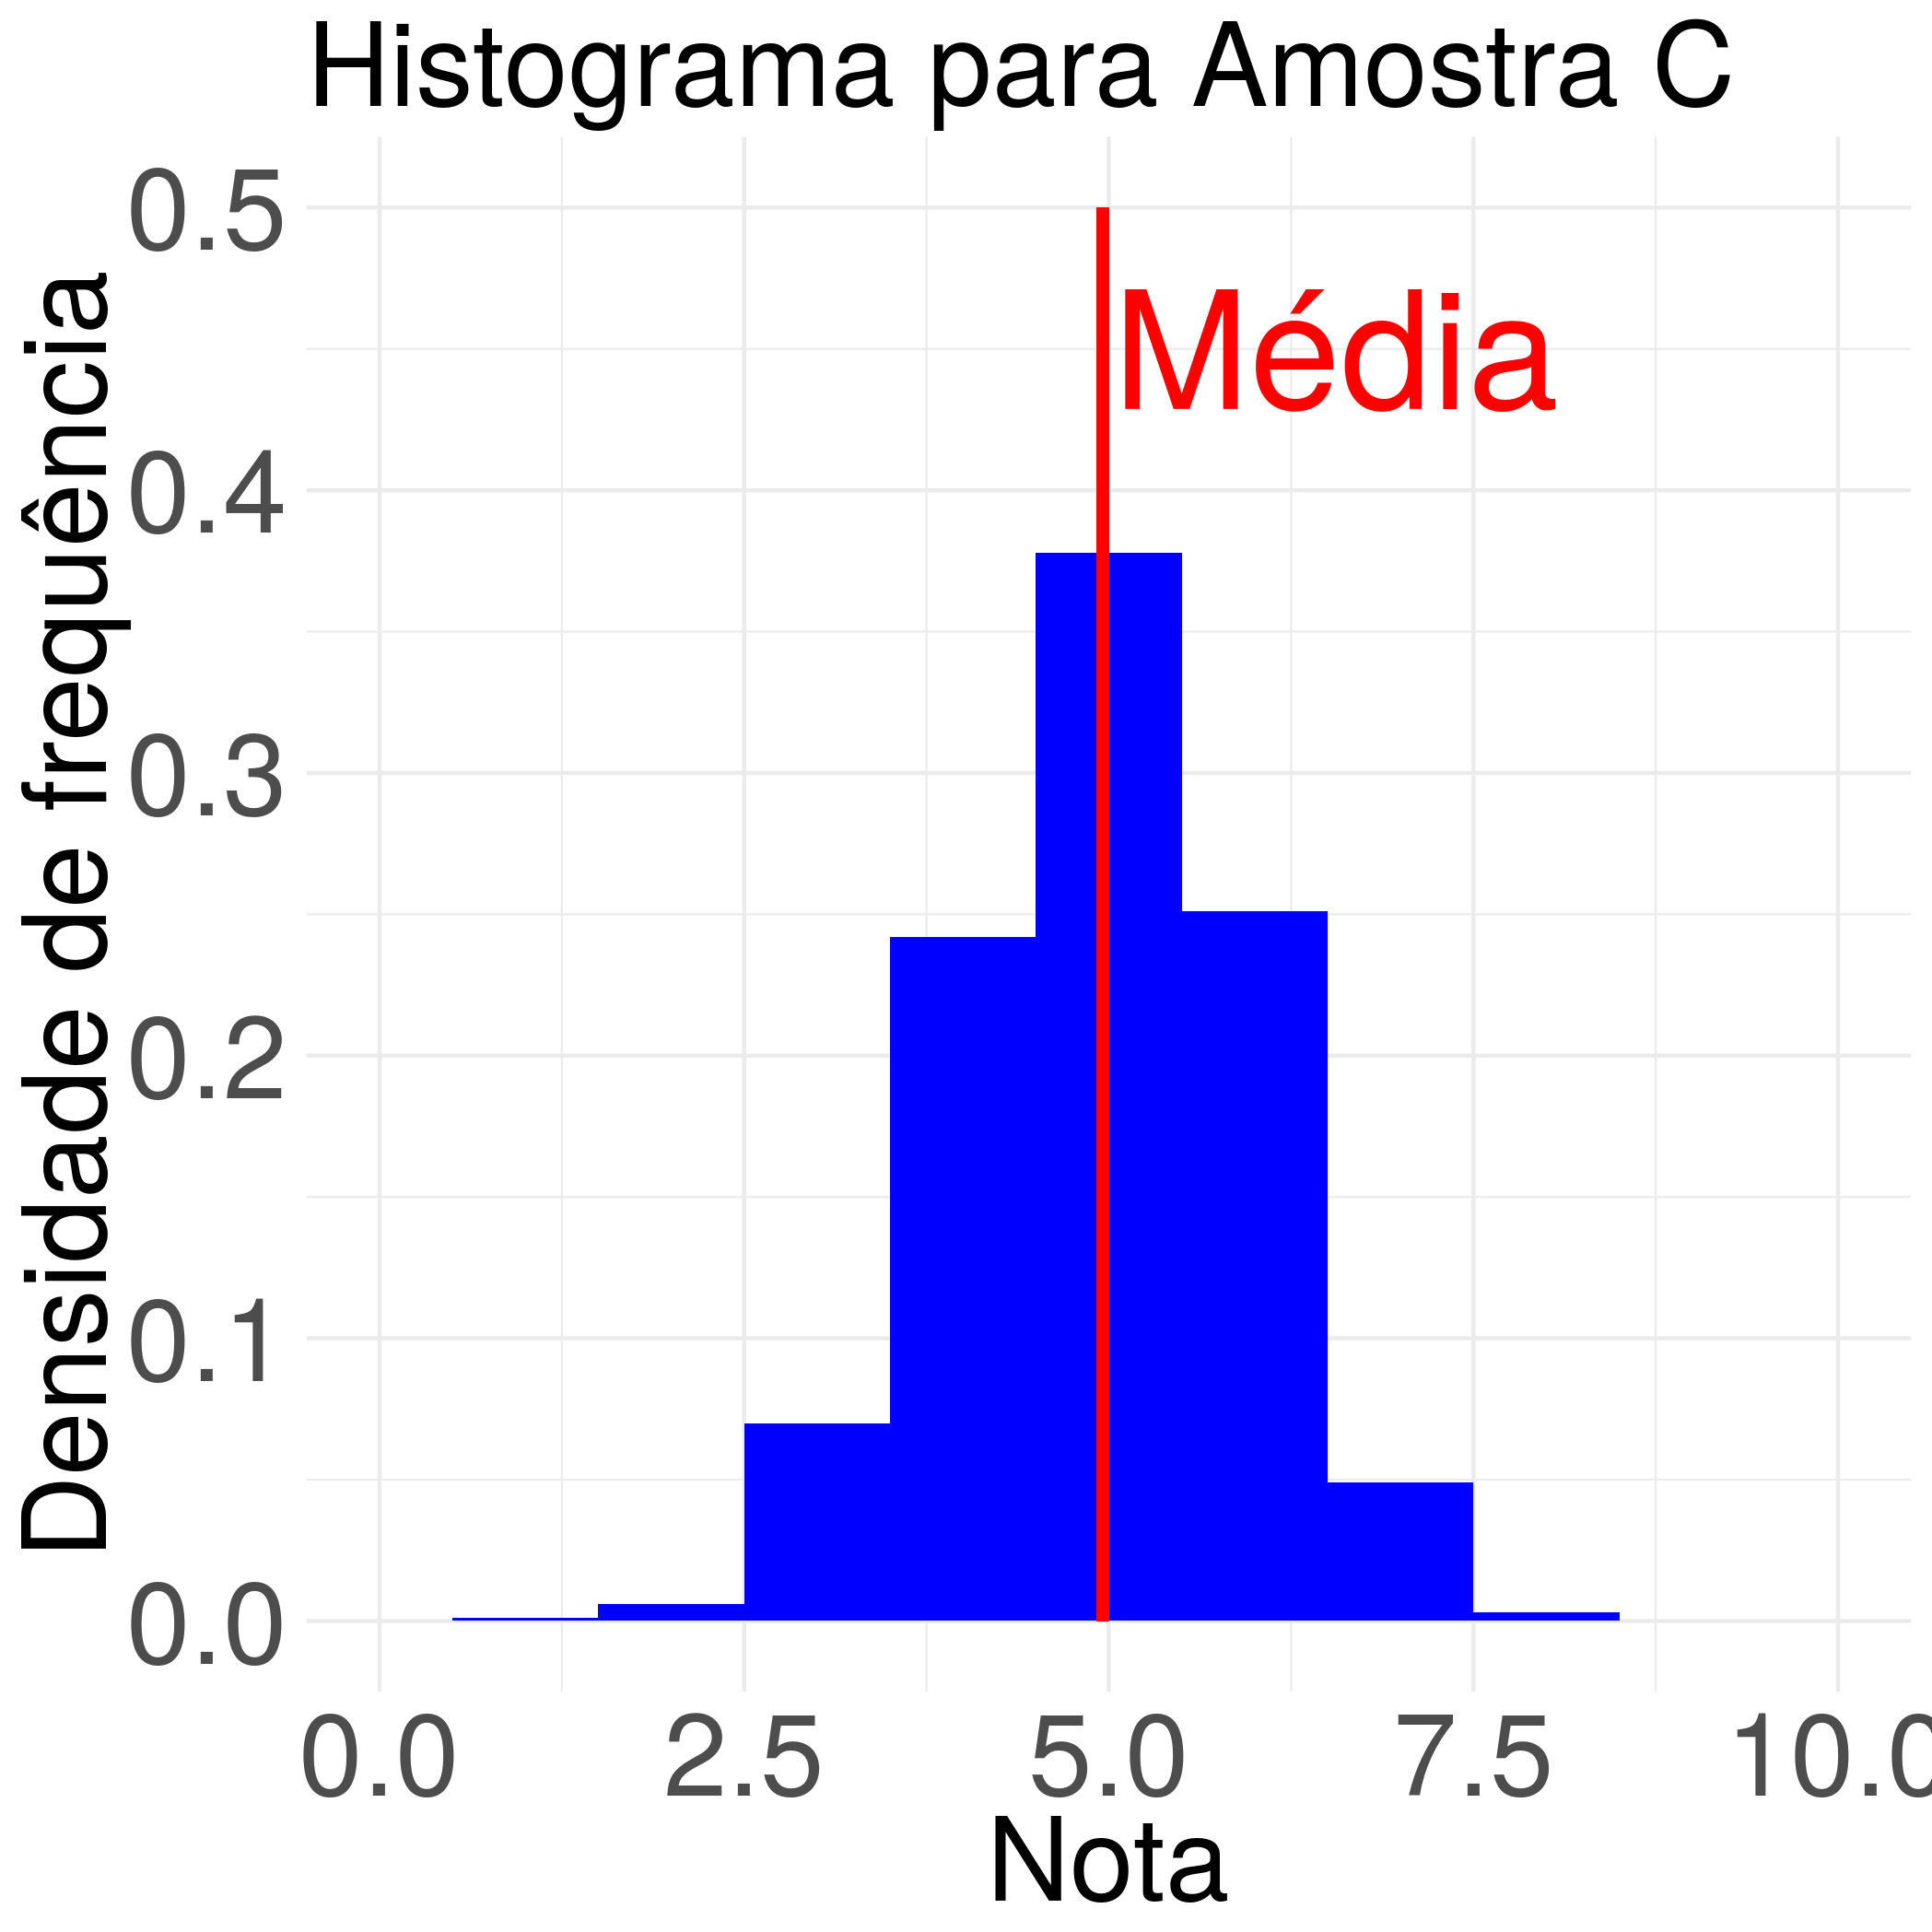
\includegraphics[width=.275\linewidth]{figures/histograma_amostra_c.png}\label{fig:amostra_c}} \hspace{0.15\linewidth}
\subfloat[População]{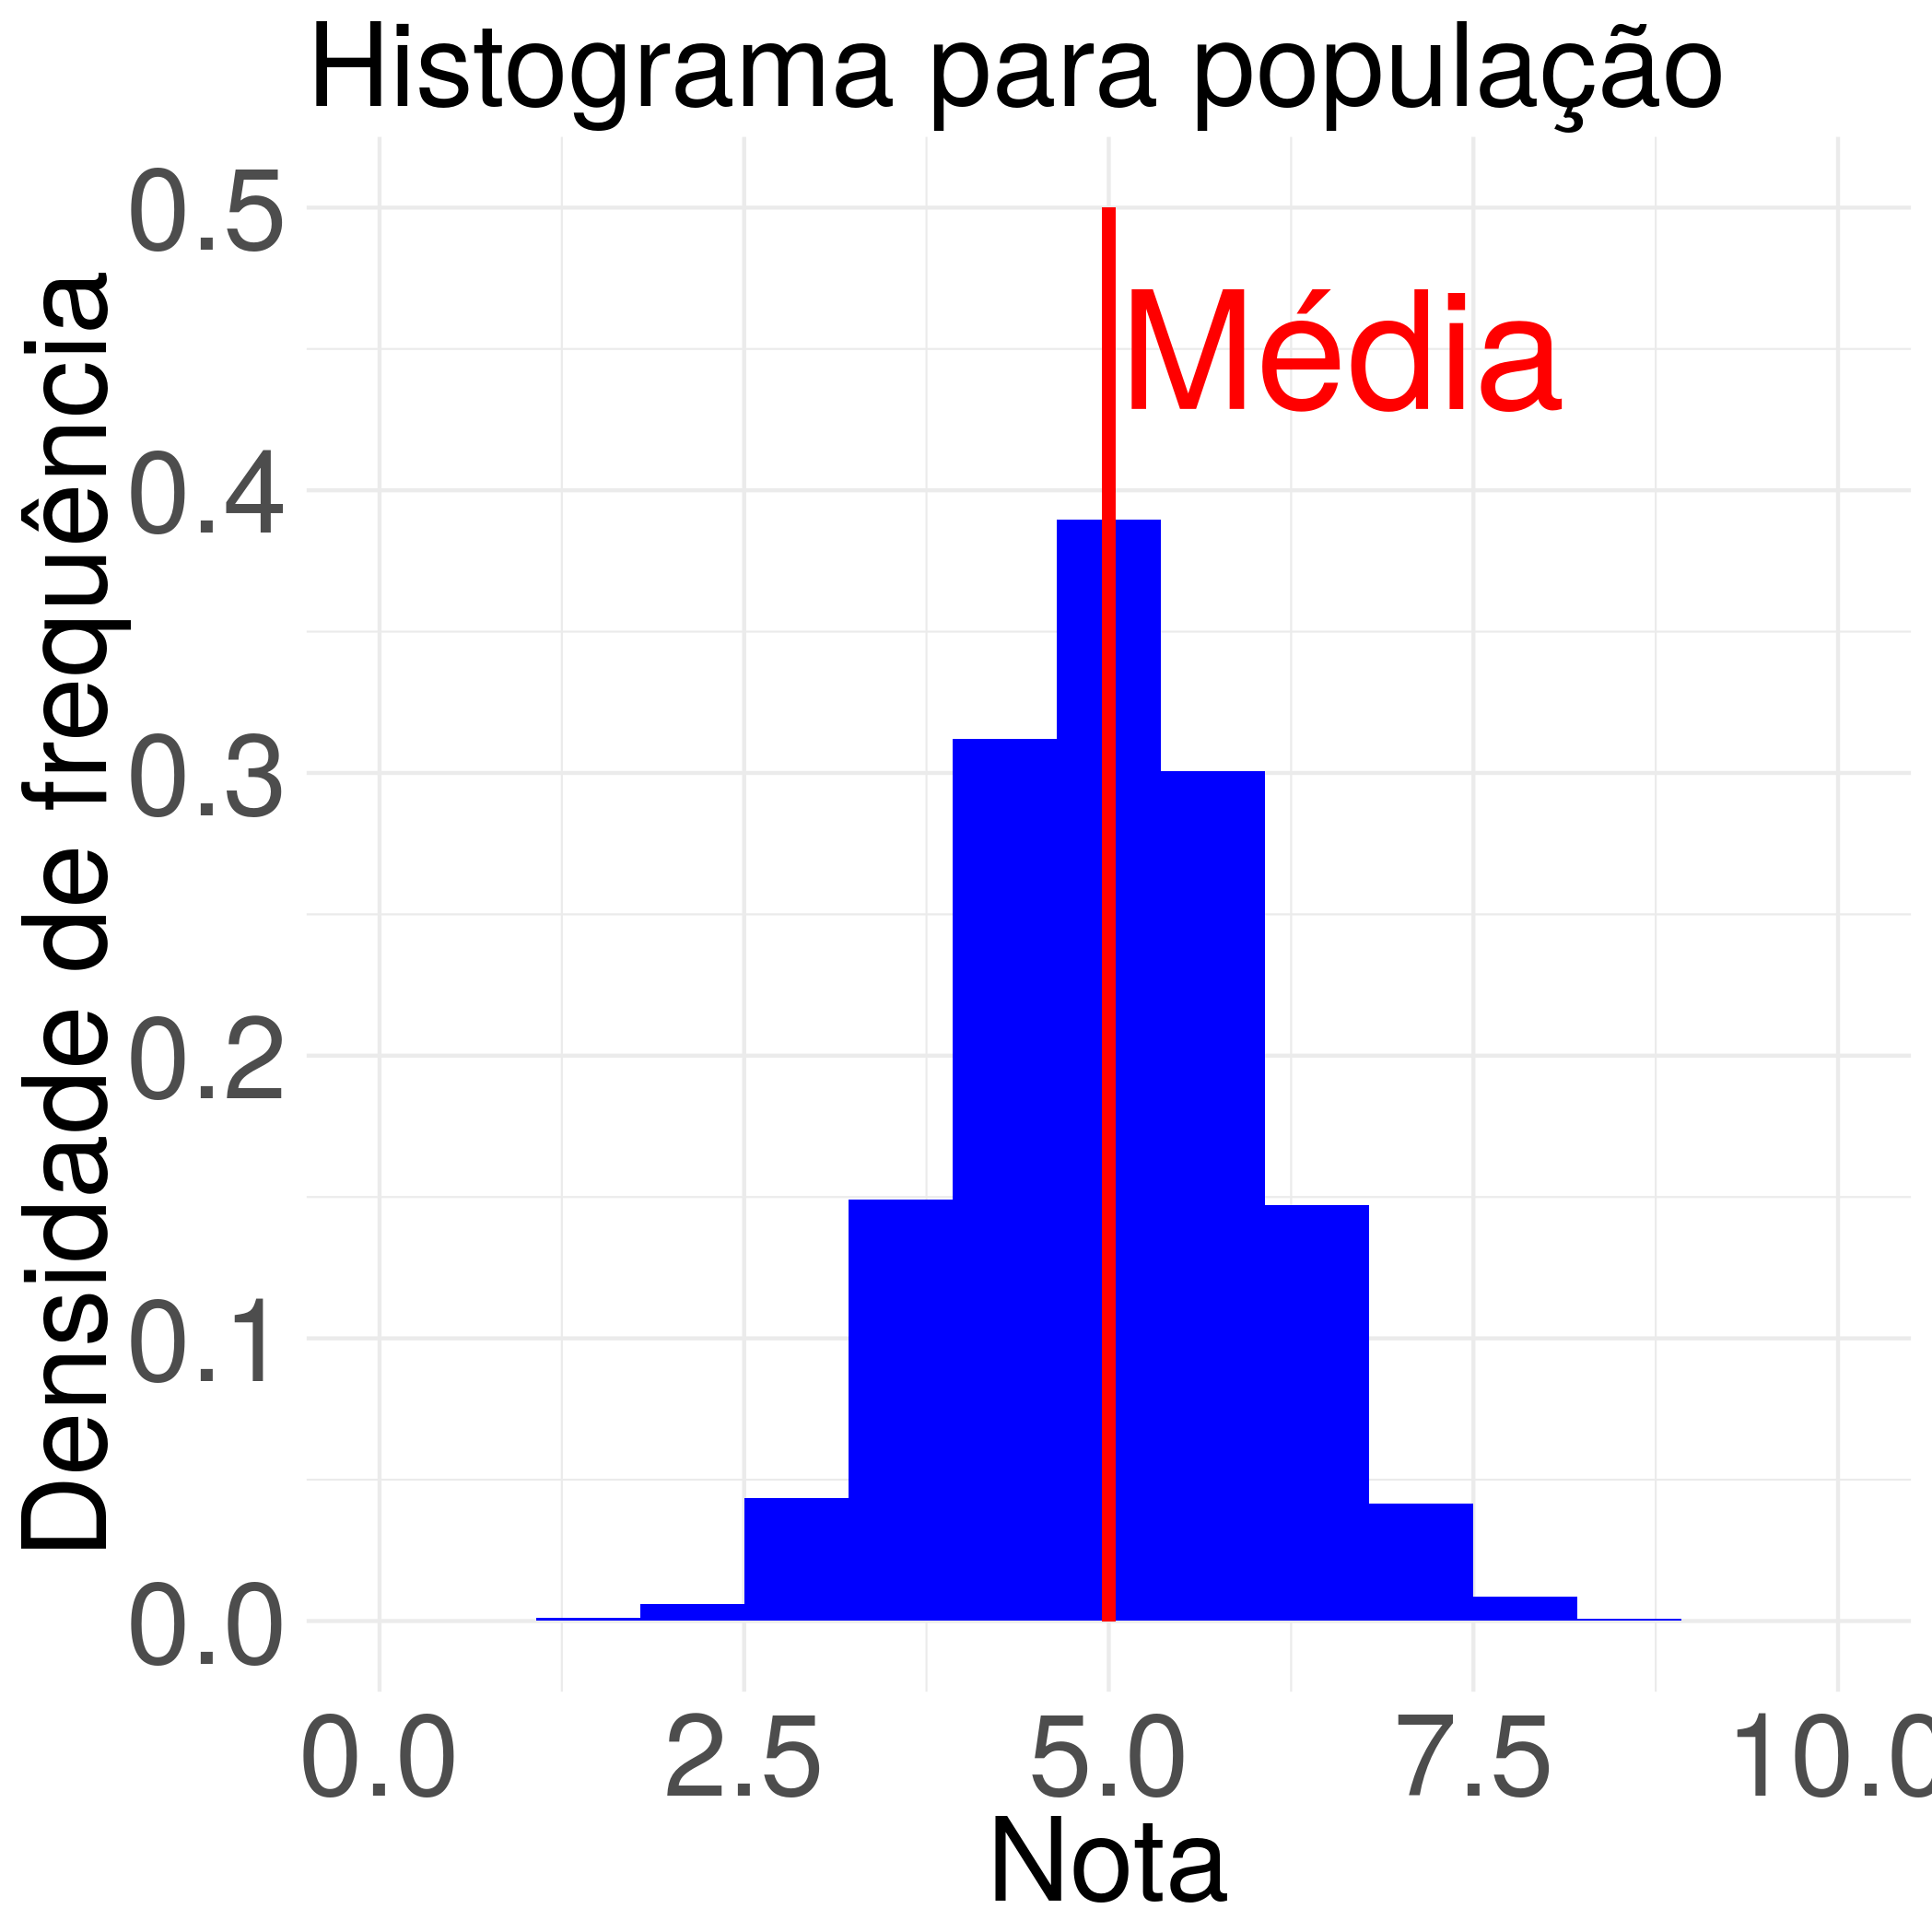
\includegraphics[width=.275\linewidth]{figures/histograma_populacao.png}\label{fig:populacao}}
\end{figure}

\end{frame}

\begin{frame}{Exemplo de motivação (Procedimento de Neyman-Pearson)}

\begin{description}
 \item[Amostra A:] A média da amostra A é menor que 5, então decidimos que a média população é menor que 5, ou seja, decidimos por $H_1$;
 \vfill
 
 \item[Amostra B:] A média da amostra B é maior que 5, então decidimos que a média da população é maior que 5, ou seja, decidimos por $H_1$;
 \vfill
 
 \item[Amostra C:] A média da amostra C é igual a 5, então decidimos que a média da população é igual a 5, ou seja, decidimos por $H_0$.
\end{description}

\begin{block}{Problema}
	Quão longe a média da amostra precisa estar de $5$ para rejeitar $H_0: \mu = 5$?
\end{block}

\begin{block}{Solução}
	Usamos estatística para determinar quão longe a média da amostra precisa estar de $5$ para rejeitar $H_0: \mu = 5$.
\end{block}
 
\end{frame}



\begin{frame}{}

\small

 A probabilidade do erro tipo I e II são denotadas por
 \begin{align*}
  \alpha &= P(\mbox{Erro tipo I}) = P(H_1 \mid H_0),\\
  \beta &= P(\mbox{Erro tipo II}) = P(H_0 \mid H_1).
 \end{align*}
\vfill
 
 {\color{blue} \textbf{Ideia}:  Tomar uma decisão que minimize simultaneamente $\alpha$ e $\beta$.} 
  \vfill
  
  {\color{red} \textbf{Problema}:  Não é possível tomar uma decisão que minimize simultaneamente $\alpha$ e $\beta$, conforme ilustrado na figua.}
  \begin{figure}[!htbp]
    \centering
    \caption{\textit{trade-off} entre $\alpha$ e $\beta$.}
      \begin{tikzpicture}[scale = 0.5]
	\draw[line width = 0.1cm, color = black] (-1,0.5) -- (5,3.5);
	\node[above, color = blue] at (-1, 0.5) {{\LARGE $\alpha$}};
	\node[above, color = blue] at (5, 3.5) {{\LARGE $\beta$}};
	\draw[fill = black] (1,0) -- (3,0) -- (2,2) ;
	\draw[fill = black] (9,0) -- (10,2) -- (11,0);
	\draw[line width = 0.1cm, color = black] (7, 3.5) -- (13,0.5);
	\node[above, color = blue] at (7, 3.5) {{\LARGE $\alpha$}};
	\node[above, color = blue] at (13, 0.5) {{\LARGE $\beta$}};
      \end{tikzpicture}
    \label{fig:alpha_beta}
   \end{figure}

  \vfill
  
  {\color{red} \textbf{Solução}:  fixar a probabilidade do erro tipo I e encontrar a decisão que minimize $\beta$.}
  \vfill
 

\textcolor{important}{\bf Notações:}
\begin{itemize}
	\item \textcolor{important}{$\alpha$: nível de significância, erro $\alpha$ ou tamanho do teste. Geralmente, usamos $\alpha=0,05$;}
	\item \textcolor{important}{$\beta$: erro $\beta$;}
	\item \textcolor{important}{$1-\beta$: poder do teste de hipóteses.}
\end{itemize}

% $\alpha$ de nível de significância e $\beta$ de poder do teste.
 
\end{frame}

\begin{frame}{Tamanho de amostra e o erro $\beta$ e erro $\alpha$.}

\normalsize
	Quando aumentamos o tamanho da amostra, o erro $\beta$ 	diminui. Abaixo usamos a seguinte regra de decisão:
	\begin{itemize}
		\item Se $4,80 \leq \bar{x} \leq 5,20$, então decidimos por $H_0$;
		\item Se $4,80 < \bar{x}$ ou $ \bar{x} > 5,20$, então decidimos por $H_1$.
	\end{itemize}
	Na tabela~\ref{tab:erros}, note que ao aumentarmos o tamanho da amostra, as probabilidades dos erros tipo I e II diminuem. 
	
	\begin{table}[htbp]
		\caption{Erro $\alpha$ e $\beta$ ao aumentarmos o tamanho da amostra.}
		\scalebox{0.70}{
		\begin{tabular}{l|ccc}
			\toprule[0.05cm]
			Tamanho da amostra & $\alpha$ & $\beta (\mu = 4,3)$ & $\beta (\mu = 5,3)$ \\ \midrule[0.05cm]
			n = 25 & 0,42371 & 0,02259 & 0,32183 \\ 
			n = 50 & 0,25790 & 0,00234 & 0,28346 \\ 
			n = 75 & 0,16586 & 0,00027 & 0,24395 \\ 
			n = 100 & 0,10960 & 0,00003 & 0,21182 \\ 
			n = 250 & 0,01141 & 0,00000 & 0,10295 \\ 
			n = 500 & 0,00035 & 0,00000 & 0,03682 \\ 
			n = 750 & 0,00001 & 0,00000 & 0,01423 \\ 
			n = 1000 & 0,00000 & 0,00000 & 0,00571 \\  \bottomrule[0.05cm]
		\end{tabular}
		}
		\label{tab:erros}
	\end{table}
\vfill

Para calcular os erros $\alpha$ e $\beta$, assumimos que a variável $X\sim N(\mu, 1,25^2)$ ($X = $ \texttt{nota}). Ou seja, $\alpha = P(\bar{X} \leq 4,80 \mid \mu = 5) + P(\bar{X} \geq 5,20 \mid \mu = 5)$ e $\beta = P\left( 4,80 \leq \bar{X} \leq 5,20 \mid \mu \right), \mu \in \left\{4,3; 5,3 \right\}$.	

\normalsize

\end{frame}

\begin{frame}{P-valor}

\normalsize

	\begin{block}{Definição}
		\begin{itemize}
			\item Vamos chamar a possibilidade ou plausibilidade ou indicação da hipótese alternativa ($H_1$) de \textit{estatística do teste};
			\item O valor-p ou nível crítico é a probabilidade de coletar uma amostra com \textit{estatística do teste} igual ou mais extrema do que a amostra observada quando $H_0$ é verdadeira. Lembre que consideramos o erro tipo I (falso positivo) tem graves consequências e as nossas decisões focam em controlar este erro;
			\item Rejeitamos $H_0$ quando o valor-p é pequeno, e usamos como valor de referência o nível de significância $\alpha$. Ilustramos essa ideia na Figura~\ref{fig:p-valor}.
		\end{itemize}			
	\begin{figure}[htbp]
		\centering
		\caption{Uso do valor-p.}
		\label{fig:p-valor}
		\begin{tikzpicture}
		\draw[->] (0,0) -- (5,0);
		\draw (1, -0.1) -- (1, 0.1);
		\draw (4, -0.1) -- (4, 0.1);
		\node [above, left] at (1, 0.3) {$H_1$};
		\node [above, right] at (4, 0.3) {$H_0$};
		\draw (2, -1) -- (2, 1);
		\node [above, right] at (2, 1) {$\alpha$};
		\draw [->] (1.9, 0.5) -- (1.2, 0.5);
		\draw [->] (2.1, 0.5) -- (2.9, 0.5);
		\node [below, left] at (6, -0.2) {valor-p};
		\node [below] at (1, -0.15) {$0$};
		\node [below] at (4, -0.15) {$1$};
		\end{tikzpicture}
	\end{figure}
	\end{block}

\normalsize

\end{frame}

\begin{frame}{P-valor como variável aleatória}

\normalsize

	\begin{block}{Exemplo}
		Imagine que temos um amostra com quatro valores de uma variável aleatória contínua com distribuição normal com desvio padrão $\sigma^2=1$ e considere as hipóteses $H_0: \mu = 0$ e $H_1: \mu \neq 0$. Usamos a seguinte ideia para decidir: Se a média da amostra $\bar{x}$ estiver longe de $\mu=0$ rejeitamos $H_0$, ou seja, rejeitamos $H_0$ se $\left\lvert \frac{(\bar{x} - 0)\sqrt{n}}{\sigma} \right\rvert $ for grande. A estatística de teste neste caso é $\left\lvert \frac{(\bar{x} - 0)\sqrt{n}}{\sigma} \right\rvert$.
		\begin{itemize}
			\item O valor-p é calculado usando $P \left( \left\lvert \frac{(\bar{X} - 0)\sqrt{n}}{\sigma} \right\rvert > \left\lvert \frac{(\bar{x} - 0)\sqrt{n}}{\sigma}  \right\rvert \mid  H_0: \mu = 0 \right)$. 
			\item Ao mudarmos a amostra, também mudamos o valor-p. Como ilustrado na Tabela~\ref{tab:p-valor}.
		\end{itemize}		

	
	\begin{table}[ht]
		\centering
		\scalebox{0.6}{
		\begin{tabular}{l|cccc|c|c|l}
			\toprule[0.05cm]
			& Valor 1 & Valor 2 & Valor 3 & Valor 4 & Estatística do teste & P-valor & Decisão \\ 
			\midrule[0.05cm]
			Amostra 1 & 0,477 & 1,965 & 0,762 & 2,997 & 3,101 & 0,002 & Rejeitamos $H_0$ \\ 
			Amostra 2 & -1,125 & 0,335 & -3,063 & -2,394 & -3,123 & 0,002 & Rejeitamos $H_0$ \\ 
			Amostra 3 & 0,412 & -1,294 & 0,220 & 0,751 & 0,045 & 0,964 & Não rejeitamos $H_0$ \\ 
			Amostra 4 & 0,448 & -1,183 & 0,299 & 0,329 & -0,054 & 0,957 & Não rejeitamos $H_0$ \\ 
			\bottomrule[0.05cm]
		\end{tabular}
		}
		\caption{Valor-p calculado para várias amostras de tamanho $n=4$ de uma variável aleatória aleatória com distribuição normal com variância $\sigma^2=1$, quando $H_0:\mu=0$ é verdadeira.} 
		\label{tab:p-valor}
	\end{table}

	\normalsize
	\end{block}


\end{frame}	

\begin{frame}{Valor-p}



Valor-p, de forma similar a média $\bar{x}$, tem um valor diferente para cada amostra, e, então, podemos interpretar o valor-p como uma observação de uma variável aleatória. Como ilustração, as Figura~\ref{fig:p-valor-h0},  Figura~\ref{fig:p-valor-h1-lower} e Figura~\ref{fig:p-valor-h1-upper} mostram histogramas para $10.000$ valores-p provenientes de $10.000$ amostras de tamanho amostral $n=4$ de uma variável aleatória contínua com distribuição normal com desvio padrão $\sigma=1$.

\begin{figure}[htbp]
	\centering
	\subfloat[][$\mu=0$]{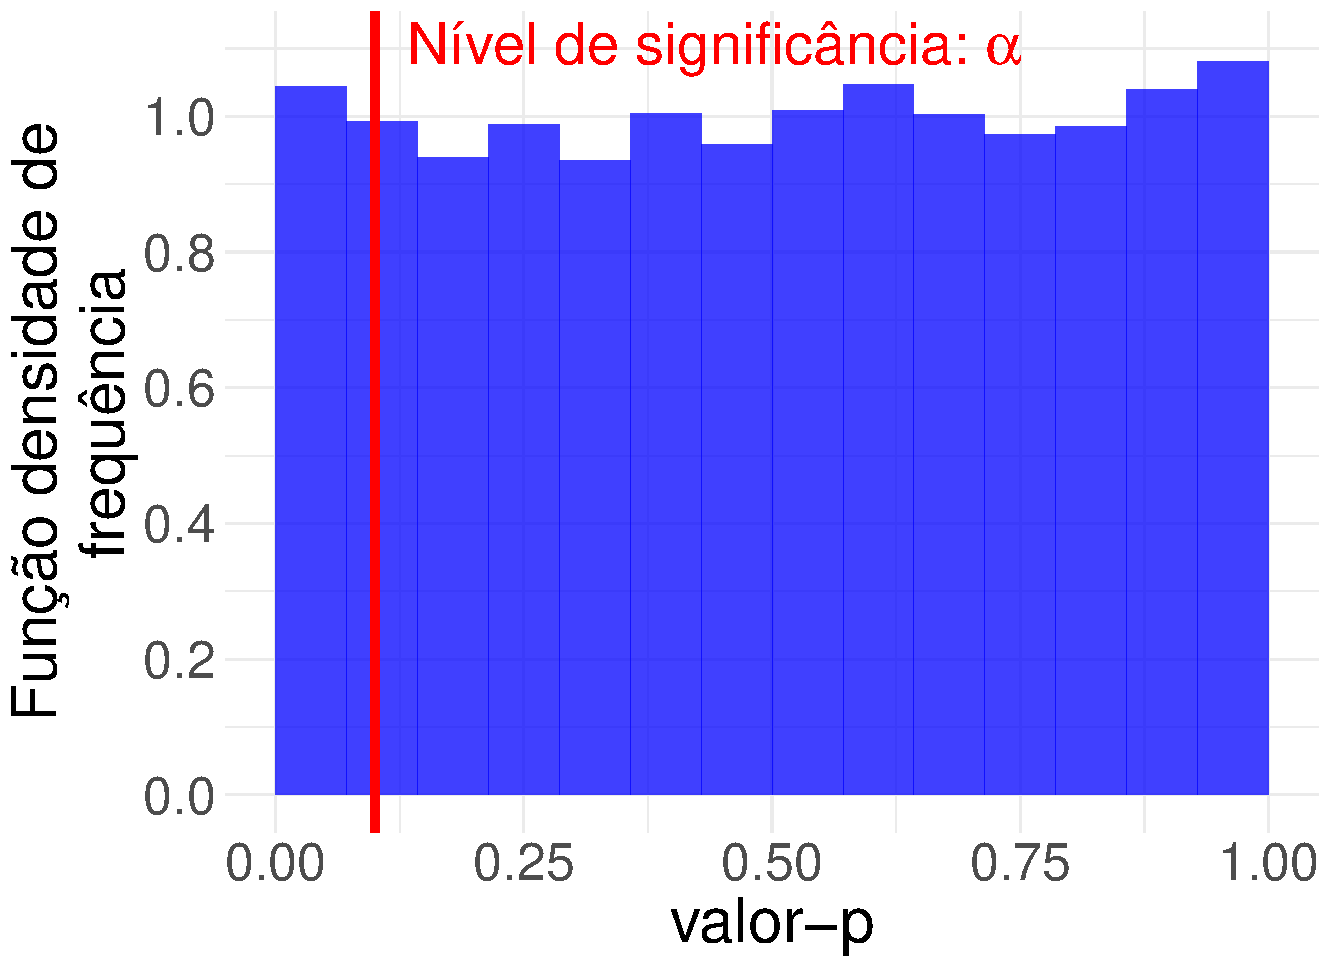
\includegraphics[width=0.33\linewidth]{figures/p_valor_h0.pdf} \label{fig:p-valor-h0}}
	\subfloat[][$\mu=-1$]{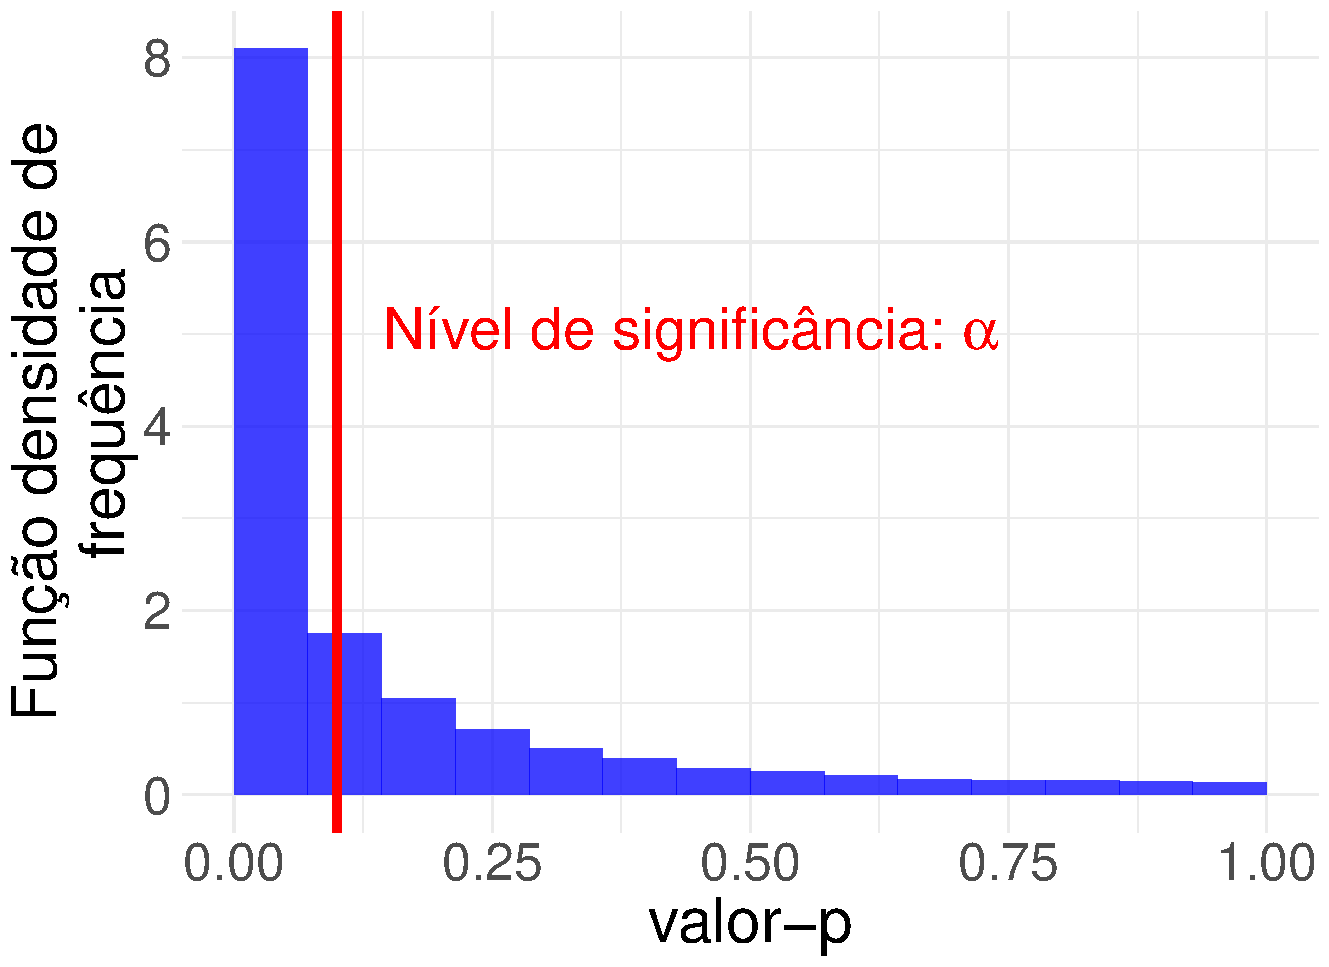
\includegraphics[width=0.33\linewidth]{figures/p_valor_h1_lower.pdf} \label{fig:p-valor-h1-lower}}
	\subfloat[][$\mu=1$]{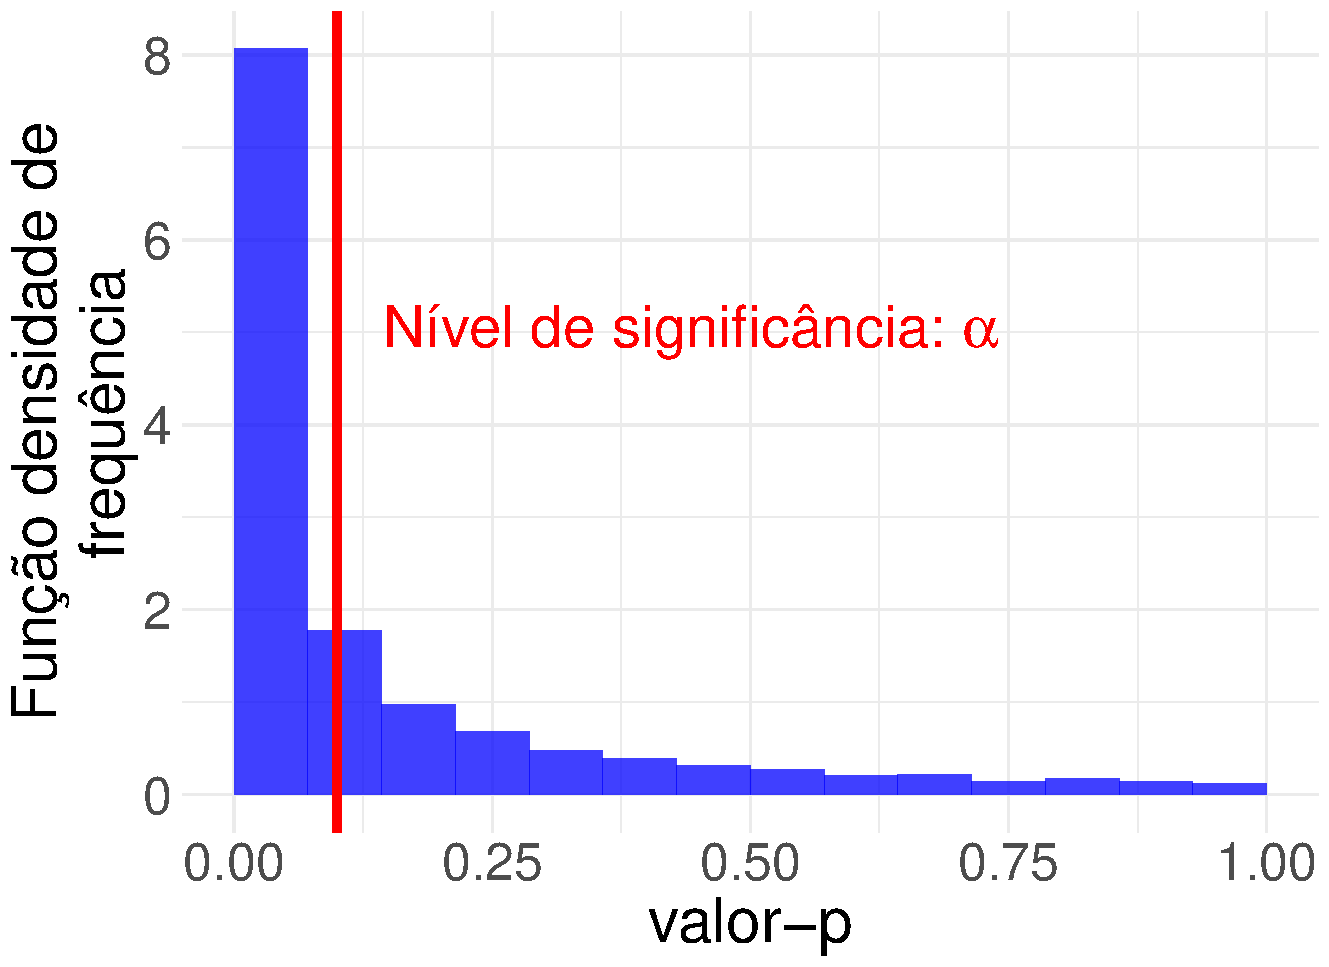
\includegraphics[width=0.33\linewidth]{figures/p_valor_h1_upper.pdf} \label{fig:p-valor-h1-upper}}
	\caption{ Histograma de valores-p para $10.000$ amostras quando (a) $H_0: \mu=0$ é verdadeira, (b) $H_1: \mu \neq 0$ é verdadeira e $\mu=-1$, e (c)  $H_1: \mu \neq 0$ é verdadeira e $\mu=1$.}
\end{figure}
\normalsize


\end{frame}

%\begin{frame}{title}
%
%\begin{figure}[htbp]
%	\centering
%	\subfloat[][$\mu=0$]{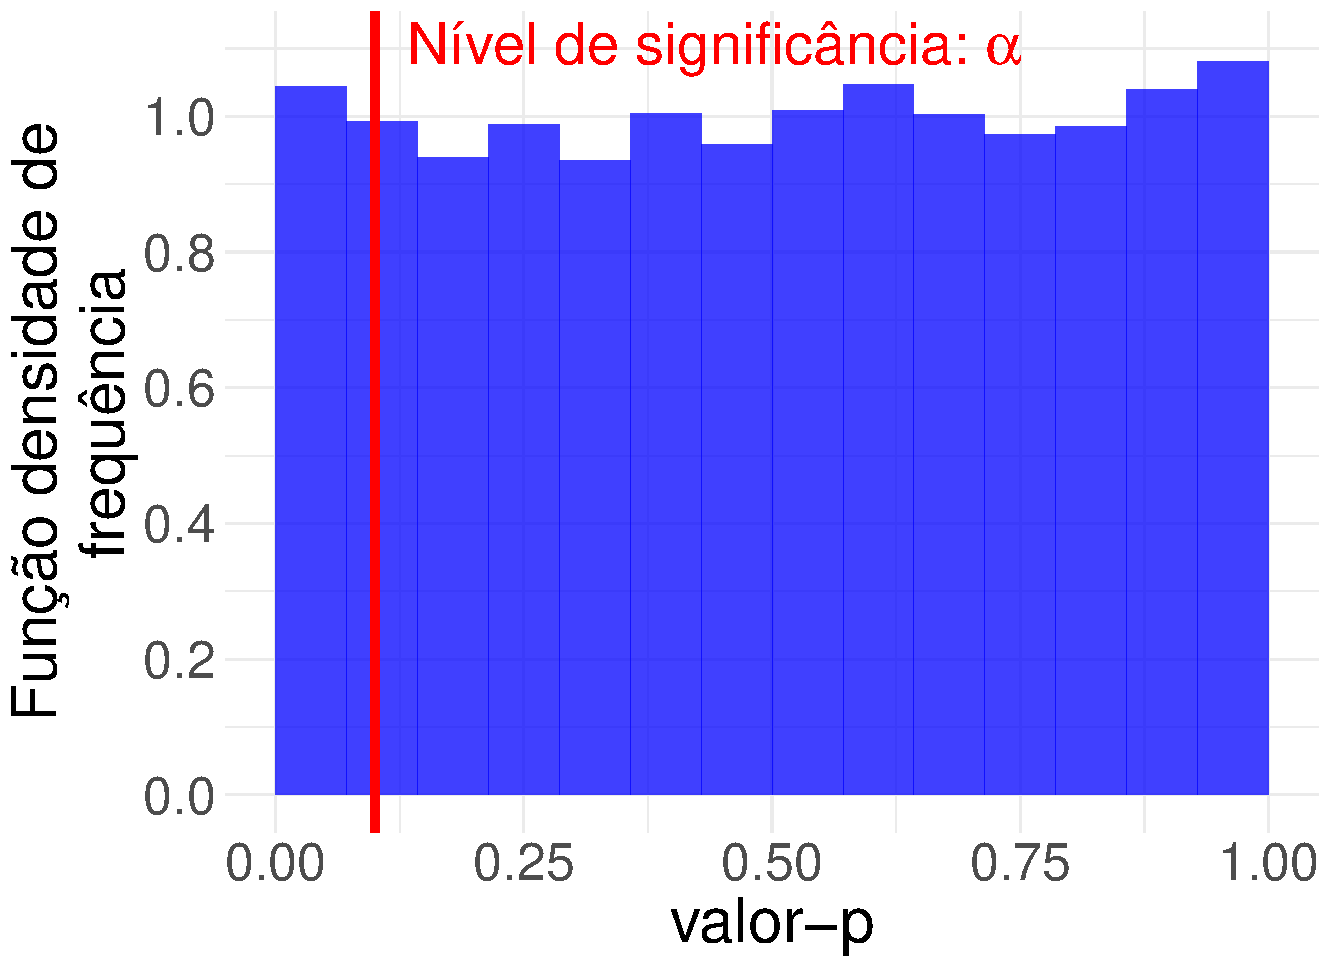
\includegraphics[width=0.33\linewidth]{figures/p_valor_h0.pdf} \label{fig:teste1}}
%	\subfloat[][$\mu=-1$]{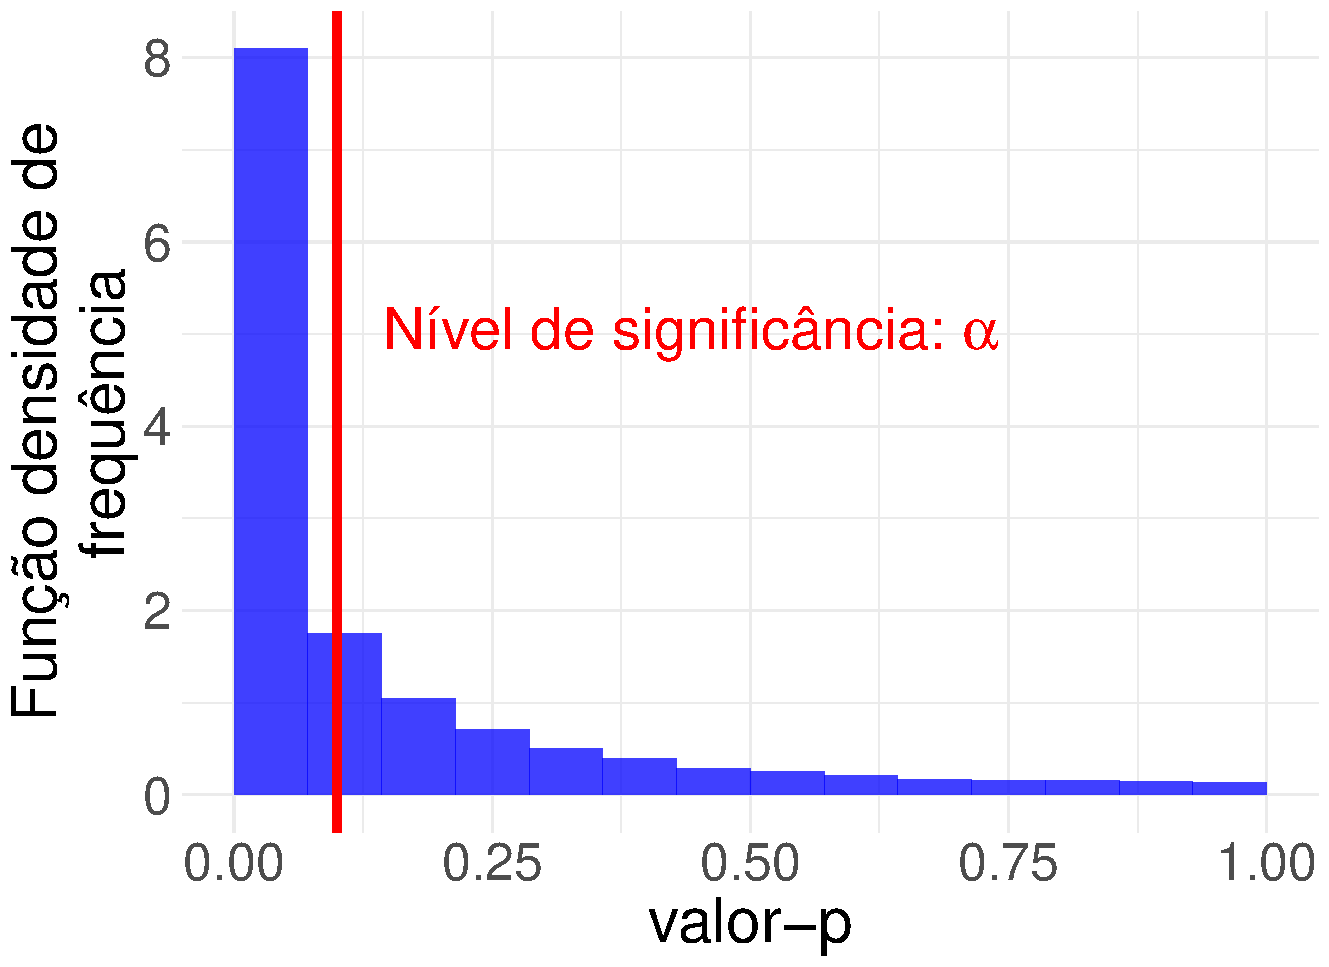
\includegraphics[width=0.33\linewidth]{figures/p_valor_h1_lower.pdf} \label{fig:teste2}}
%	\subfloat[][$\mu=1$]{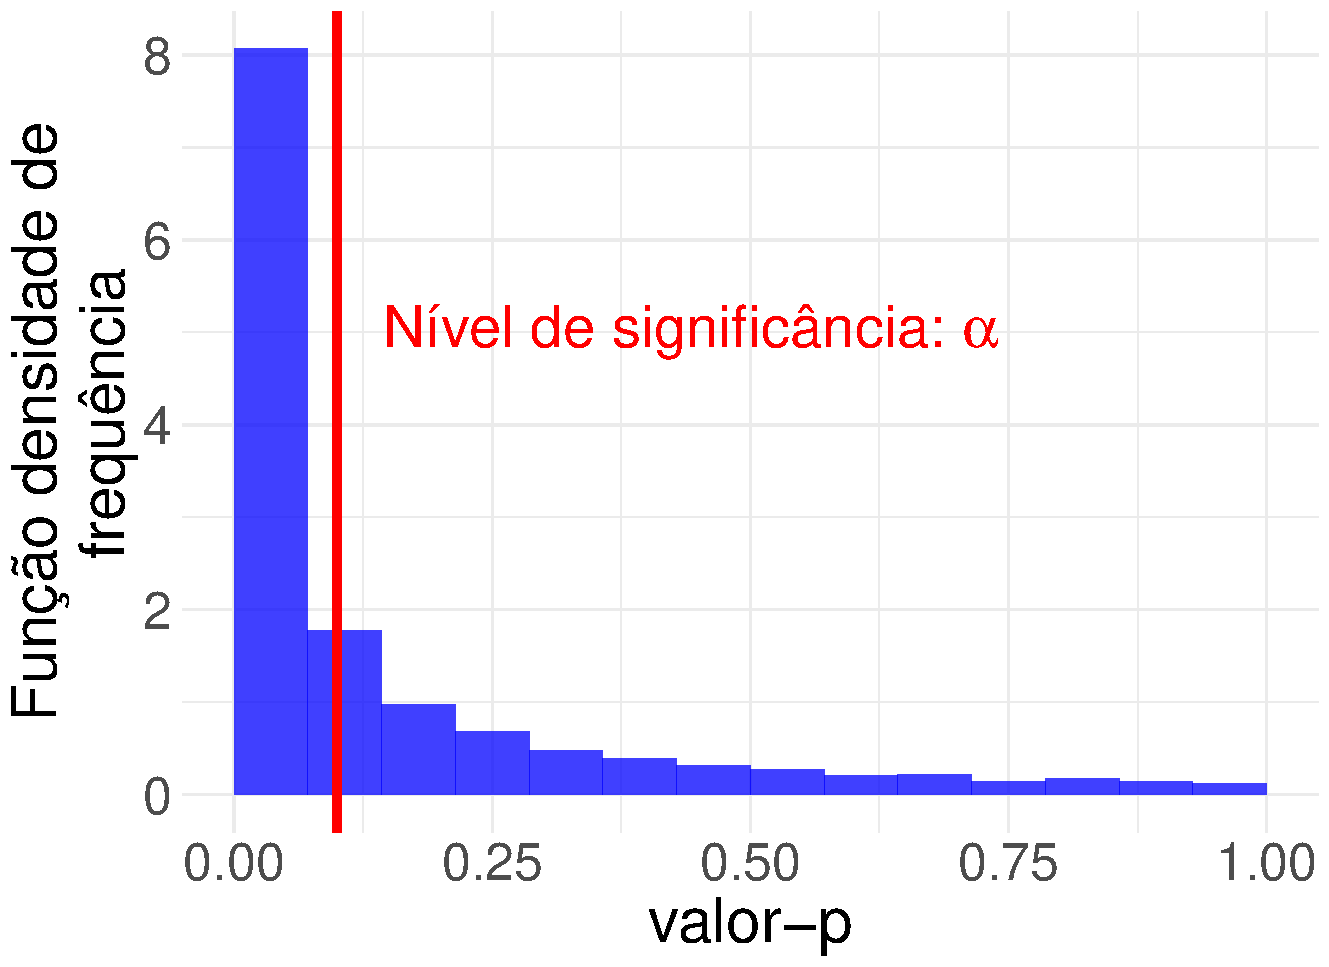
\includegraphics[width=0.33\linewidth]{figures/p_valor_h1_upper.pdf} \label{fig:teste3}}
%	\caption{ Histograma de valores-p para $10.000$ amostras quando (a) $H_0: \mu=0$ é verdadeira, (b) $H_1: \mu \neq 0$ é verdadeira e $\mu=-1$, e (c)  $H_1: \mu \neq 0$ é verdadeira e $\mu=1$.}
%\end{figure}
%
%Teste 1~\ref{fig:teste1}, teste 2~\ref{fig:teste2} e teste 3~\ref{fig:teste3}.
%
%\end{frame}

\section{Teste de hipóteses deste curso}

\begin{frame}{Testes de hipóteses}


Nesse curso, vamos determinar a regra de decisão, chamada de ``Teste de Hipóteses'' para os seguintes problemas:

\begin{enumerate}

	\item Uma variável ou população:
		\begin{enumerate}[a.]
			\item Teste  para média $\mu$, para distribuição normal com $\sigma^2$ conhecido (teste $Z$);
			\item Teste para média $\mu$, para distribuição com $\sigma^2$ desconhecido (teste $t$);
			\item Teste para $\sigma^2$ (teste qui-quadrado para variância);
			\item Teste para proporção $p$,  para distribuição Bernoulli quando $n \geq 40$.
		\end{enumerate}
	\vfill
	
	\item Duas variáveis ou duas populações:
	\begin{enumerate}[a.]
			\item Teste para diferença de médias $\mu_1 - \mu_2$, para distribuição normal com $\sigma^2$ conhecido;
		
		\item Teste para razão de variâncias $\frac{\sigma_1^2}{\sigma_2^2}$, para distribuição normal (teste F);
		
		\item Teste para diferenças de médias $\mu_1 - \mu_2$, para distribuição normal com $\sigma^2$ desconhecido;
		\begin{enumerate}[i.]
			\item Variâncias das duas populações ou variáveis são iguais;
			\item Variâncias das duas populações ou variáveis são diferentes;
		\end{enumerate}
		
		\item Teste $t$ pareado;
		
		\item Teste para diferença de proporções $p_1 - p_2$, para distribuição Bernoulli quando $n \geq 40$;
		
		\item Teste de associação entre duas variáveis qualitativas;
		
		\item Teste de associação entre duas variáveis quantitativas.
		
	\end{enumerate}
\end{enumerate}

 
\end{frame}

\subsection{Passos para testar $H_0$ e $H_1$.}

\begin{frame}{Etapas para construir um teste.}

\normalsize

\begin{block}{Procedimento de Neyman-Pearson}
 Usando o procedimento de Neymann-Pearson:
 \begin{enumerate}[1)]
  \item Estabelecer as hipóteses $H_0$ e $H_1$;
  \vfill
  
  \item Estabelecer o nível de significância $\alpha$;
  \vfill
  
  \item Identificar a ``ideia'' da decisão (estatística do teste);
  \vfill
  
  \item Encontrar o(s) valor(es) crítico(s);
  \vfill
  
  \item Tomar a decisão.
 \end{enumerate}
\end{block}

\begin{block}{valor-p}
 
 Usando o valor-p
 \begin{enumerate}[1)]
    \item Estabelecer as hipóteses $H_0$ e $H_1$;
  \vfill
  
  \item Estabelecer o nível de significância $\alpha$;
  \vfill
  
  \item Encontrar o valor-p;
  \vfill
  
  \item Decidir usando o valor-p e o nível de significância.
 \end{enumerate}
\end{block}

Observação:
\begin{itemize}
	\item Alguns livros chamam o ``Procedimento de Neyman-Pearson'' de ``Procedimento Geral de Testes de hipóteses.''
\end{itemize}



\normalsize
\end{frame}

\section{Teste para $\mu$ quando $N(\mu, \sigma^2)$ com $\sigma^2$ conhecida (Teste Z).}

\begin{frame}{Distribuição normal com $\sigma^2$ conhecido (Teste Z).}

\large

Sejam
\begin{itemize}
	\item $x_1, \dots, x_n$ valores amostrados de $N(\mu, \sigma^2)$;
	\item $\sigma^2$ conhecido;
	\item $\alpha$ é o nível de significância (estabelecido pelo pesquisador e geralmente $\alpha=5\%$). 
\end{itemize}
\vfill

Queremos testar as seguintes hipóteses:
\begin{itemize}
	\item Teste bilateral: $H_0: \mu= \mu_0$ e $H_1: \mu \neq \mu_0$;
	\item Teste unilateral: $H_0: \mu \leq \mu_0$ e $H_1: \mu > \mu_0$;
	\item Teste unilateral: $H_0: \mu \geq \mu_0$ e $H_1: \mu < \mu_0$.
\end{itemize}
\vfill

\textbf{Ideia:} Primeiro calculamos a distância padronizada de $\bar{x}$ e $\mu_0$: $Z_0 = \frac{(\bar{x} - \mu_0) \sqrt{n}}{\sigma}$. Então, 
\begin{itemize}
	\item Teste bilateral: Rejeitamos $H_0: \mu - \mu_0 =0$ se $\lvert Z_0 \rvert$ for grande;
	\item Teste unilateral: Rejeitamos $H_0: \mu - \mu_0 \leq 0$ se $Z_0 $ for grande;
	\item Teste unilateral: Rejeitamos $H_0: \mu - \mu_0 \geq 0$ se $Z_0 $ for pequeno.
\end{itemize}


\normalsize
\end{frame}

\begin{frame}{Distribuição normal com $\sigma^2$ conhecido (Teste t).}


\begin{figure}[htbp]
	\centering
	\subfloat[][Teste bilateral.]{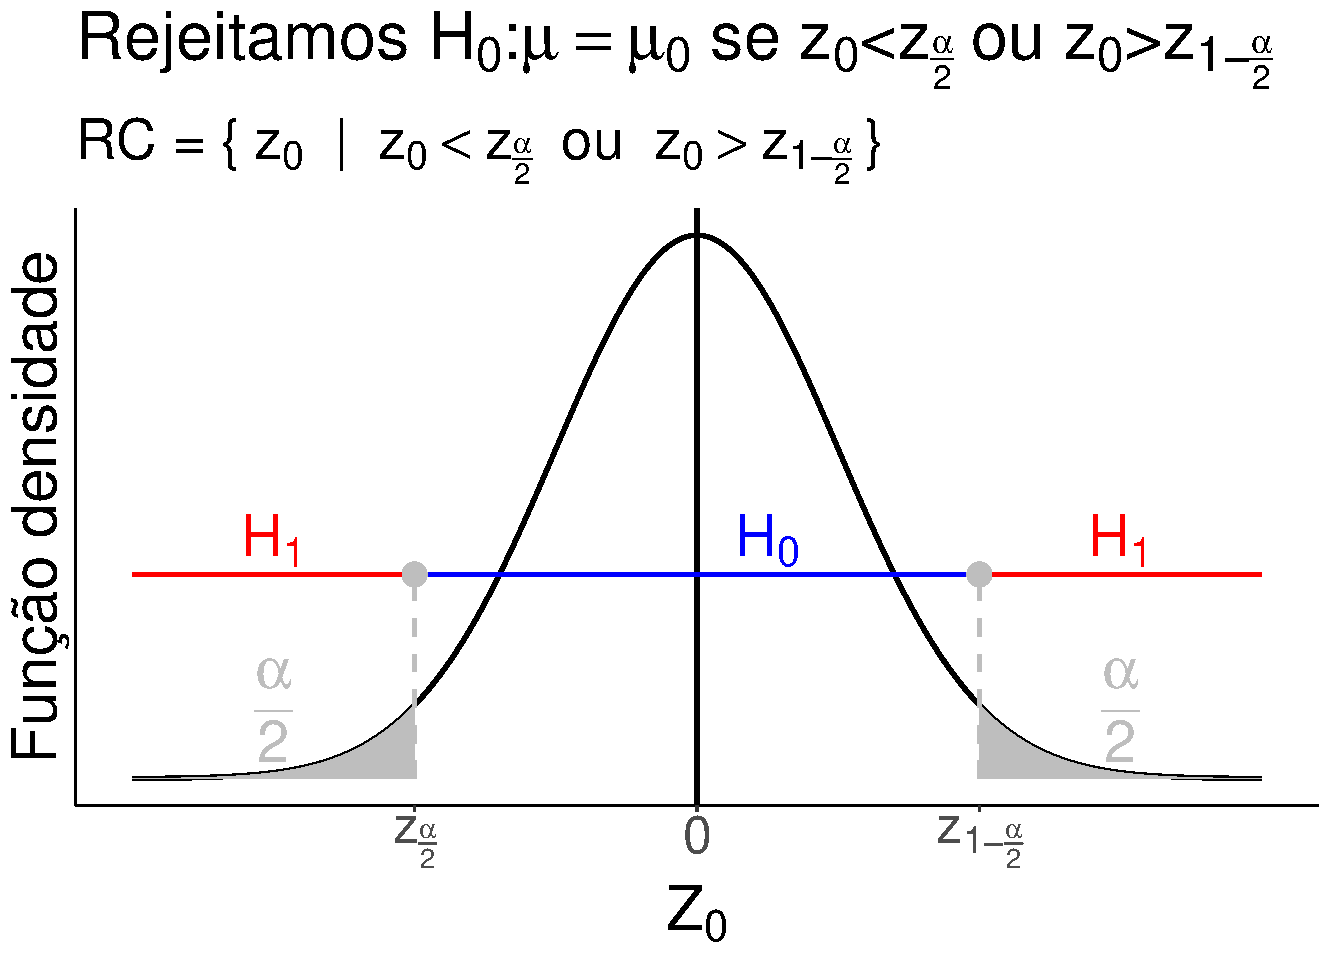
\includegraphics[width=0.32\linewidth]{figures/bilateral.pdf} \label{fig:normal-s2-bilateral}} \hfill
	\subfloat[][Teste unilateral.]{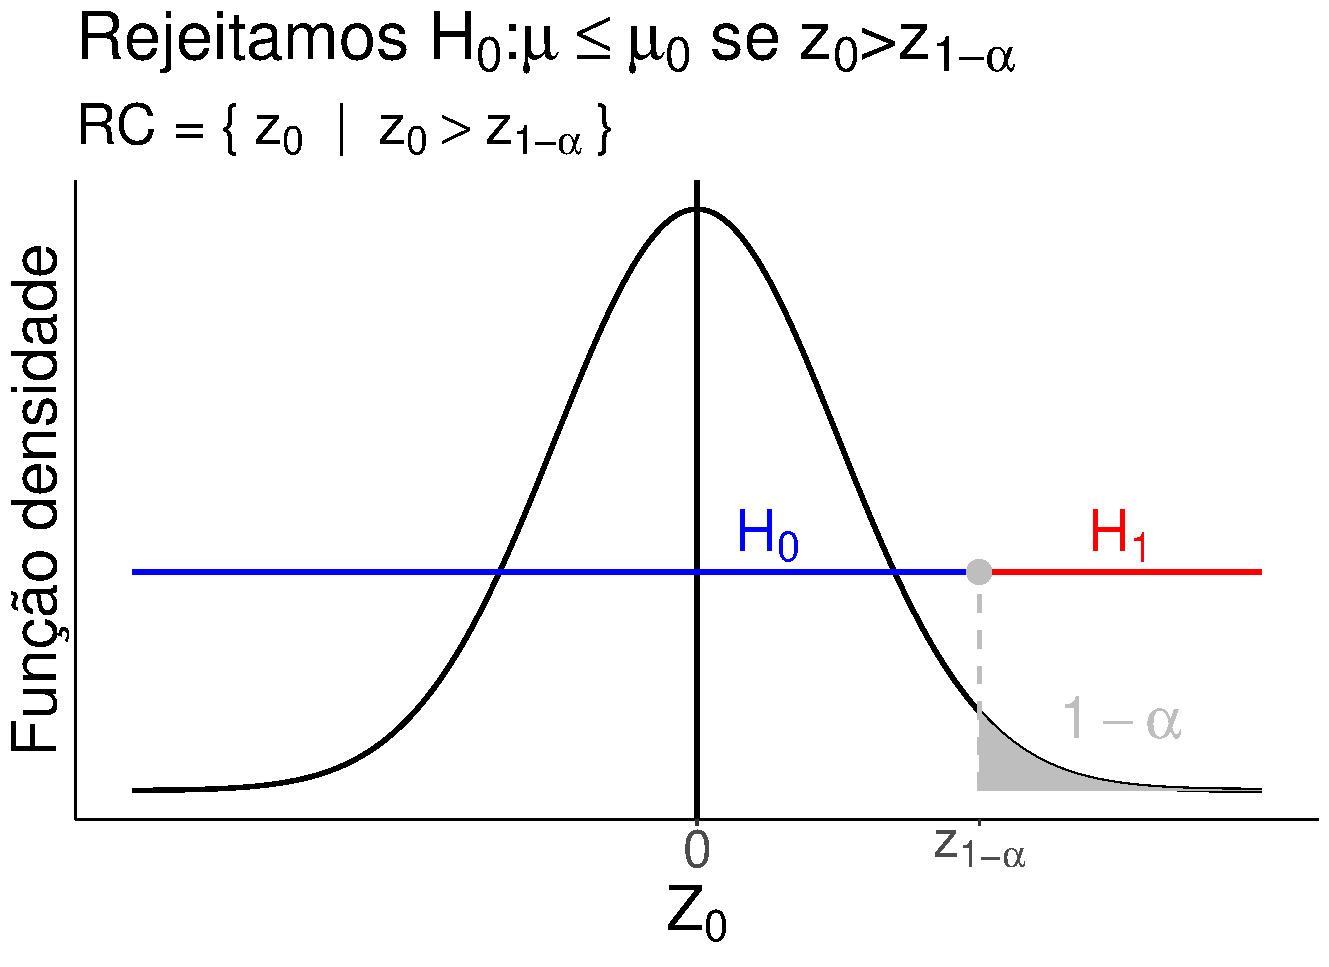
\includegraphics[width=0.32\linewidth]{figures/unilateral-h0-lower.pdf} \label{fig:normal-s2-uni-lower}} \hfill
	\subfloat[][Teste unilateral.]{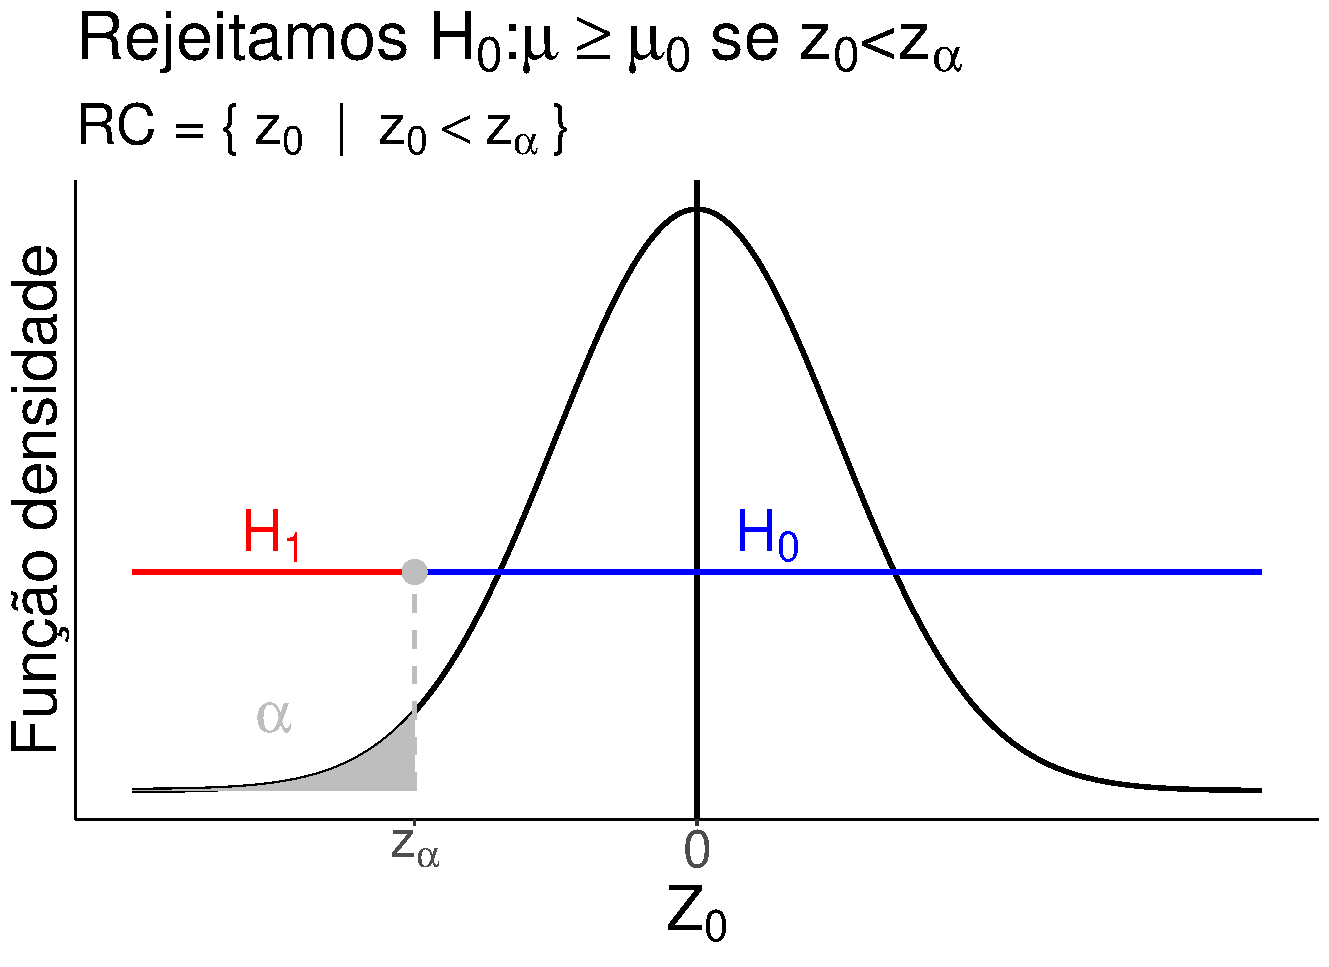
\includegraphics[width=0.32\linewidth]{figures/unilateral-h0-upper.pdf} \label{fig:normal-s2-uni-upper}}
	\caption{Região crítica para o teste Z.}
\end{figure}

\end{frame}

\begin{frame}{Distribuição normal com $\sigma^2$ conhecido (Teste t).}

\large

\begin{itemize}
	\item Na Figura~\ref{fig:normal-s2-bilateral}, testamos $H_0: \mu = \mu_0$ versus $H_1: \mu \neq \mu_0$. Rejeitamos $H_0$ se $z_0 = \frac{(\bar{x} - \mu_0)\sqrt{n}}{\sigma} \in \allowbreak RC=\{z_0 \mid z_0 < z_\frac{\alpha}{2} \mbox{ ou } z_0 > z_{1-\frac{\alpha}{2}} \}$, em que $\Phi\left( z_\frac{\alpha}{2} \right) = \frac{\alpha}{2}$ e $\Phi\left( z_{1-\frac{\alpha}{2}} \right) = 1- \frac{\alpha}{2}$;
	\vfill
	
	\item Na Figura~\ref{fig:normal-s2-uni-lower}, testamos $H_0: \mu \leq \mu_0$ versus $H_1: \mu > \mu_0$. Rejeitamos $H_0$ se $z_0 = \frac{(\bar{x} - \mu_0)\sqrt{n}}{\sigma} \in \allowbreak RC=\{z_0 \mid z_0 > z_{1-\alpha}  \}$, em que $\Phi\left( z_{1-\alpha} \right) =1- \alpha$;
	\vfill
	
	\item Na Figura~\ref{fig:normal-s2-uni-upper}, testamos $H_0: \mu \geq \mu_0$ versus $H_1: \mu < \mu_0$. Rejeitamos $H_0$ se $z_0 = \frac{(\bar{x} - \mu_0)\sqrt{n}}{\sigma} \in \allowbreak RC=\{z_0 \mid z_0 < z_{\alpha}  \}$, em que $\Phi\left( z_{\alpha} \right) = \alpha$.
\end{itemize}
Chamamos $z_\alpha$, $z_{1-\alpha}$, $z_\frac{\alpha}{2}$ e $z_{1-\frac{\alpha}{2}}$ são chamados de valores críticos.
\normalsize

\end{frame}


\begin{frame}{Distribuição normal com $\sigma^2$ conhecido (Teste Z).}

\large

\begin{block}{Exemplo}
Um pesquisador deseja estudar o efeito de certa substância no tempo de reação de seres vivos a um certo tipo de estímulo. 
Um experimento é desenvolvido com cobaias que são inoculadas com a substância e submetidas a um estímulo elétrico, com seu tempo de reação (em segundos) anotados. 
Os seguintes valores foram obtidos: 9,1; 7,2; 13,3; 10,9; 7,2; 9,9; 8,0; 8,6; 8,0; 7,1. Admite-se que o tempo de reação tem desvio padrão de 2 segundos. Além disso, da literatura médica, o pesquisador sabe que o tempo de reação ao estímulo é, em média, 8 segundos.
O pesquisador desconfia que o tempo médio sofre alteração por influência da substância. Usando um nível de significância $5\%$, o pesquisador está correto? 
\end{block}

\normalsize

\end{frame}

\begin{frame}{Distribuição normal com $\sigma^2$ conhecido (Teste Z).}

\begin{block}{Solução}

\textbf{Passo 1)} Temos duas hipóteses: $H_0:  \mu = \mu_0$ e $H_1:  \mu \neq \mu_0,$, em que $\mu_0=8$.

\textbf{Passo 2)} $\alpha = 0,05$.

\textbf{Passo 3)} Rejeitamos $H_0$ se $\lvert z_0 \rvert = \left\lvert \frac{(\bar{x} - \mu_0)\sigma}{\sqrt{n}} \right\rvert$ for grande. Ou seja, $RC = \{z_0 \mid z_0 < z_\frac{\alpha}{2} \mbox{ ou } z_0 > z_{1-\frac{\alpha}{2}} \}.$


\textbf{Passo 4)} Vamos encontrar os valores críticos da região crítica:
\begin{itemize}
	\item $\Phi\left(z_\frac{0,05}{2}\right)= \Phi\left(z_{0,025}\right) = z_\frac{0,05}{2}= z_{0,025} =0,025$, então $z_{0,025}=-1,96$;
	\item $\Phi\left(z_{1-\frac{0,05}{2}}\right)= \Phi\left(z_{0,975}\right) = z_{1-\frac{0,05}{2}}= z_{0,975} =0,975$, então $z_{0,975}=1,96$.
\end{itemize}

\textbf{Passo 5)} Como $\bar{x} = \frac{9,1+7,2+13,3+10,9+7,2+9,9+8+8,6+8+7,1}{10} = 8,93$, $z_0 = \frac{(\bar{x}- \mu_0)\sqrt{n}}{\sigma} = \frac{(8,93 - 8)\sqrt{10}}{2} = 1,47$ e $\lvert 1,47 \rvert = 1,47$. Então, $z_0 \not\in RC$ e não rejeitamos $H_0$.
\vfill

Ou seja, ao nível de significância $\alpha=5\%$, a substância não altera o tempo de reação.
	
\end{block}

\end{frame}

\begin{frame}{Distribuição normal com $\sigma^2$ conhecido (Teste Z).}

\begin{block}{Solução (valor-p)}
	O valor-p é calculado através da equação
	\begin{align*}
	p= P\left(\left\lvert \frac{(\bar{X} - \mu_0)\sqrt{n}}{\sigma} \right\rvert > \left\lvert \frac{(\bar{x} - \mu_0)\sqrt{n}}{\sigma} \right\rvert \mid H_0\right) =2\left[ 1-\Phi\left( \dfrac{\lvert \bar{x} - \mu_0 \rvert \sqrt{n}}{\sigma} \right)\right].
	\end{align*}
	\vfill
	
	Como $\mu_0 = 8$, $n=10$, $\bar{x}=8,93$ e $\sigma=8$, temos que 
	\begin{align*}
	p &= 2\left[ 1- \Phi\left(  \dfrac{\lvert 8,93 - 8 \rvert \sqrt{10}}{2} \right) \right]\\
	&= 2 \left[ 1- \Phi(1,47) \right]\\
	&= 2 [ 1- 0,9292] \\
	&= 0,1416.
	\end{align*}
	
	Como $p=0,1416 \geq \alpha= 0,05$, não rejeitamos $H_0$ ao nível de significância $\alpha = 0,05$. Em outras palavras, ao nível de significância $\alpha = 5\%$, não temos evidência estatística que a substância altera o tempo de reação das cobaias.
		
\end{block}

\end{frame}

\begin{frame}{Distribuição normal com $\sigma^2$ conhecido (Teste Z).}

\large

\begin{block}{Exemplo}
	Devido ao surgimento de um novo vírus, uma empresa começou a fabricar em gel anti-séptico para as mãos. Uma máquina  controla a quantidade do produto nos frascos com desvio padrão $10ml$.
	Um órgão de defesa do consumidor desconfia que os frascos tem menos de $60ml$.
	Para checar as hipóteses, coletou-se $16$ frascos com os seguintes valores: $57,31$; $78,97$; $75,27$; $56,21$; $68,74$; $65,30$; $53,50$; $66,87$; $67,35$; $54,05$; $70,82$; $71,00$;
	$48,52$; $62,22$; $70,32$; $68,67$. Ao nível de significância $5\%$, o órgão de defesa do consumidor está correto?
\end{block}
\normalsize

\end{frame}

\begin{frame}{Distribuição normal com $\sigma^2$ conhecido (Teste Z).}

\large
\begin{block}{Solução}
	 \textbf{Passo 1)} Temos as seguintes hipóteses: $H_0: \mu \geq \mu_0$ e $H_1: \mu < \mu_0$, em que $\mu_0=60$;

\textbf{Passo 2)} $\alpha = 0,05$

\textbf{Passo 3)} Rejeitamos $H_0$ se $z_0 = \frac{(\bar{x} - \mu_0)\sqrt{n}}{\sigma}$ for pequeno. Ou seja, $RC = \{z_0 \mid z_0 < z_{\alpha}\}$;

\textbf{Passo 4)} Neste contexto, o valor crítico $z_{\alpha}$ é calculado por
\begin{itemize}
	\item $\Phi\left(z_{\alpha}\right) = \Phi\left( z_{0,05} \right) =  \alpha = 0,05$, então $z_{0,05} = -1,65$.
\end{itemize}
\vfill

\textbf{Passo 5)} Note que $\bar{x}=64,71$, $z_0 = \frac{(\bar{x} - \mu_0)\sqrt{n}}{\sigma} = \frac{(64,71 - 60)\sqrt{16}}{10} = 1,884$ e $z_0 = 1,884 \geq -1,65$, então não rejeitamos $H_0$.
\vfill

Ao nível de significância $\alpha=5\%$, o órgão de defesa do consumidor não tem evidência estatística para afirmar que os frascos têm, em média, menos de $60ml$.	
\end{block}
\normalsize
	
\end{frame}

\begin{frame}{Distribuição normal com $\sigma^2$ conhecido (Teste Z).}

\begin{block}{Solução (valor-p)}
	Neste contexto, o p-valor é dado pela equação
	\begin{align*}
	p = P\left( \frac{(\bar{X} - \mu_0)\sqrt{n}}{\sigma} < \frac{(\bar{x} - \mu_0)\sqrt{n}}{\sigma} \mid H_0 \right)	= \Phi \left( \frac{(\bar{x} - \mu_0)\sqrt{n}}{\sigma} \right).
	\end{align*}
	\vfill
	
	Como $\bar{x}=64,71$, $n = 16$ e $\sigma = 10$, então
	\begin{align*}
	p &= \Phi \left( \dfrac{(64,71 - 60) \sqrt{16}}{10} \right),\\
	&= \Phi(1,88),\\
	&= 0,9699.
	\end{align*}
	
	Como $p=0,9699 > 0,05 = \alpha$, ao nível de significância $5\%$ não rejeitamos $H_0$. Ou seja, ao nível de significância $5\%$, podemos afirmar que os frascos têm, em média, pelo menos $60ml$.
		
\end{block}


\end{frame}

\begin{frame}{Distribuição normal com $\sigma^2$ conhecido (Teste Z).}

\large

 \begin{block}{Exemplo}
	Imagine que um pesquisador tem uma amostra com $16$ observações de uma variável aleatória com distribuição normal com desvio padrão dado por $\sigma=10$. Na Tabela~\ref{tab:normal-s2-uni-lower}, apresentamos algumas informações para testar as hipóteses $H_0: \mu \leq 8$ e $H_1: \mu > 8$. Complete a Tabela~\ref{tab:normal-s2-uni-lower}. Ao nível de significância $\alpha=5\%$, você rejeitaria $H_0$? 
	\begin{table}[ht]
		\centering
		\scalebox{0.80}{
		\begin{tabular}{c|c|c|c|c|c}
			\toprule[0.05cm]
			tamanho da amostra & Média & Desvio padrão populacional & $\frac{\sigma}{\sqrt{n}}$ & $Z_0$ & valor-p \\ 
			\midrule
			 16 & 14,37 & 10 &  &  & \\ 
			\bottomrule[0.05cm]
		\end{tabular}
		}
		\caption{Algumas informações do experimento.} 
		\label{tab:normal-s2-uni-lower}
	\end{table}
\end{block}

\normalsize

\end{frame}

\begin{frame}{Distribuição normal com $\sigma^2$ conhecido (Teste Z).}

\large
\begin{block}{Solução (valor-p)}
\textbf{Passo 1)} Pelo enunciado do exemplo, temos as seguintes hipóteses: $H_0: \mu \leq \mu_0$ e $H_1: \mu > \mu_0$, em que $\mu_0 = 8$;

\vfill

\textbf{Passo 2)} $\alpha=5\%$.
\vfill

\textbf{Passo 3)} Rejeitamos $H_0$ se $z_0 = \frac{(\bar{x} - \mu_0)\sqrt{n}}{\sigma}$ for grande. Ou seja, $RC = \{z_0 \mid z_0 > z_{1-\alpha} \}$.

\textbf{Passo 4)} Vamos encontrar o valor crítico:
\begin{itemize}
	\item $\Phi\left(z_{1-\alpha}\right) = \Phi\left(z_{0,95}\right) = 1 - \alpha =0,95$, então $z_{0,95} = 1,65$.
\end{itemize}
\vfill

\textbf{Passo 5)} Note que $\bar{x}= 14,37$,  $z_0 = \frac{(14,37 - 8)\sqrt{16}}{10} = 2,548$ e $z_0 = 2,548 > 1,65$, então rejeitamos $H_0$.
\vfill

Ao nível de significância de $5\%$, rejeitamos $H_0$.
	
\end{block}
\normalsize
\end{frame}

\begin{frame}{Solução:valor -p (teste Z unilateral)}

\begin{block}{Solução (valor-p)}
	Neste contexto, o valor p é dador pela equação
\begin{align*}
p = P\left( \frac{(\bar{X} - \mu_0)\sqrt{n}}{\sigma} > \frac{(\bar{x} - \mu_0)\sqrt{n}}{\sigma}  \mid H_0  \right) = 1 - \Phi \left( \frac{(\bar{x} - \mu_0)\sqrt{n}}{\sigma} \right).
\end{align*}
\vfill

Como $x=14,37$, $n=16$ e $\sigma=10$, então
\begin{align*}
p &= 1 - \Phi \left( \frac{(14,37 - 8)\sqrt{16}}{10} \right),\\
&= 1- \Phi\left( 2,55 \right),\\
&= 1 - 0,9946\\
&= 0,0054.
\end{align*}
\vfill

Como $p=0,0054 < \alpha=0,05$, ao nível de significância $\alpha = 5\%$, rejeitamos $H_0$.	
\end{block}

\end{frame}

\subsection{Poder e tamanho do teste.}

\begin{frame}{Poder do teste: $H_0:\mu = \mu_0$ e $H_1: \mu \neq \mu_0$.}

\small

Imagine que
\begin{itemize}
	\item Hipóteses: $H_0: \mu = \mu_0$ e $H_1: \mu \neq \mu_0$;
	\item $H_1$ é verdade e $\mu = \mu_0 + \delta$, em que $\delta \neq 0$;
	\item $Z_0 = \frac{(\bar{X} - \mu_0)\sqrt{n}}{\sigma} = \frac{(\bar{X} - (\delta + \mu_0))\sqrt{n}}{\sigma} = \frac{(\bar{X} - \mu_0)\sqrt{n}}{\sigma} + \frac{\delta\sqrt{n}}{\sigma} \sim N\left( \frac{\delta \sqrt{n}}{\sigma}; 1 \right)$;
	\item Ao nível de significância $\alpha$, temos $RC = \{ z_0 \mid z_0 < z_{\frac{\alpha}{2}} \mbox{ ou } z_{1-\frac{\alpha}{2}} < z_0  \}$.
\end{itemize}
\vfill	

Poder do teste é dado
\begin{align*}
	\textcolor{important}{1-\beta} &=1 - \left[P\left( z_\frac{\alpha}{2} \leq Z_0 \leq z_{1 - \frac{\alpha}{2}} \mid \mu \right)\right] \\
	&= 1- \left[ P \left( z_\frac{\alpha}{2} - \frac{\delta\sqrt{n}}{\sigma} \leq Z_0 - \frac{\delta\sqrt{n}}{\sigma} \leq z_{1 - \frac{\alpha}{2}} - \frac{\delta\sqrt{n}}{\sigma} \mid \mu = \mu_0 + \delta \right)\right]\\
	&= \textcolor{important}{1 - \Phi\left( z_{1-\frac{\alpha}{2}} - \frac{\delta\sqrt{n}}{\sigma} \right) + \Phi\left( z_{\frac{\alpha}{2}} - \frac{\delta\sqrt{n}}{\sigma} \right).}
\end{align*}
\vfill

A \textcolor{important}{Função Poder}, dado o tamanho da amostra $n$, é uma função das médias populacionais na hipótese alternativa  $\pi: \mathbb{R} - \{0\} \longrightarrow [0,1]$ dada por
\begin{align*}
	\pi(\delta) = 1 - \Phi\left( z_{1-\frac{\alpha}{2}} - \frac{\delta\sqrt{n}}{\sigma} \right) + \Phi\left( z_{\frac{\alpha}{2}} - \frac{\delta\sqrt{n}}{\sigma} \right), \qquad \delta = \mu - \mu_0, \delta \in \mathbb{R} - \{0 \}.
\end{align*}
Alguns livros chamada a Função Poder de \textcolor{important}{Curva de Característica Operacional.}
	
\normalsize	
\end{frame}


\begin{frame}{Tamanho da amostra: $H_0:\mu = \mu_0$ e $H_1: \mu \neq \mu_0$.}
	Assuma as seguintes simplificações:
	\begin{itemize}
		\item Se $\delta > 0$, então $\Phi\left( z_\frac{\alpha}{2} - \frac{\delta \sqrt{n}}{\sigma} \right) \approx 0$;
		\item Se $\delta < 0$, então $\Phi\left( z_{1-\frac{\alpha}{2}} - \frac{\delta \sqrt{n}}{\sigma} \right) \approx 1$.
	\end{itemize}
\vfill

Usando as simplificações acima e conhecendo a probabilidade do erro tipo II $\beta$, o tamanho da amostra é dado por
\begin{itemize}
	\item Se $\delta >0$, note que $\beta = \Phi \left( z_{1-\frac{\alpha}{2}} - \frac{\delta \sqrt{n}}{\sigma} \right)$, então $-z_{1-\beta} = z_{1-\frac{\alpha}{2}} - \frac{\delta \sqrt{n}}{\sigma}$ e
	$$n = \left\lceil \frac{(z_{1-\beta} + z_{1-\frac{\alpha}{2}})^2 \sigma^2}{\delta^2} \right\rceil. $$
	\item Se $\delta < 0$, note que $\beta = 1 - \Phi\left( z_\frac{\alpha}{2} - \frac{\delta\sqrt{n}}{\sigma} \right)$, então $z_{1-\beta} = -z_{1-\frac{\alpha}{2}} - \frac{\delta\sqrt{n}}{\sigma}$ e 
	$$n = \left\lceil \frac{(z_{1-\beta} + z_{1-\frac{\alpha}{2}})^2 \sigma^2}{\delta^2} \right\rceil.$$
\end{itemize}
Chamamos $\frac{\delta}{\sigma}$  de \textit{tamanho do efeito} ou \textit{effect size}.

\end{frame}

\begin{frame}{Poder do teste: $H_0:\mu = \mu_0$ e $H_1: \mu \neq \mu_0$.}

\large

\begin{block}{Exemplo}
	Um pesquisador deseja estudar o efeito de certa substância no tempo de reação de seres vivos a um certo tipo de estímulo. 
	Um experimento é desenvolvido com cobaias que são inoculadas com a substância e submetidas a um estímulo elétrico, com seu tempo de reação (em segundos) anotados. 
	O pesquisador coletou uma amostra com $n=16$ cobaias. Admite-se que o tempo de reação tem desvio padrão de 2 segundos. Além disso, da literatura médica o pesquisador sabe que o tempo de reação ao estímulo é, em média, 8 segundos. Suponha que, após inocular a substância, a média  populacional de tempo de reação é $\mu = 10$. Ao nível de significância $\alpha=5\%$, qual o poder do teste?
\end{block}

\normalsize
\end{frame}

\begin{frame}{Poder do teste: $H_0:\mu = \mu_0$ e $H_1: \mu \neq \mu_0$.}

\begin{block}{Solução}
	\textbf{Passo 1)} Temos as seguintes hipóteses: $H_0: \mu = \mu_0$ e $H_1: \mu \neq \mu_0$, em que $\mu_0=8$;
	\vfill
	
	\textbf{Passo 2)} Nível de significância $\alpha=5\%$.
	\vfill
	
	Note que  $\mu = 10 = \mu_0 + \delta = 8 + \delta$, $\delta = 2$, $\sigma = 2$ e $n = 16$.
	
	Primeiro calculamos os quantis das distribuição normal padrão:
	\begin{itemize}
		\item $\Phi\left( z_\frac{\alpha}{2} \right) = \Phi\left( z_{0,025} \right) = \frac{\alpha}{2} = 0,025$, então $z_{0,025} = -1,96$;
		\item $\Phi\left( z_{1-\frac{\alpha}{2}} \right) = \Phi\left( z_{0,975} \right) =1- \frac{\alpha}{2} = 0,975$, então $z_{0,975} = 1,96$.
	\end{itemize}

	Então o poder do teste é dado
	\begin{align*}
		1-\beta &= 1-  \Phi\left( z_{0,975} - \frac{\delta \sqrt{n}}{\sigma} \right) + \Phi\left( z_{0,025} - \frac{\delta \sqrt{n}}{\sigma} \right)\\
		&= 1 -  \Phi\left( 1,96 - \frac{2 \cdot \sqrt{16}}{2} \right) + \Phi\left( -1,96 - \frac{2 \cdot \sqrt{16}}{2} \right) \\
		&=1 - \Phi\left( -2,04 \right) + \Phi\left( -5,96 \right)\\
		&=1- 0,0207 + 0 =0,9793.
	\end{align*}
\end{block}

\end{frame}

\begin{frame}{Tamanho do amostra: $H_0:\mu = \mu_0$ e $H_1: \mu \neq \mu_0$.}

\large

\begin{block}{Exemplo}
	Um pesquisador deseja estudar o efeito de certa substância no tempo de reação de seres vivos a um certo tipo de estímulo. 
		Um experimento é desenvolvido com cobaias que são inoculadas com a substância e submetidas a um estímulo elétrico, com seu tempo de reação (em segundos) anotados.  Admite-se que o tempo de reação tem desvio padrão de 2 segundos. Além disso, da literatura média o pesquisador sabe que o tempo de reação ao estímulo é, em média, 8 segundos. Suponha que, após inocular a substância, a média  populacional de tempo de reação é $\mu = 10$. Ao nível de significância $\alpha=5\%$ e com poder $95\%=1-\beta$, quantas cobaias precisam ser testadas?
\end{block}

\normalsize

\end{frame}

\begin{frame}{Tamanho da amostra: $H_0:\mu = \mu_0$ e $H_1: \mu \neq \mu_0$.}

\normalsize

\begin{block}{Solução}
	\textbf{Passo 1)} Temos que testar as seguintes hipóteses: $H_0: \mu = \mu_0$  e $H_1: \mu \neq \mu_0$, em que $\mu_0 = 8$;
	\vfill
	
	\textbf{Passo 2)} Nível de significância: $\alpha = 5\%$
	
	Note que $\delta = \mu - \mu_0 = 10 - 8 =2$, $\beta = 1 - 0,95=0,05$ e $\sigma = 2$, então $\Phi\left( z_\beta \right) = \beta = 0,05$, $z_{0,05} = -1,65$.
	
	Vamos encontrar os quantis da distribuição normal padrão:
	\begin{itemize}
		\item $\Phi\left( z_{1-\beta} \right) = \Phi\left( z_{0,95} \right) = 1-\beta = 0,95$, então $z_{0,95} = 1,65$;
		\item $\Phi\left( z_{1-\frac{\alpha}{2}} \right) = \Phi\left( z_{0,975} \right) = 1-\frac{\alpha}{2} = 0,975$, então $z_{0,975} = 1,96$.
	\end{itemize}
	\vfill
	
	 Então, o tamanho \sout{mínimo} da amostra é dado por
	\begin{align*}
		n = \left\lceil \frac{(z_{1-\beta}  z_{1-\frac{\alpha}{2}})^2 \sigma^2}{\delta^2} \right\rceil= \left\lceil \frac{(1,65 + 1,96)^2 2^2}{2^2} \right\rceil = \left\lceil 13,0321 \right\rceil  =14.
	\end{align*}
	
	Ou seja, se  $\mu=10$ e com nível de significância $\alpha=5\%$ e o poder do teste $1-\beta=95\%$, o tamanho  \sout{mínimo} da amostra  é 14 cobaias.
\end{block}

\normalsize

\end{frame}

\begin{frame}{Poder do teste: $H_0:\mu \leq \mu_0$ e $H_1: \mu > \mu_0$.}

\normalsize

Imagine que
\begin{itemize}
	\item Hipóteses: $H_0: \mu \leq \mu_0$ e $H_1: \mu > \mu_0$;
	\item $H_1$ é verdade e $\mu = \mu_0 + \delta$, em que $\delta > 0$;
	\item $Z_0 = \frac{(\bar{X} - \mu_0)\sqrt{n}}{\sigma} = \frac{(\bar{X} - (\delta + \mu_0))\sqrt{n}}{\sigma} = \frac{(\bar{X} - \mu_0)\sqrt{n}}{\sigma} + \frac{\delta\sqrt{n}}{\sigma} \sim N\left( \frac{\delta \sqrt{n}}{\sigma}; 1 \right)$;
	\item Ao nível de significância $\alpha$, temos $RC = \{ z_0 \mid z_0 > z_{1-\alpha}   \}$.
\end{itemize}
\vfill	

Poder do teste é dado
\begin{align*}
\textcolor{important}{1-\beta} &=1 - \left[P\left( Z_0 \leq z_{1 - \alpha} \mid \mu \right)\right] = 1- \left[ P \left( Z_0 \leq z_{1 - \alpha} \mid \mu = \mu_0 + \delta \right)\right]\\
&= 1- \left[ P \left( Z_0 - \frac{\delta \sqrt{n}}{\sigma} \leq z_{1 - \alpha} - \frac{\delta \sqrt{n}}{\sigma} \mid \mu = \mu_0 + \delta \right)\right]= \textcolor{important}{1 - \Phi\left( z_{1 - \alpha} - \frac{\delta \sqrt{n}}{\sigma} \right).}
\end{align*}
\vfill

A \textcolor{important}{Função Poder}, dado o tamanho da amostra $n$, é uma função das médias populacionais na hipótese alternativa  $\pi: (0, \infty) \longrightarrow [0,1]$ dada por
\begin{align*}
\pi(\delta) = 1 - \Phi\left( z_{1 - \alpha} - \frac{\delta \sqrt{n}}{\sigma} \right), \qquad \delta = \mu - \mu_0, \delta \in (0, \infty).
\end{align*}
Alguns livros chamada a Função Poder de \textcolor{important}{Curva de Característica Operacional.}

\normalsize	
\end{frame}

\begin{frame}{Tamanho de amostra: $H_0:\mu \leq \mu_0$ e $H_1: \mu > \mu_0$.}

Imagine que
\begin{itemize}
	\item Hipóteses: $H_0: \mu \leq \mu_0$ e $H_1: \mu > \mu_0$;
	\item $H_1$ é verdade e $\mu = \mu_0 + \delta$, em que $\delta > 0$;
	\item $Z_0 = \frac{(\bar{X} - \mu_0)\sqrt{n}}{\sigma} = \frac{(\bar{X} - (\delta + \mu_0))\sqrt{n}}{\sigma} = \frac{(\bar{X} - \mu_0)\sqrt{n}}{\sigma} + \frac{\delta\sqrt{n}}{\sigma} \sim N\left( \frac{\delta \sqrt{n}}{\sigma}; 1 \right)$;
	\item Ao nível de significância $\alpha$, temos $RC = \{ z_0 \mid z_0 > z_{1-\alpha}   \}$.
\end{itemize}
\vfill

Dado $\delta = \mu - \mu_0$, o erro beta $\beta = \Phi\left( z_{1-\alpha} - \frac{\delta\sqrt{n}}{\sigma} \right)$ (ou o poder do teste $1-\beta$), então $-z_{1-\beta} = z_{1-\alpha} - \frac{\delta\sqrt{n}}{\sigma}$ e 
\begin{align*}
n = \left\lceil \frac{(z_{1-\beta} + z_{1-\alpha})^2 \sigma^2}{\delta^2} \right\rceil
\end{align*}

Chamamos $\frac{\delta}{\sigma}$  de \textit{tamanho do efeito} ou \textit{effect size}.
\end{frame}

\begin{frame}{Poder do teste: $H_0:\mu \leq \mu_0$ e $H_1: \mu > \mu_0$.}

\large

\begin{block}{Exemplo}
Imagine que um pesquisador tem uma amostra com $16$ observações de uma variável aleatória com distribuição normal com desvio padrão dado por $\sigma=10$. Imagine que queremos decidir entre as hipóteses $H_0: \mu \leq 8$ e $H_1: \mu > 8$. Suponha que o verdadeiro valor da média populacional é $\mu = 10$. Ao nível de significância $\alpha=5\%$, qual o poder do teste?
\end{block}

\normalsize 

\end{frame}

\begin{frame}{Poder do teste: $H_0:\mu \leq \mu_0$ e $H_1: \mu > \mu_0$.}


\begin{block}{Solução}
	\textbf{Passo1)} Pelo enunciado, temos as seguintes hipóteses:
	\begin{description}
		\item[$H_0$] $\mu \leq \mu_0$;
		\item[$H_1$] $\mu > \mu_0$.
	\end{description}
	em que $\mu_0=8$.
	
	\textbf{Passo 2)} Nivel de significância $\alpha=5\%$.
	
	Note que $\mu = 10 =  \mu_0 + \delta = 8+\delta$, $\delta=2$, $n=16$ e $\sigma=10$.
	
	Vamos encontrar os valores críticos da distribuição normal padrão:
	\begin{itemize}
		\item $\Phi\left( z_{1-\alpha} \right) = \Phi\left( z_{0,95} \right) = 1-\alpha =0,95$, então $z_{0,95}=1,65$.
	\end{itemize}
	
	Então o poder do teste é dado por
	\begin{align*}
	1 - \beta &= 1 - \Phi \left( z_{1-\alpha} - \frac{\delta \sqrt{n}}{\sigma} \right)\\
	&= 1 - \Phi \left( 1,65 - \frac{2 \sqrt{16}}{10} \right)\\
	&= 1- \Phi\left(0,85 \right) = 1- 0,8023 = 0,1977.
	\end{align*}
\end{block}

\normalsize

\end{frame}


\begin{frame}{Tamanho da amostra: $H_0:\mu \leq \mu_0$ e $H_1: \mu > \mu_0$.}

\large

\begin{block}{Exemplo}
	Imagine que um pesquisador tem uma amostra com $16$ observações de uma variável aleatória com distribuição normal com desvio padrão dado por $\sigma=10$. Imagine que queremos decidir entre as hipóteses $H_0: \mu \leq 8$ e $H_1: \mu > 8$. Suponha que o verdadeiro valor da média populacional é $\mu = 10$. Ao nível de significância $\alpha=5\%$ e o poder do teste $95\%$, qual o tamanho \sout{mínimo} de amostra?
\end{block}


\normalsize
\end{frame}

\begin{frame}{Tamanho da amostra: $H_0:\mu \leq \mu_0$ e $H_1: \mu > \mu_0$.}

\begin{block}{Solução}
	\textbf{Passo 1)} As hipóteses foram estabelecidas pelo enunciado: $H_0: \mu \leq \mu_0$ e $H_1: \mu > \mu_0$, em que $\mu_0 = 8$;
	
	\textbf{Passo 2)} Nível de significância $\alpha=5\%$.
	
	Note que $\delta=\mu-\mu_0=10-8=2$, $\beta=1-0,95=0,05$, $\alpha = 5\%$, $1-\beta = 95\%$ e $\sigma=10$.
	
	Vamos encontrar os quantis da distribuição normal padrão:
	\begin{itemize}
		\item $\Phi\left(z_{1-\alpha}\right)=\Phi\left(z_{0,95}\right) = 1-\alpha = 0,95$, então $z_{0,95} = 1,65$;
		\item $\Phi\left(z_{1-\beta}\right)=\Phi\left(z_{0,95}\right) = 1-\beta = 0,95$, então $z_{0,95} = 1,65$;
	\end{itemize}
	
	Então, o tamanho \sout{mínimo} de amostra é dado por
	$$n = \left\lceil \frac{(z_{1-\beta} + z_{1-\alpha})^2 \sigma^2}{\delta^2} \right\rceil = \left\lceil \frac{(1,65+1,65)^2 10^2}{2^2} \right\rceil = \left\lceil 272,25 \right\rceil = 273.$$
	Ou seja, o tamanho \sout{mínimo} de amostra é 273 observações. 
	
\end{block}

\end{frame}

\begin{frame}{Poder do teste: $H_0:\mu \geq \mu_0$ e $H_1: \mu < \mu_0$.}

\normalsize

Imagine que
\begin{itemize}
	\item Hipóteses: $H_0: \mu \geq \mu_0$ e $H_1: \mu < \mu_0$;
	\item $H_1$ é verdade e $\mu = \mu_0 + \delta$, em que $\delta < 0$;
	\item $Z_0 = \frac{(\bar{X} - \mu_0)\sqrt{n}}{\sigma} = \frac{(\bar{X} - (\delta + \mu_0))\sqrt{n}}{\sigma} = \frac{(\bar{X} - \mu_0)\sqrt{n}}{\sigma} + \frac{\delta\sqrt{n}}{\sigma} \sim N\left( \frac{\delta \sqrt{n}}{\sigma}; 1 \right)$;
	\item Ao nível de significância $\alpha$, temos $RC = \{ z_0 \mid z_0 < z_{\alpha}   \}$.
\end{itemize}
\vfill	

Poder do teste é dado
\begin{align*}
\textcolor{important}{1-\beta} &=1 - \left[P\left( Z_0 \geq z_{ \alpha} \mid \mu \right)\right] = 1- \left[1 - P \left( Z_0 \leq z_{ \alpha} \mid \mu = \mu_0 + \delta \right)\right]\\
&=   P \left( Z_0 - \frac{\delta \sqrt{n}}{\sigma} \leq z_{ \alpha} - \frac{\delta \sqrt{n}}{\sigma} \mid \mu = \mu_0 + \delta \right)= \textcolor{important}{\Phi\left( z_{\alpha} - \frac{\delta \sqrt{n}}{\sigma} \right).}
\end{align*}
\vfill

A \textcolor{important}{Função Poder}, dado o tamanho da amostra $n$, é uma função das médias populacionais na hipótese alternativa  $\pi: (-\infty, 0) \longrightarrow [0,1]$ dada por
\begin{align*}
\pi(\delta) =  \Phi\left( z_{\alpha} - \frac{\delta \sqrt{n}}{\sigma} \right), \qquad \delta = \mu - \mu_0, \mu \in (-\infty, 0).
\end{align*}
Alguns livros chamada a Função Poder de \textcolor{important}{Curva de Característica Operacional.}

\normalsize	
\end{frame}

\begin{frame}{Tamanho de amostra: $H_0:\mu \leq \mu_0$ e $H_1: \mu > \mu_0$.}

Imagine que
\begin{itemize}
\item Hipóteses: $H_0: \mu \geq \mu_0$ e $H_1: \mu < \mu_0$;
\item $H_1$ é verdade e $\mu = \mu_0 + \delta$, em que $\delta < 0$;
\item $Z_0 = \frac{(\bar{X} - \mu_0)\sqrt{n}}{\sigma} = \frac{(\bar{X} - (\delta + \mu_0))\sqrt{n}}{\sigma} = \frac{(\bar{X} - \mu_0)\sqrt{n}}{\sigma} + \frac{\delta\sqrt{n}}{\sigma} \sim N\left( \frac{\delta \sqrt{n}}{\sigma}; 1 \right)$;
\item Ao nível de significância $\alpha$, temos $RC = \{ z_0 \mid z_0 < z_{\alpha}   \}$.
\end{itemize}
\vfill

Dado $\delta = \mu - \mu_0$, o erro beta $\beta =1- \Phi\left( z_{\alpha} - \frac{\delta\sqrt{n}}{\sigma} \right)$ (ou o poder do teste $1-\beta$), então $z_{1-\beta} = -z_{1-\alpha} - \frac{\delta\sqrt{n}}{\sigma}$ e 
\begin{align*}
n = \left\lceil \frac{(z_{1-\beta} + z_{1-\alpha})^2 \sigma^2}{\delta^2} \right\rceil.
\end{align*}

Chamamos $\frac{\delta}{\sigma}$  de \textit{tamanho do efeito} ou \textit{effect size}.
\end{frame}

\begin{frame}{Poder do teste: $H_0:\mu \geq \mu_0$ e $H_1: \mu < \mu_0$.}

\large

\begin{block}{Exemplo}
	Devido ao surgimento de um novo vírus, uma empresa começou a fabricar em gel anti-séptico para as mãos. Uma máquina empacotadora controla a quantidade do produto com desvio padrão $10ml$.
	Um órgão de defesa do consumidor desconfia que os frascos desta fabricante estão sendo vendidos com menos de $60ml$.
	Para checar as hipóteses, coletou-se $16$ frascos. Sabe-se que a média populacional é $\mu = 45ml$. Ao nível de significância $5\%$, qual o poder do teste?
\end{block}

\normalsize

\end{frame}

\begin{frame}{Poder do teste: $H_0:\mu \geq \mu_0$ e $H_1: \mu < \mu_0$.}

\begin{block}{Solução}
	\textbf{Passo 1)} Precisamos testar as seguintes hipóteses: $H_0: \mu \geq \mu_0$ e $H_1:\mu < \mu_0$, em que $\mu_0=60ml$;

	\textbf{Passo 2)} Nível de significância $\alpha=5\%$.
	
	Note que $\delta=\mu-\mu_0=45-60=-15ml$, $\sigma=10ml$, $n=16$ e $\alpha=5\%$.
	
	Vamos encontrar o quantil da distribuição normal padrão:
	\begin{itemize}
		\item $\Phi\left( z_{1-\alpha} \right)=\Phi\left( z_{0,95} \right) =1- \alpha = 0,95$, então $z_{0,95} = 1,65$.
	\end{itemize} 
	
	Então o poder do teste é dado por
	\begin{align*}
	1 - \beta = \Phi\left(z_\alpha - \dfrac{\delta \sqrt{n}}{\sigma}\right) = \Phi \left( -1,65 - \frac{-15\cdot \sqrt{16}}{10} \right) = \Phi \left(4,35\right) =1.
	\end{align*}
\end{block}

\end{frame}

\begin{frame}{Tamanho da amostra: $H_0:\mu \geq \mu_0$ e $H_1: \mu < \mu_0$.}

\large

\begin{block}{Exemplo}
	Devido ao surgimento de um novo vírus, uma empresa começou a fabricar em gel anti-séptico para as mãos. Uma máquina empacotadora controla a quantidade do produto nos frascos com desvio padrão $10ml$.
	Um órgão de defesa do consumidor desconfia que os frascos desta fabricante estão sendo vendidos com menos de $60ml$.
	Para checar as hipóteses, coletou-se $16$ frascos. Sabe-se que a média populacional é $\mu = 45ml$. Ao nível de significância $5\%$ e com poder $99\%$, qual o tamanho \sout{mínimo} de amostra?
\end{block}


\normalsize

\end{frame}

\begin{frame}{Tamanho da amostra: $H_0:\mu \geq \mu_0$ e $H_1: \mu < \mu_0$.}

\begin{block}{Solução}
	\textbf{Passo 1)} Precisamos testar as seguintes hipóteses: $H_0: \mu \geq \mu_0$ e $H_1: \mu < \mu_0$, em que $\mu_0=60ml$;
	
	\textbf{Passo 2)} Nível de significância $\alpha=5\%$.
	
	Note que $\delta=\mu-\mu_0=45-60=-15ml$, $\sigma=10ml$, $1-\beta=99\%$ e $\alpha = 5\%$.
	
	Vamos encontrar os quantis da distribuição normal padrão:
	\begin{itemize}
		\item $\Phi\left( z_{1-\alpha} \right) = \Phi\left( z_{0,95} \right) =1- \alpha = 0,95$, então  $z_{0,95} = 1,65$;
		\item $\Phi\left( z_{1-\beta} \right) = \Phi\left( z_{0,99} \right) =1- \beta = 0,99$, então  $z_{0,99} = 2,33$.
	\end{itemize} 
	
	Então o poder do teste é dado por
	$$n=\left\lceil \frac{(z_{1-\beta} + z_{1-\alpha})^2 \sigma^2}{\delta^2} \right\rceil = \left\lceil \frac{(2,33 + 1,65)^2 10^2}{(-15)^2} \right\rceil = \lceil 7,04 \rceil = 8.$$
	
	Ou seja, precisamos analisar, no mínimo, $8$ frasco ao nível de significância $\alpha=5\%$ e com poder $99\%$.
\end{block}

\end{frame}

\section{Teste para $\mu$ quando $N(\mu, \sigma^2)$ com $\sigma^2$ desconhecida (Teste t).}

\begin{frame}{Distribuição normal com $\sigma^2$ desconhecido (Teste t).}

\normalsize

Sejam
\begin{itemize}
	\item $x_1, \dots, x_n$ valores amostrados de $N(\mu, \sigma^2)$;
	\item $\sigma^2$ desconhecido;
	\item $s^2 = \frac{(x_1 - \bar{x})^2 + \dots + (x_n - \bar{x})^2}{n-1}$;
	\item $\alpha$ é o nível de significância (geralmente $\alpha=5\%$). 
\end{itemize}
\vfill

Queremos testar as seguintes hipóteses:
\begin{itemize}
	\item Teste bilateral: $H_0: \mu= \mu_0$ e $H_1: \mu \neq \mu_0$;
	\item Teste unilateral: $H_0: \mu \leq \mu_0$ e $H_1: \mu > \mu_0$;
	\item Teste unilateral: $H_0: \mu \geq \mu_0$ e $H_1: \mu < \mu_0$.
\end{itemize}
\vfill

\textbf{Ideia:} Primeiro calculamos a distância padronizada de $\bar{x}$ e $\mu_0$: $T_0 = \frac{(\bar{x} - \mu_0) \sqrt{n}}{s}$. Então, 
\begin{itemize}
	\item Teste bilateral: Rejeitamos $H_0: \mu - \mu_0 =0$ se $\lvert T_0 \rvert$ for grande;
	\item Teste unilateral: Rejeitamos $H_0: \mu - \mu_0 \leq 0$ se $T_0 $ for grande;
	\item Teste unilateral: Rejeitamos $H_0: \mu - \mu_0 \geq 0$ se $T_0 $ for pequeno.
\end{itemize}


\normalsize
\end{frame}

\begin{frame}{Distribuição normal com $\sigma^2$ desconhecido (Teste t).}

\scriptsize

\begin{figure}[htbp]
\centering
\subfloat[Teste bilateral.]{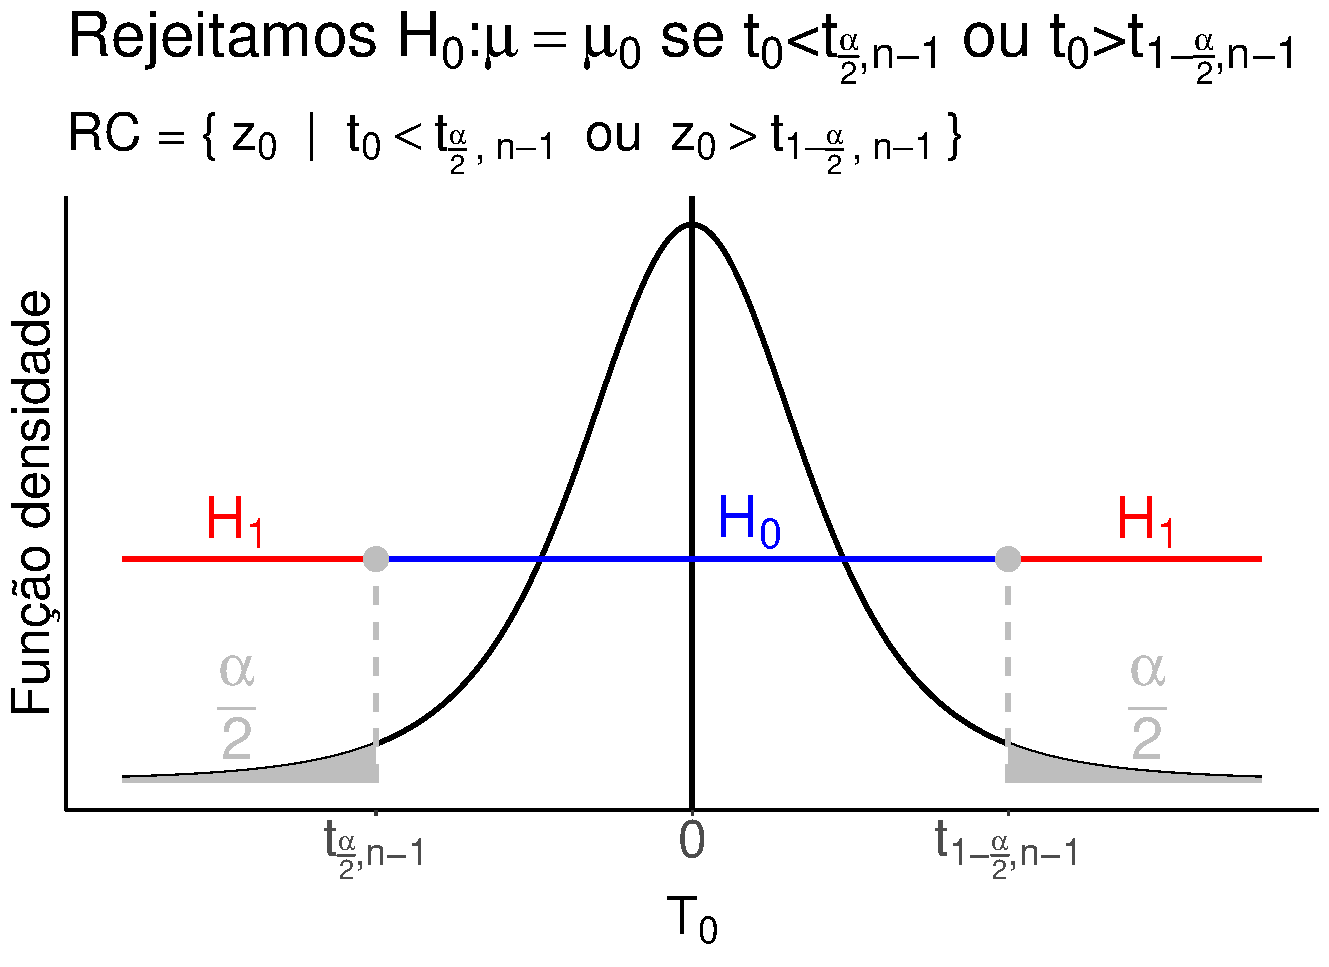
\includegraphics[width=0.32\linewidth]{figures/bilateral-normal-s2-unknown.pdf} \label{fig:bilateral-normal-s2-unknown}} \hfill
\subfloat[Teste unilateral.]{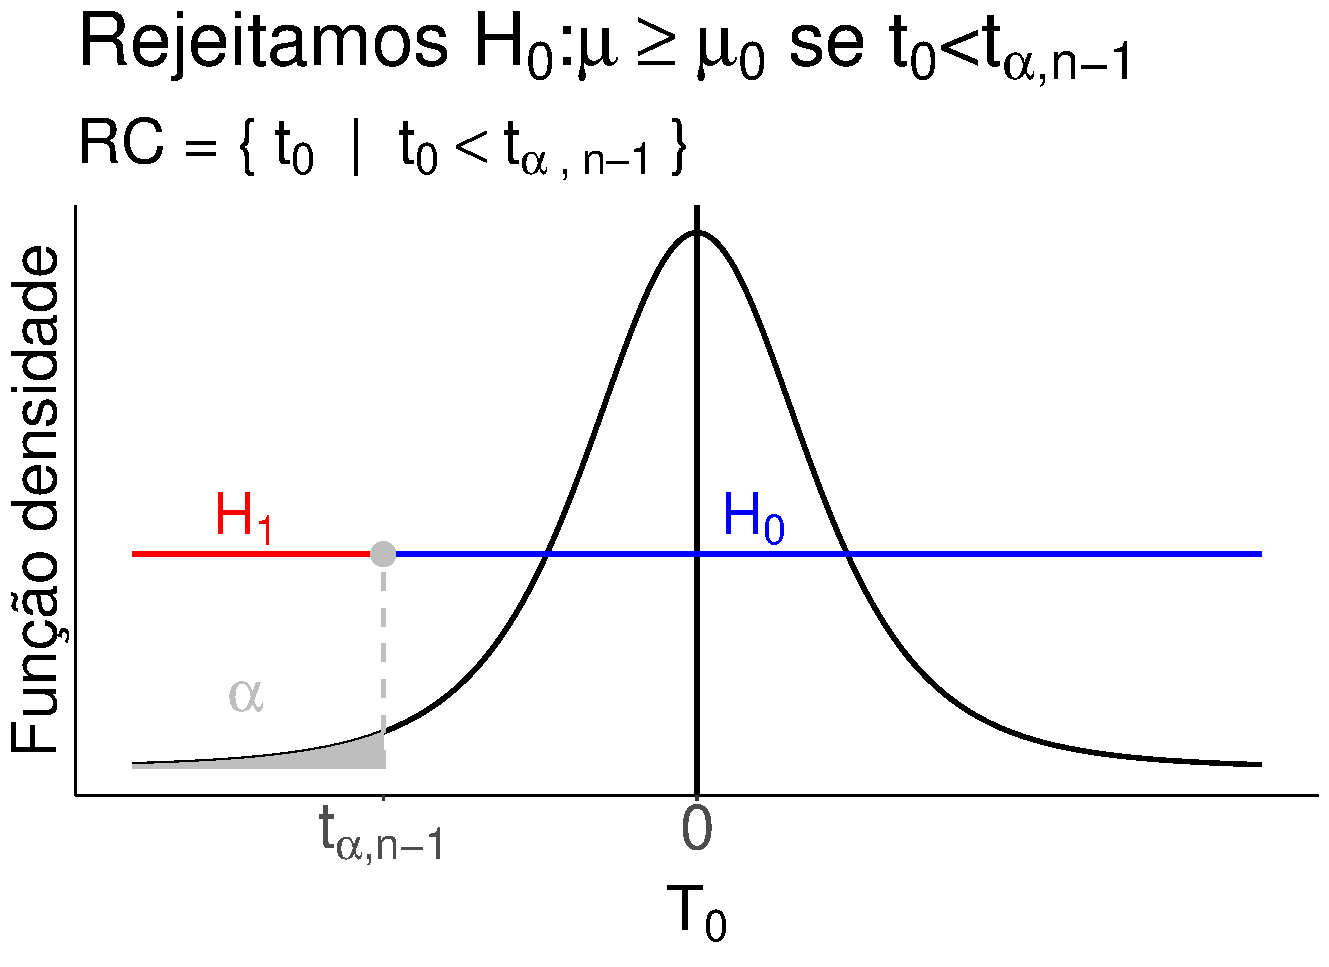
\includegraphics[width=0.32\linewidth]{figures/unilateral-h0-lower-normal-s2-unknown.pdf} \label{fig:unilateral-h0-lower-normal-s2-unknown}} \hfill
\subfloat[Teste unilateral.]{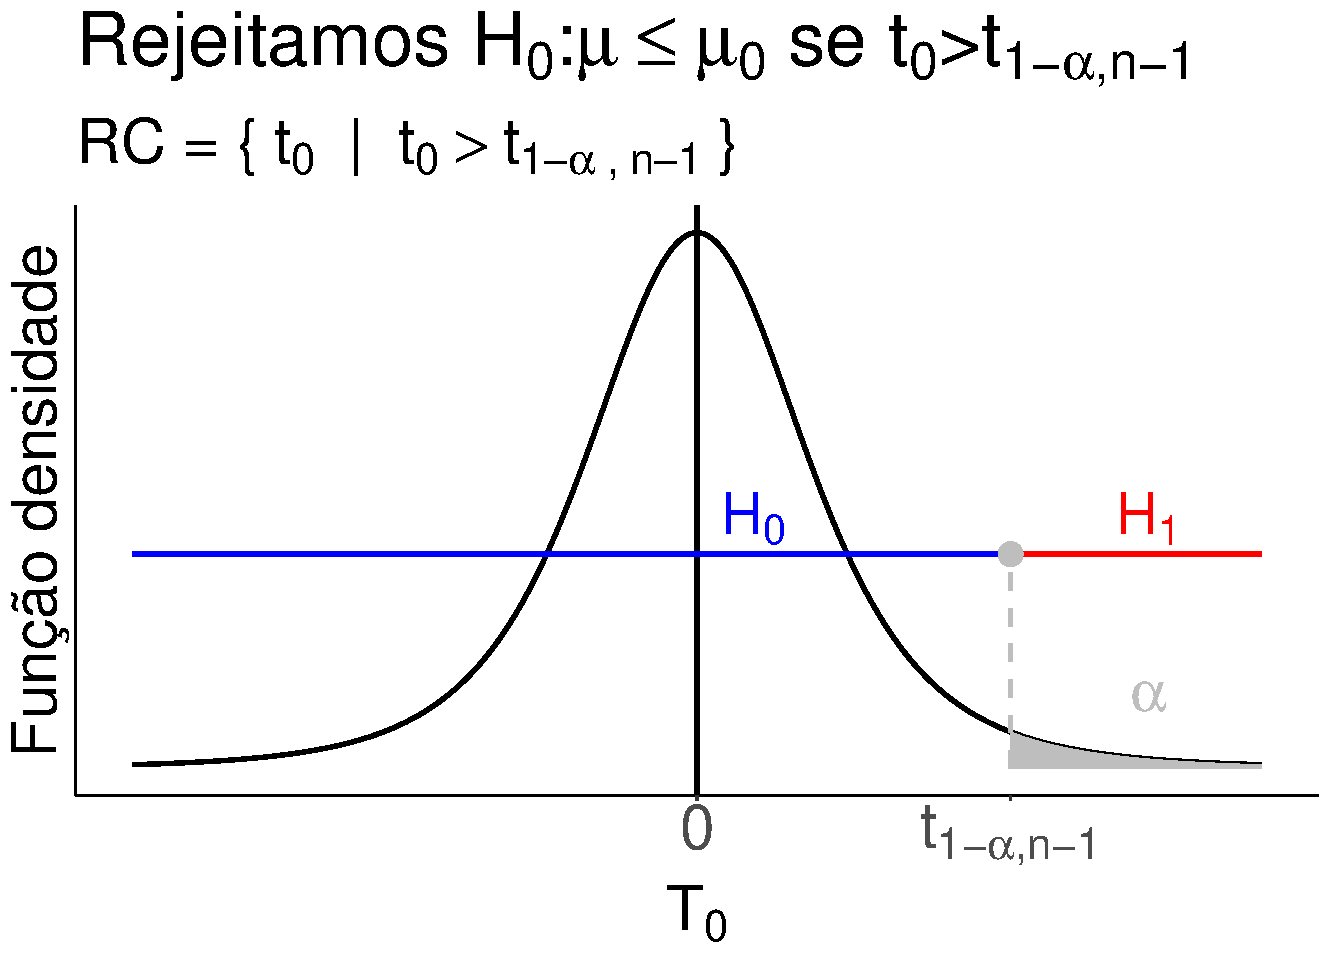
\includegraphics[width=0.32\linewidth]{figures/unilateral-h0-upper-normal-s2-unknown.pdf} \label{fig:unilateral-h0-upper-normal-s2-unknown}}
\caption{Região crítica para o teste t.}
\end{figure}


\normalsize

\end{frame}

\begin{frame}{Distribuição normal com $\sigma^2$ desconhecido (Teste t).}

\large
\begin{itemize}
	\item Na Figura~\ref{fig:bilateral-normal-s2-unknown}, testamos $H_0: \mu = \mu_0$ versus $H_1: \mu \neq \mu_0$. Rejeitamos $H_0$ se $t_0 = \frac{(\bar{x} - \mu_0)\sqrt{n}}{s} \in \allowbreak RC=\{t_0 \mid t_0 < t_{\frac{\alpha}{2}, n-1} \mbox{ ou } t_0 > t_{1-\frac{\alpha}{2}, n-1} \}$, em que $P\left(t_{n-1} \leq t_{\frac{\alpha}{2}, n-1} \right) = \frac{\alpha}{2}$ e $P\left(t_{n-1} \leq t_{1-\frac{\alpha}{2}, n-1} \right) = 1- \frac{\alpha}{2}$;
	\vfill
	
	\item Na Figura~\ref{fig:unilateral-h0-lower-normal-s2-unknown}, testamos $H_0: \mu \geq \mu_0$ versus $H_1: \mu < \mu_0$. Rejeitamos $H_0$ se $t_0 = \frac{(\bar{x} - \mu_0)\sqrt{n}}{s} \in \allowbreak RC=\{t_0 \mid t_0 < t_{\alpha, n-1}  \}$, em que $P\left(t_{n-1} \leq t_{\alpha} \right) =\alpha$;
	\vfill
	
	\item Na Figura~\ref{fig:unilateral-h0-upper-normal-s2-unknown}, testamos $H_0: \mu \leq \mu_0$ versus $H_1: \mu > \mu_0$. Rejeitamos $H_0$ se $t_0 = \frac{(\bar{x} - \mu_0)\sqrt{n}}{s} \in \allowbreak RC=\{t_0 \mid t_0 < t_{1-\alpha, n-1}  \}$, em que $P\left(t_{n-1} \leq t_{1-\alpha, n-1} \right) = 1-\alpha$.
\end{itemize}
Chamamos $t_{\alpha, n-1}$; $t_{1-\alpha, n-1}$; $t_{\frac{\alpha}{2}, n-1}$ e $t_{1-\frac{\alpha}{2}, n-1}$ de valores críticos.
\normalsize
\end{frame}

\begin{frame}{Distribuição normal com $\sigma^2$ desconhecido (Teste t).}

\large
\begin{block}{Exemplo}
	Deseja-se investigar se um certa moléstia, que ataca o rim, altera o consumo do oxigênio desse órgão. Para indivíduos sadios, admite-se que esse consumo tem distribuição normal com média $12cm^3/min$.
	Os valores medidos em cinco pacientes com a moléstia foram: 14,4; 12,9; 15,0; 13,7; e 13,5. Qual seria a conclusão, ao nível de significância de $1\%$?
\end{block}

\normalsize
\end{frame}

\begin{frame}{Distribuição normal com $\sigma^2$ desconhecido (Teste t).}

\begin{block}{Solução}
	\textbf{Passo 1)} Queremos testar as hipóteses: $H_0: \mu = \mu_0$ e $H_1: \mu \neq \mu_0$, em que $\mu_0=12$;
	
	\textbf{Passo 2)} Pelo enunciado, temos que o nível de significância é $\alpha=1\%$.
	
	\textbf{Passo 3)} Rejeitamos $H_0$ se $\lvert t_0 \rvert = \left\lvert \frac{(\bar{x} - \mu_0)\sqrt{n}}{s} \right\rvert$ for grande. Ou seja, $RC = \{ t_0 \mid t_0 < t_{\frac{\alpha}{2}, n-1} \mbox{ ou } t_0 > t_{1-\frac{\alpha}{2}, n-1} \}.$
	
	\textbf{Passo 4)} Vamos encontrar os valores críticos:
	\begin{itemize}
		\item $P\left( t_{n-1} \leq t_{\frac{\alpha}{2}, n-1} \right) = P\left( t_{4} \leq t_{0,005,4} \right) = \frac{\alpha}{2} = 0,005$, então $t_{0,005; 4} = -4,604$;
		\item $P\left( t_{n-1} \leq t_{1-\frac{\alpha}{2}, n-1} \right) = P\left( t_{4} \leq t_{0,995, 4} \right) = 1-\frac{\alpha}{2} = 0,995$, então $t_{0,995; 4} = 4,604$.
	\end{itemize}

	\textbf{Passo 5)} Note que $\bar{x} = 13,9$, $s = 0,82$ e $t_0 = \frac{(13,9 - 12)\sqrt{5}}{0,82} = 5,18$, então $t_0 \in RC$ e rejeitamos $H_0$. Ou seja, ao nível de significância $\alpha=1\%$, a moléstia altera o consumo de oxigênio.
\end{block}

\end{frame}

\begin{frame}{Distribuição normal com $\sigma^2$ desconhecido (Teste t).}

\begin{block}{Solução: p-valor (teste t bilateral)}
	O p-valor é calculado através da equação
	$$p=P\left( \left\lvert \frac{(\bar{X} - \mu_0)\sqrt{n}}{s} \right\rvert >  \left\lvert \frac{(\bar{x} - \mu_0)\sqrt{n}}{s}  \right\rvert \mid H_0 \right) = 2 \left[ 1 - P\left( t_{n-1} \leq \lvert t_0 \rvert \right) \right].$$
	
	Como $\bar{x} = 13,9$, $s=0,82$, $n=5$ e $t_0 = \frac{(\bar{x} -\mu_0)\sqrt{n}}{s} = 5,18$, então
	\begin{align*}
		p &= 2 \left[ 1 - P\left( t_{n-1} \leq \lvert t_0 \rvert \right) \right]\\
		&= 2 \left[ 1 - P\left( t_{4} \leq \lvert 5,18 \rvert \right) \right], \qquad \mbox{\textcolor{important}{Aqui precisamos usar o R ou MATLAB.}} \\
		&= 2 \left[ 1- 0.9967 \right]\\
		&= 0,0066.
	\end{align*}
	
	Como $p=0,0066 < 0,01 = \alpha$, ao nível de significância $1\%$, não rejeitamos $H_0$. Ou seja, ao nível de significância $1\%$, podemos afirmar que a moléstia altera o consumo de oxigênio pelo rim.
\end{block}

\end{frame}

\begin{frame}{Distribuição normal com $\sigma^2$ desconhecido (Teste t).}

\large
 \begin{block}{Exemplo}
	O crescimento de bebês, durante o primeiro mês de vida, pode ser modelado pela distribuição Normal. Admita que, em média, um crescimento de 5 centímetros ou mais seja considerado satisfatório. Deseja-se verificar se o crescimento de bebês de famílias em um bairro de periferia de São Paulo acompanha o padrão esperado ao nível de significância $\alpha=1\%$. Para tanto, 10 recém-nascidos na região foram sorteados e sua altura acompanhada, fornecendo as seguintes de crescimento em centímetros: 5,03; 5,02; 4,95; 4,96; 5,01; 4,97; 4,90; 4,91; 4,90 e 4,93.
\end{block}


\normalsize

\end{frame}

\begin{frame}{Distribuição normal com $\sigma^2$ desconhecido (Teste t).}

\large

\begin{block}{Solução}
	\textbf{Passo 1)} Queremos testar as hipóteses: $H_0: \mu \geq \mu_0$ e $H_1: \mu < \mu_0$, em que $\mu_0=5$;
	
	\textbf{Passo 2)} Pelo enunciado, o nível de significância é $\alpha=1\%$.
	
	\textbf{Passo 3)} Rejeitamos $H_0$ se $t_0= \frac{(\bar{x} - \mu_0)\sqrt{n}}{s}$ for pequeno. Ou seja, rejeitamos $H_0$ se $t_0 < t_{\alpha, n-1}$, em que $P\left( t_{n-1} \leq t_{\alpha, n-1} \right)=\alpha$. Então,
	$$RC = \{ t_0 \mid t_0 < t_{\alpha, n-1} \}.$$
	
	\textbf{Passo 4)} Vamos encontrar o valor crítico da região crítica:
	\begin{itemize}
		\item $P\left(t_{n-1} \leq t_{\alpha, n-1}\right) = P\left(t_{9} \leq t_{0,01, 9}\right)= \alpha = 0,01$, então $t_{0,01, 9} = -2,764$.
	\end{itemize}

	\textbf{Passo 5)} Note que $\bar{x}= 4,958$, $s=0,05$, $n-10$ e $t_0 = \frac{(\bar{x}- \mu_0)\sqrt{n}}{s} = -2,70$. Como $t_0 \not\in RC$, não rejeitamos $H_0$ ao nível de significância $\alpha=1\%$.
	
	Ao nível de significância $\alpha=1\%$, os bebês da periferia tem crescimento de, no mínimo, 5 centímetros.
\end{block}

\normalsize

\end{frame}

\begin{frame}{Distribuição normal com $\sigma^2$ desconhecido (Teste t).}

\large

\begin{block}{Solução (p-valor)}
	O p-valor é calculado através da equação
	$$p = P\left( \frac{(\bar{X} - \mu_0)\sqrt{n}}{s} < \frac{(\bar{x} - \mu_0)\sqrt{n}}{s} \mid H_0 \right) = P\left( t_{n-1} < t_0 \right).$$
	
	Como $\bar{x} = 4,958$, $s-0,05$, $n=10$ e $t_0 = \frac{(\bar{x} - \mu_0)\sqrt{n}}{s} = -2,70$, temos que
	\begin{align*}
		p &= P \left( t_{n-1} \leq t_0\right)\\
		&= P \left( t_9 \leq -2,70\right)\\
		&= 0,01.
	\end{align*}
	
	Como $p=0,01 \geq 0,01 = \alpha$, ao nível de significância $\alpha=1\%$, então não rejeitamos $H_0$, ou seja, o crescimentos dos bebês na periferia é, no mínimo, 5 centímetros.		
\end{block}

\normalsize

\end{frame}

\begin{frame}{Distribuição normal com $\sigma^2$ desconhecido (Teste t).}

\Large

\begin{block}{Exemplo}
	Imagine que um pesquisador tem uma amostra com 25 observações de uma variável aleatória com distribuição normal. Na Tabela~\ref{tab:normal-s2-unknown-unilateral-h0-upper}, apresentamos algumas informações para testar as hipóteses $H_0: \mu \leq 15$ e $H_1: \mu > 15$. Complete a Tabela~\ref{tab:normal-s2-unknown-unilateral-h0-upper}. Ao nível de significância $\alpha=5\%$, você rejeitaria $H_0$?
	\begin{table}[ht]
		\centering
		\begin{tabular}{c|c|c|c|c}
			\toprule[0.05cm]
			tamanho da amostra & $\bar{x}$ & $s$ & $t_0$ & valor-p \\ 
			\midrule
			25 & 20,69 & 2,10 &  &  \\ 
			\bottomrule[0.05cm]
		\end{tabular}
		\caption{Algumas informações do experimento.} 
		\label{tab:normal-s2-unknown-unilateral-h0-upper}
	\end{table}
\end{block}

\normalsize

\end{frame}

\begin{frame}{Distribuição normal com $\sigma^2$ desconhecido (Teste t).}

\large

\begin{block}{Solução (procedimento de Neymann-Pearson)}
	\textbf{Passo 1)} Pelo enunciado, temos as hipóteses: $H_0: \mu \leq \mu_0$ e $H_1: \mu > \mu_0$, em que $\mu_0 = 15$;
	
	\textbf{Passo 2)} Pelo enunciado, o nível de significância é $\alpha=5\%$.
	
	\textbf{Passo 3)} Rejeitamos $H_0$ se $t_0 = \frac{(\bar{x} -\mu_0)\sqrt{n}}{s}$ for grande. Ou seja, $RC = \{ t_0 \mid t_0 > t_{1-\alpha, n-1} \}.$
	\vfill
	
	\textbf{Passo 4)} Vamos calcular o valor crítico:
	\begin{itemize}
		\item $P\left( t_{n-1} < t_{1-\alpha, n-1} \right) = P\left( t_{24} < t_{0,95; 24} \right) = 1- \alpha = 0,95$, então $t_{0,95, 24} = 1,711$.
	\end{itemize}
	\vfill

	\textbf{Passo 5)} Note que $\bar{x} = 20,69$, $s=2,10$ e $n=25$, então $t_0 = \frac{(20,69 - 15)\sqrt{25}}{2,10}=13,55$ e $t_0 \in RC$, ou seja, rejeitamos $H_0$ ao nível de significância $5\%$. 
\end{block}
\normalsize
\end{frame}

\begin{frame}{Distribuição normal com $\sigma^2$ desconhecido (Teste t).}

\normalsize

\begin{block}{Solução (p-valor)}
	O valor-p é calculado através da equação
	$$p = P\left( \frac{(\bar{X} - \mu_0)\sqrt{n}}{s} > \frac{(\bar{x} - \mu_0)\sqrt{n}}{s} \right) = 1 - P \left( t_{n-1} \leq \frac{(\bar{x} - \mu_0)\sqrt{n}}{s} \right)= 1- P(t_{n-1} \leq t_0).$$
	
	Como $\bar{x}=20,69$, $s=2,10$, $n=25$ e $t_0=13,55$, temos que
	\begin{align*}
		p &=1- P\left( t_{n-1} \leq t_0  \right)\\
		&=1- P \left( t_{24} \leq 13,55 \right)\qquad \mbox{\textcolor{important}{Aqui precisamos usar o R ou MATLAB.}}\\
		&=1 - 1\\
		&= 0.
	\end{align*}
	
	Como $p=0 < 0,05=\alpha$, ao nível de significância $\alpha=5\%$ rejeitamos $H_0$.
\end{block}

\normalsize
\end{frame}

\subsection{Poder e tamanho da amostra.}

\begin{frame}{Poder do teste: $H_0:\mu = \mu_0$ e $H_1: \mu \neq \mu_0$.}

\scriptsize

Imagine que
\begin{itemize}
	\item Hipóteses: $H_0: \mu = \mu_0$ e $H_1: \mu \neq \mu_0$;
	\item $H_1$ é verdade e $\mu = \mu_0 + \delta$;
	\item $T_0 = \frac{(\bar{X} - \mu_0)\sqrt{n}}{s}  \sim t_{n-1}\left( \frac{\delta \sqrt{n}}{\sigma} \right)$;
	\item $t_{n-1}\left(\frac{\delta\sqrt{n}}{\sigma}\right)$ é  a distribuição t-Student com $n-1$ graus de liberdade e parâmetro de não-centralidade $\frac{\delta \sqrt{n}}{\sigma}$;
	\item Ao nível de significância $\alpha$, temos $RC = \{ t_0 \mid t_0 < t_{\frac{\alpha}{2}, n-1} \mbox{ ou } t_{1-\frac{\alpha}{2}, n-1} < t_0   \}$;
	\item Chamamos $\frac{\delta}{\sigma}$ é tamanho do efeito ou \textit{effect size}.
\end{itemize}
\vfill	

Poder do teste é dado
\begin{align*}
\textcolor{important}{1-\beta} &=1 - \left[P\left( t_{\frac{\alpha}{2}, n-1} \leq T_0 \leq t_{1-\frac{\alpha}{2}, n-1} \mid \mu = \mu_0 + \delta \right)\right]  \\
&= 1- P\left( T_0 \leq t_{1-\frac{\alpha}{2}, n-1} \mid \mu = \mu_0 + \delta \right) + P\left( T_0 \leq t_{\frac{\alpha}{2}, n-1} \mid \mu = \mu_0 + \delta \right)\\
&= 1 - P\left( t_{n-1}\left(\frac{\delta\sqrt{n}}{\sigma}\right) \leq t_{1-\frac{\alpha}{2}, n-1} \right) + P\left( t_{n-1}\left(\frac{\delta\sqrt{n}}{\sigma}\right) \leq t_{\frac{\alpha}{2}, n-1} \right),
\end{align*}
\vfill

A \textcolor{important}{Função Poder}, dado o tamanho da amostra $n$, é uma função das médias populacionais na hipótese alternativa  $\pi: \mathbb{R}-\{0\} \longrightarrow [0,1]$ dada por
\begin{align*}
\pi(\delta) =  1 - P\left( t_{n-1}\left(\frac{\delta\sqrt{n}}{\sigma}\right) \leq t_{1-\frac{\alpha}{2}, n-1} \right) + P\left( t_{n-1}\left(\frac{\delta\sqrt{n}}{\sigma}\right) \leq t_{\frac{\alpha}{2}, n-1} \right), \delta = \mu - \mu_0, \delta \in \mathbb{R} - \{0 \}.
\end{align*}
Alguns livros chamada a Função Poder de \textcolor{important}{Curva de Característica Operacional.}

\normalsize	
\end{frame}

\begin{frame}{Tamanho do teste: $H_0:\mu = \mu_0$ e $H_1: \mu \neq \mu_0$.}

\small

Imagine que
\begin{itemize}
	\item Hipóteses: $H_0: \mu = \mu_0$ e $H_1: \mu \neq \mu_0$;
	\item $H_1$ é verdade e $\mu = \mu_0 + \delta$;
	\item $T_0 = \frac{(\bar{X} - \mu_0)\sqrt{n}}{s}  \sim t_{n-1}\left( \frac{\delta \sqrt{n}}{\sigma} \right)$;
	\item $t_{n-1}\left(\frac{\delta\sqrt{n}}{\sigma}\right)$ é a distribuição t-Student com $n-1$ graus de liberdade e $\mu=\frac{\delta \sqrt{n}}{\sigma}$ é o parâmetro de não-centralidade;
	\item Ao nível de significância $\alpha$, temos $RC = \{ t_0 \mid t_{\frac{\alpha}{2}, n-1} \leq t_0 \leq t_{1-\frac{\alpha}{2}, n-1}   \}$;
	\item Chamamos $\frac{\delta}{\sigma}$ de tamanho do efeito ou \textit{effect size};
\end{itemize}
\vfill

Dado o poder do teste $1-\beta$ (e o erro $\beta$), nível de significância $\alpha$, o tamanho do efeito $\frac{\delta}{\sigma}$, então encontramos o tamanho da amostra resolvendo a seguinte equação:
\begin{align}\label{eq:sample-size-s2-unknown-bilateral}
	1-\beta =1- P\left( t_{n-1}\left(\frac{\delta \sqrt{n}}{\sigma}\right) \leq t_{1-\frac{\alpha}{2}, n-1}  \right) + P\left( t_{n-1}\left(\frac{\delta \sqrt{n}}{\sigma}\right) \leq t_{\frac{\alpha}{2}, n-1}  \right)
\end{align}

A equação~\eqref{eq:sample-size-s2-unknown-bilateral} é resolvida usando métodos numéricos. Tais métodos são estão implementados em diversos \textit{softwares}:
\begin{description}
	\item[No R] \lstinline|pwr_t_test_1pop|.
\end{description}

Esta função está no pacote \lstinline|power|, que pode ser instalado usando o pacote \lstinline|devtools|: \lstinline|devtools::install_github("gilberto-sassi/power")|.

\normalsize

\end{frame}

\begin{frame}{Poder do teste: $H_0:\mu = \mu_0$ e $H_1: \mu \neq \mu_0$.}

\large
\begin{block}{Exemplo}
	Deseja-se investigar se um certa moléstia, que ataca o rim, altera o consumo do oxigênio desse órgão. Para indivíduos sadios, admite-se que esse consumo tem distribuição normal com média $12cm^3/min$ para pacientes sadios.
	Cinco pacientes com a moléstia tiveram o consumo de oxigênio no rim mensurado. Se a média e o desvio padrão populacional de consumo de oxigênio de pessoas com esta moléstia são, respectivamente, $\mu=16cm^3/\min$ e $\sigma=2$, qual o poder do teste ao nível de significância de $1\%$?
\end{block}
\normalsize

\end{frame}

\begin{frame}[fragile]{Poder do teste: $H_0:\mu = \mu_0$ e $H_1: \mu \neq \mu_0$.}

\small

\begin{block}{Solução}
	\textbf{Passo 1)} Querer testar as seguintes hipóteses: $H_0: \mu = \mu_0$ e $H_1: \mu \neq \mu_0$, em que $\mu_0=12$;
	
	\textbf{Passo 2)} Nível de significância $\alpha=1\%$.
	
	
	Note que $\mu=16=\mu_0+\delta=12+\delta$, $\delta=4$, $\alpha=0,01$, $\sigma=2$, $n=5$ e $\frac{\delta}{\sigma} = \frac{4}{2}=2$.
	
	Vamos encontrar os quantis da distribuição $t$-Student:
	\begin{itemize}
		\item $P(t_{n-1} \leq t_{\frac{\alpha}{2}, n-1} ) = P(t_{4} \leq t_{0,005; 4} ) = \frac{\alpha}{2} = 0,005$, então $t_{0,005; 4}=-4,604$;
		\item $P(t_{n-1} \leq t_{1-\frac{\alpha}{2}, n-1} ) = P(t_{4} \leq t_{0,995; 4} ) =1- \frac{\alpha}{2} = 0,995$, então $t_{0,995; 4}=4,604$.
	\end{itemize}
	
	Então o poder do teste é dado por
	\begin{align*}
		1-\beta &= 1 - P\left( t_{n-1}\left(\frac{\delta\sqrt{n}}{\sigma}\right) \leq t_{1-\frac{\alpha}{2}, n-1} \right) + P\left( t_{n-1}\left(\frac{\delta\sqrt{n}}{\sigma}\right) \leq t_{\frac{\alpha}{2}, n-1} \right)\\
		&= 1 - P\left( t_{4}\left(\frac{4\sqrt{5}}{2}\right) \leq t_{0,995, 4} \right) + P\left( t_{4}\left(\frac{4\sqrt{5}}{2}\right) \leq t_{0,005, 4} \right)\\
		&= 1 - P\left( t_{4}\left(\frac{4\sqrt{5}}{2}\right) \leq 4,604 \right) + P\left( t_{4}\left(\frac{4\sqrt{5}}{2}\right) \leq -4,604 \right)\\
		&= 0,5472.
	\end{align*} 
\end{block}

\begin{lstlisting}[language = C, caption = Código no R.]
pwr_t_test_1pop(m = 16, m0 = 12, sigma = 2, n = 5, pwr = NULL,
		alternative = "two.sided", sig_level = 0.01)
\end{lstlisting}
\normalsize


\end{frame}


\begin{frame}{Tamanho da amostra: $H_0:\mu = \mu_0$ e $H_1: \mu \neq \mu_0$.}

\large
\begin{block}{Exemplo}
	Deseja-se investigar se um certa moléstia, que ataca o rim, altera o consumo do oxigênio desse órgão. Para indivíduos sadios, admite-se que esse consumo tem distribuição normal com média $12cm^3/min$ para pacientes sadios.
	Cinco pacientes com a moléstia tiveram o consumo de oxigênio no rim mensurado. Se a média e o desvio padrão populacional de consumo de oxigênio de pessoas com esta moléstia são, respectivamente, $\mu=16cm^3/\min$ e $\sigma=2$, qual o tamanho \sout{mínimo} de amostra para termos um poder de teste de $95\%$ ao nível de significância de $1\%$?
\end{block}
\normalsize

\end{frame}

\begin{frame}[fragile]{Tamanho da amostra: $H_0:\mu = \mu_0$ e $H_1: \mu \neq \mu_0$.}


\begin{block}{Solução}
	\textbf{Passo 1)} Querer testar as seguintes hipóteses: $H_0: \mu = \mu_0$ e $H_1: \mu \neq \mu_0$, em que 	em que $\mu_0=12$;

	
	\textbf{Passo 2)} Nível de significância $\alpha=1\%$.

	
	Como $\mu=16=\mu_0+\delta=12+\delta$, $\delta=4$, $\alpha=0,01$, $\sigma=2$, $1-\beta=0.95$ e $\frac{\delta}{\sigma} = \frac{4}{2}=2$.
	
	Primeiro vamos encontrar os quantis da distribuição $t$-Student:
	\begin{itemize}
		\item $P(t_{n-1} \leq t_{\frac{\alpha}{2}, n-1} ) = P(t_{4} \leq t_{0,005; 4} ) = \frac{\alpha}{2} = 0,005$, então $t_{0,005; 4}=-4,604$;
		\item $P(t_{n-1} \leq t_{1-\frac{\alpha}{2}, n-1} ) = P(t_{4} \leq t_{0,995; 4} ) =1- \frac{\alpha}{2} = 0,995$, então $t_{0,995; 4}=4,604$.
	\end{itemize}
	
	Então o tamanho da amostra é solução em $n$ da seguinte equação
	\begin{align*}
	0,95 &= 1 - P\left( t_{n-1}\left(\frac{\delta\sqrt{n}}{\sigma}\right) \leq t_{1-\frac{\alpha}{2}, n-1} \right) + P\left( t_{n-1}\left(\frac{\delta\sqrt{n}}{\sigma}\right) \leq t_{\frac{\alpha}{2}, n-1} \right)
	\end{align*} 
\end{block}
Então, precisamos analisar o consumo de oxigênio nos rins em $n=8$ pacientes com moléstia.

Código do \lstinline|R|:
\begin{lstlisting}[caption = Código no R., language = C]
pwr_t_test_1pop(m = 16, m0 = 12, sigma = 2, n = NULL, pwr = 0.95,
		alternative = "two.sided", sig_level = 0.01)
\end{lstlisting}

\end{frame}

%\begin{frame}{Tamanho da amostra: $H_0:\mu = \mu_0$ e $H_1: \mu \neq \mu_0$.}
%
%\begin{figure}[htbp]
%	\centering
%	\caption{Cálculo do tamanho da amostra no \texttt{R}.}
%	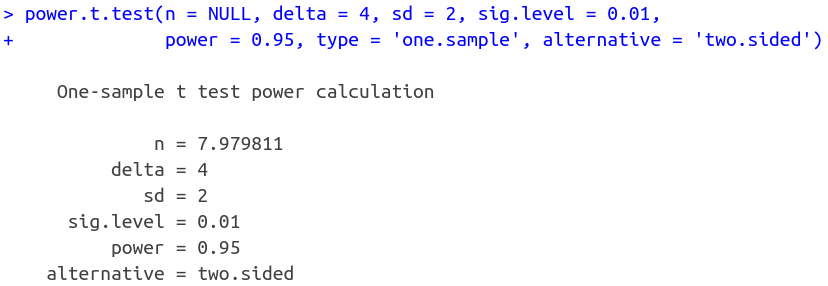
\includegraphics[width=0.9\linewidth]{figures/t-noncentral-sample-size-R.png}
%\end{figure}
%
%\end{frame}

\begin{frame}{Poder do teste: $H_0:\mu \geq \mu_0$ e $H_1: \mu < \mu_0$.}

\small

Imagine que
\begin{itemize}
	\item Hipóteses: $H_0: \mu \geq \mu_0$ e $H_1: \mu < \mu_0$;
	\item $H_1$ é verdade e $\mu = \mu_0 + \delta$, em que $\delta < 0$;
	\item $T_0 = \frac{(\bar{X} - \mu_0)\sqrt{n}}{s}  \sim t_{n-1}\left( \frac{\delta \sqrt{n}}{\sigma} \right)$;
	\item $t_{n-1}\left(\frac{\delta\sqrt{n}}{\sigma}\right)$ é  a distribuição t-Student com $n-1$ graus de liberdade e parâmetro de não-centralidade $\mu = \frac{\delta \sqrt{n}}{\sigma}$;
	\item Ao nível de significância $\alpha$, temos $RC = \{ t_0 \mid t_0 < t_{\alpha, n-1}   \}$;
	\item Chamamos $\frac{\delta}{\sigma}$ é tamanho do efeito ou \textit{effect size}.
\end{itemize}
\vfill	

Poder do teste é dado
\begin{align*}
\textcolor{important}{1-\beta} &=1 - \left[P\left( T_0 \geq t_{\alpha, n-1} \mid \mu = \mu_0 + \delta \right)\right]  = P\left( t_{n-1}\left( \frac{\delta\sqrt{n}}{\sigma} \right) \leq t_{\alpha, n-1} \right).
\end{align*}
\vfill

A \textcolor{important}{Função Poder}, dado o tamanho da amostra $n$, é uma função das médias populacionais na hipótese alternativa  $\pi: (-\infty, 0) \longrightarrow [0,1]$ dada por
\begin{align*}
\pi(\delta) =  P\left( t_{n-1}\left( \frac{\delta\sqrt{n}}{\sigma} \right) \leq t_{\alpha, n-1}  \right),\qquad \delta = \mu - \mu_0, \delta \in (-\infty, 0).
\end{align*}
Alguns livros chamada a Função Poder de \textcolor{important}{Curva de Característica Operacional.}

\normalsize	

\end{frame}

\begin{frame}{Tamanho do teste: $H_0:\mu \geq \mu_0$ e $H_1: \mu < \mu_0$.}

\normalsize

Imagine que
\begin{itemize}
	\item Hipóteses: $H_0: \mu \geq \mu_0$ e $H_1: \mu < \mu_0$;
	\item $H_1$ é verdade e $\mu = \mu_0 + \delta$, em que $\delta < 0$;
	\item $T_0 = \frac{(\bar{X} - \mu_0)\sqrt{n}}{s}  \sim t_{n-1}\left( \frac{\delta \sqrt{n}}{\sigma} \right)$;
	\item $t_{n-1}\left(\frac{\delta\sqrt{n}}{\sigma}\right)$ é a distribuição t-Student com $n-1$ graus de liberdade e $\mu=\frac{\delta \sqrt{n}}{\sigma}$ é o parâmetro de não-centralidade;
	\item Ao nível de significância $\alpha$, temos $RC = \{ t_0 \mid t_0 < t_{\alpha, n-1}   \}$;
	\item Chamamos $\frac{\delta}{\sigma}$ de tamanho do efeito ou \textit{effect size};
\end{itemize}
\vfill

Dado o poder do teste $1-\beta$ (e o erro $\beta$), nível de significância $\alpha$, o tamanho do efeito $\frac{\delta}{\sigma}$, então encontramos o tamanho da amostra resolvendo a seguinte equação:
\begin{align}\label{eq:sample-size-s2-unknown-unilateral-upper}
\beta = 1- P\left( t_{n-1}\left( \frac{\delta\sqrt{n}}{\sigma}\right) \leq t_{\alpha, n-1}  \right)
\end{align}

A equação~\eqref{eq:sample-size-s2-unknown-unilateral-upper} é resolvida usando métodos numéricos. Tais métodos são estão implementados em diversos \textit{softwares}:
\begin{description}
	\item[No R] \lstinline|pwr_t_test_1pop|.
\end{description}

Esta função está no pacote \lstinline|power|, que pode ser instalado usando o pacote \lstinline|devtools|: \lstinline|devtools::install_github("gilberto-sassi/power")|.

\normalsize

\end{frame}

\begin{frame}{Poder do teste: $H_0:\mu \geq \mu_0$ e $H_1: \mu < \mu_0$.}

\large
\begin{block}{Exemplo}
	O crescimento de bebês, durante o primeiro mês de vida, pode ser modelado pela distribuição Normal. Admita que, em média, um crescimento de 5 centímetros ou mais seja considerado satisfatório. Deseja-se verificar se o crescimento de bebês de famílias em um bairro de periferia de São Paulo acompanha o padrão esperado ao nível de significância $\alpha=1\%$. Para tanto, 10 recém-nascidos na região foram sorteados e sua altura acompanhada. Se a média e o desvio padrão populacional do crescimento de bebês na periferia são, respectivamente, $\mu=3$ centímetros e $\sigma=2$ centímetros, qual o poder do teste ao nível de significância $\alpha=5\%$?
\end{block}
\normalsize

\end{frame}

\begin{frame}[fragile]{Poder do teste: $H_0:\mu \geq \mu_0$ e $H_1: \mu < \mu_0$.}

\normalsize

\begin{block}{Solução}
	\textbf{Passo 1)} Queremos testar as seguintes hipóteses: $H_0: \mu \geq \mu_0$ e $H_1: \mu < \mu_0$, em que $\mu_0=5$;
	
	\textbf{Passo 2)} Nível de significância $\alpha = 5\%$;
	
	
	Note que $\mu=3=\mu_0 + \delta = 5 + \delta$, $\delta = -2$, $\sigma = 2$, $n=20$ e $\alpha=0,05$.
	
	Primeiro vamos encontrar o quantil da distribuição $t$-Student:
	\begin{itemize}
		\item $P\left( t_{n-1} \leq t_{\alpha, n-1} \right) = P\left( t_9 \leq t_{0,05; 9} \right) = \alpha = 0,05$, então $t_{0,05; 9} = -1,833$.
	\end{itemize}
	
	Então o poder do teste é dado por
	\begin{align*}
		1-\beta &= P \left( t_{n-1}\left( \frac{\delta\sqrt{n}}{\sigma}\right) \leq t_{\alpha, n-1}  \right) = P \left( t_{9}\left( \frac{-2\sqrt{10}}{2}\right) \leq t_{0,05;, 9} \right) \\ 
		&= P \left( t_{9}\left( \frac{-2\sqrt{10}}{2}\right) \leq -1,833 \right) = 0,8975.
	\end{align*}
\end{block}

\begin{lstlisting}[language = C, caption = Código no R.]
pwr_t_test_1pop(m = 3, m0 = 5, sigma = 2, n = 10, pwr = NULL,
		alternative = "less", sig_level = 0.05)
\end{lstlisting}

\normalsize

\end{frame}

\begin{frame}{Tamanho da amostra: $H_0:\mu \geq \mu_0$ e $H_1: \mu < \mu_0$.}

\large

\begin{block}{Exemplo}
	O crescimento de bebês, durante o primeiro mês de vida, pode ser modelado pela distribuição Normal. Admita que, em média, um crescimento de 5 centímetros ou mais seja considerado satisfatório. Deseja-se verificar se o crescimento de bebês de famílias em um bairro de periferia de São Paulo acompanha o padrão esperado ao nível de significância $\alpha=1\%$. Para tanto, 10 recém-nascidos na região foram sorteados e sua altura acompanhada. Se a média e o desvio padrão populacional do crescimento de bebês na periferia são, respectivamente, $\mu=3$ centímetros e $\sigma=2$ centímetros, quantos bebês o pesquisador precisa acompanhar para ter o poder do teste $95\%$?
\end{block}

\normalsize

\end{frame}



\begin{frame}[fragile]{Tamanho da amostra: $H_0:\mu \geq \mu_0$ e $H_1: \mu < \mu_0$.}


\begin{block}{Solução}
	\textbf{Passo 1)} Queremos testar as seguintes hipóteses: $H_0: \mu \geq \mu_0$ e $H_1: \mu < \mu_0$, em que $\mu_0=5$;

	\textbf{Passo 2)} Nível de significância $\alpha = 5\%$;
	
	Note que $\mu=3=\mu_0+\delta=5+\delta$, $\delta=-2$, $\alpha=0,05$, $\sigma=2$, $1-\beta=0.95$ e $\frac{\delta}{\sigma} = \frac{-2}{2}=-1$.
	
	Primeiro vamos calcular o quantil da distribuição $t$-Student:
	\begin{itemize}
		\item $P\left( t_{n-1} \leq t_{\alpha, n-1} \right) = P\left( t_9 \leq t_{0,05; 9} \right) = \alpha = 0,05$, então $t_{0,05; 9} = -1,833$.
	\end{itemize}
	
	Então o tamanho da amostra é solução em $n$ da seguinte equação
	\begin{align*}
	0,05 &= P\left( t_{n-1}\left(\frac{\delta\sqrt{n}}{\sigma}\right) \leq t_{1-\alpha, n-1} \right) = P \left( t_{n-1}\left( \frac{-2\sqrt{10}}{2} \right) \leq -1,833 \right)
	\end{align*} 
\end{block}
Então, precisamos acompanhar $n=13$ bebês da periferia.

\begin{lstlisting}[language = C, caption = Código no R.]
pwr_t_test_1pop(m = 3, m0 = 5, sigma = 2, n = NULL, pwr = 0.95, alternative = "less", sig_level = 0.05)
\end{lstlisting}

\end{frame}

\begin{frame}{Poder do teste: $H_0:\mu \leq \mu_0$ e $H_1: \mu > \mu_0$.}

\small

Imagine que
\begin{itemize}
	\item Hipóteses: $H_0: \mu \leq \mu_0$ e $H_1: \mu > \mu_0$;
	\item $H_1$ é verdade e $\mu = \mu_0 + \delta$, em que $\delta > 0$;
	\item $T_0 = \frac{(\bar{X} - \mu_0)\sqrt{n}}{s}  \sim t_{n-1}\left( \frac{\delta \sqrt{n}}{\sigma} \right)$;
	\item $t_{n-1}\left(\frac{\delta\sqrt{n}}{\sigma}\right)$ é  a distribuição t-Student com $n-1$ graus de liberdade e parâmetro de não-centralidade $\mu = \frac{\delta \sqrt{n}}{\sigma}$;
	\item Ao nível de significância $\alpha$, temos $RC = \{ t_0 \mid t_0 > t_{1-\alpha, n-1}   \}$;
	\item Chamamos $\frac{\delta}{\sigma}$ é tamanho do efeito ou \textit{effect size}.
\end{itemize}
\vfill	

Poder do teste é dado
\begin{align*}
\textcolor{important}{1-\beta} &=1 - \left[P\left( T_0 \leq t_{1-\alpha, n-1} \mid \mu = \mu_0 + \delta \right)\right]  = 1- P\left( t_{n-1}\left( \frac{\delta\sqrt{n}}{\sigma} \right) \leq t_{1-\alpha, n-1}  \right).
\end{align*}
\vfill

A \textcolor{important}{Função Poder}, dado o tamanho da amostra $n$, é uma função das médias populacionais na hipótese alternativa  $\pi: (0, \infty) \longrightarrow [0,1]$ dada por
\begin{align*}
\pi(\delta) = 1 -  P\left( t_{n-1}\left( \frac{\delta\sqrt{n}}{\sigma} \right) \leq t_{1-\alpha, n-1} \right),\qquad \delta = \mu - \mu_0, \delta \in (0, \infty).
\end{align*}
Alguns livros chamada a Função Poder de \textcolor{important}{Curva de Característica Operacional.}

\normalsize	

\end{frame}

\begin{frame}{Tamanho do teste: $H_0:\mu \leq \mu_0$ e $H_1: \mu > \mu_0$.}

\small

Imagine que
\begin{itemize}
\item Hipóteses: $H_0: \mu \leq \mu_0$ e $H_1: \mu > \mu_0$;
\item $H_1$ é verdade e $\mu = \mu_0 + \delta$, em que $\delta > 0$;
\item $T_0 = \frac{(\bar{X} - \mu_0)\sqrt{n}}{s}  \sim t_{n-1}\left( \frac{\delta \sqrt{n}}{\sigma} \right)$;
\item $t_{n-1}\left(\frac{\delta\sqrt{n}}{\sigma}\right)$ é a distribuição t-Student com $n-1$ graus de liberdade e $\mu=\frac{\delta \sqrt{n}}{\sigma}$ é o parâmetro de não-centralidade;
\item Ao nível de significância $\alpha$, temos $RC = \{ t_0 \mid t_0 > t_{1-\alpha, n-1}   \}$;
\item Chamamos $\frac{\delta}{\sigma}$ de tamanho do efeito ou \textit{effect size};
\end{itemize}
\vfill

Dado o poder do teste $1-\beta$ (e o erro $\beta$), nível de significância $\alpha$, o tamanho do efeito $\frac{\delta}{\sigma}$, então encontramos o tamanho da amostra resolvendo a seguinte equação:
\begin{align}\label{eq:sample-size-s2-unknown-unilateral-lower}
\beta = P\left( t_{n-1}\left( \frac{\delta\sqrt{n}}{\sigma}\right) \leq t_{1-\alpha, n-1}  \right)
\end{align}

A equação~\eqref{eq:sample-size-s2-unknown-unilateral-lower} é resolvida usando métodos numéricos. Tais métodos são estão implementados em diversos \textit{softwares}:
\begin{description}
\item[No R] \lstinline|pwr_t_test_1pop|
\end{description}

Esta função está no pacote \lstinline|power|, que pode ser instalado usando o pacote \lstinline|devtools|: \lstinline|devtools::install_github("gilberto-sassi/power")|.

\normalsize

\end{frame}

\begin{frame}{Poder do teste: $H_0:\mu \leq \mu_0$ e $H_1: \mu > \mu_0$.}

\large

\begin{block}{Exemplo}
	Imagine que um pesquisador tem uma amostra com 25 observações de uma variável aleatória com distribuição normal. Na Tabela~\ref{tab:normal-s2-unknown-unilateral-h0-lower}, apresentamos algumas informações para testar as hipóteses $H_0: \mu \leq 15$ e $H_1: \mu > 15$. Complete a Tabela~\ref{tab:normal-s2-unknown-unilateral-h0-lower} usando o nível de significância $\alpha=5\%$. Assuma que a média e desvio padrão populacional são, respectivamente, $\mu=20$ e $\sigma=1.5$?
	\begin{table}[ht]
		\centering
		\scalebox{0.8}{
		\begin{tabular}{c|c|c|c|c|c}
			\toprule[0.05cm]
			tamanho da amostra & $\bar{x}$ & $s$  &  $\delta$ & tamanho do efeito & Poder do teste\\ 
			\midrule
			25 & 20,69 & 2,10 &  & &  \\ 
			\bottomrule[0.05cm]
		\end{tabular}
		}
		\caption{Algumas informações do experimento.} 
		\label{tab:normal-s2-unknown-unilateral-h0-lower}
	\end{table}
\end{block}

\normalsize

\end{frame}

\begin{frame}[fragile]{Poder do teste: $H_0:\mu \leq \mu_0$ e $H_1: \mu > \mu_0$.}

\begin{block}{Solução}
	\textbf{Passo 1)} Do enunciado, sabemos que queremos testar as hipóteses: $H_0: \mu \leq \mu_0$ e $H_1: \mu > \mu_0$;

	\textbf{Passo 2)} Nível de significância $\alpha = 5\%$;
	
	Como $\mu=20=\mu_0 + \delta = 15 + \delta$, $\delta = 5$, $\sigma = 1.5$, $n=25$ e $\alpha=0,05$.
	
	Primeiro vamos encontrar o quantil da distribuição $t$-Student:
	\begin{itemize}
		\item $P\left( t_{n-1} \leq  t_{1-\alpha, n-1} \right) = P\left( t_{24} \leq  t_{0,95, 24} \right) = 1-\alpha = 0,95$, então $t_{0,95; 24} = 1,711$.
	\end{itemize}
	
	Então o poder do teste é dado por
	\begin{align*}
	\beta &= P \left( t_{n-1}\left( \frac{\delta\sqrt{n}}{\sigma}\right) \leq t_{1-\alpha, n-1}  \right) = P \left( t_{24}\left( \frac{5\sqrt{25}}{1.5}\right) \leq t_{0,95;, 24} \right) \\ 
	&= P \left( t_{24}\left( \frac{5\sqrt{25}}{1.5}\right) \leq 1,711 \right) = 1.
	\end{align*}
\end{block}

\begin{lstlisting}[language = C, caption = Código no R.]
pwr_t_test_1pop(m = 20, m0 = 15, sigma = 1.5, n = 25, pwr = NULL,
		alternative = "greater", sig_level = 0.05)
\end{lstlisting}
\end{frame}


\begin{frame}{Tamanho da amostra: $H_0:\mu \leq \mu_0$ e $H_1: \mu > \mu_0$.}

\normalsize

\begin{block}{Exemplo}
		Imagine que um pesquisador tem uma amostra com 25 observações de uma variável aleatória com distribuição. Na Tabela~\ref{tab:normal-s2-unknown-unilateral-h0-upper-power}, apresentamos algumas informações para testar as hipóteses $H_0: \mu \leq 15$ e $H_1: \mu > 15$. Complete a Tabela~\ref{tab:normal-s2-unknown-unilateral-h0-upper-power} usando o nível de significância $\alpha=5\%$ e com poder do teste $99\%$. Assuma que a média e desvio padrão populacional são, respectivamente, $\mu=17,5$ e $\sigma=1.5$?
	\begin{table}[ht]
		\centering
		\begin{tabular}{c|c|c|c|c|c|c}
			\toprule[0.05cm]
			tamanho da amostra & $\bar{x}$ & $s$  &  $\delta$ & tamanho do efeito & $1-\beta$ & $\mu_0$ \\ 
			\midrule
			 & 20,69 & 2,10 &  &  & $99\%$ & $15$ \\ 
			\bottomrule[0.05cm]
		\end{tabular}
		\caption{Algumas informações do experimento.} 
		\label{tab:normal-s2-unknown-unilateral-h0-upper-power}
	\end{table}	
\end{block}

\normalsize

\end{frame}

\begin{frame}[fragile]{Poder do teste: $H_0:\mu \leq \mu_0$ e $H_1: \mu > \mu_0$.}

\large

\begin{block}{Solução}
	\textbf{Passo 1)} Do enunciado, sabemos que queremos testar as hipóteses: $H_0: \mu \leq \mu_0$ e $H_1: \mu > \mu_0$

	\textbf{Passo 2)} Nível de significância $\alpha = 5\%$.

	Note que $\mu=17,5=\mu_0 + \delta = 15 + \delta$, $\delta = 2,5$, $\sigma = 2$, $1-\beta=0,95$ e $\alpha=0,05$.
	
	Então o tamanho da amostra é solução da seguinte equação:
	\begin{align*}
	0,05 &= P \left( t_{n-1}\left( \frac{\delta\sqrt{n}}{\sigma}\right) \leq t_{1-\alpha, n-1}  \right) = P \left( t_{n-1}\left( \frac{2,5\sqrt{n}}{2}\right) \leq t_{0,95;, n-1} \right).
	\end{align*}
\end{block}
O tamanho da amostra precisa ser, no mínimo, $n=9$.

\begin{lstlisting}[language = C, caption = Código no R.]
pwr_t_test_1pop(m = 17.5, m0 = 15, sigma = 2, n = NULL, pwr = 0.95,
		alternative = "greater", sig_level = 0.05)
\end{lstlisting}

\normalsize
\end{frame}

\section{Teste para $\sigma$ para $N(\mu, \sigma^2)$.}

\begin{frame}{Distribuição normal: teste da variância.}

\normalsize

Sejam
\begin{itemize}
	\item $x_1, \dots, x_n$ valores amostrados de $N(\mu, \sigma^2)$;
	\item $\alpha$ é o nível de significância (estabelecido pelo pesquisador e geralmente $\alpha=5\%$). 
\end{itemize}
\vfill

Queremos testar as seguintes hipóteses:
\begin{itemize}
	\item Teste bilateral: $H_0: \sigma= \sigma_0$ e $H_1: \sigma \neq \sigma_0$;
	\item Teste unilateral: $H_0: \sigma \leq \sigma_0$ e $H_1: \sigma > \sigma_0$;
	\item Teste unilateral: $H_0: \sigma \geq \sigma_0$ e $H_1: \sigma < \sigma_0$.
\end{itemize}
\vfill

\textbf{Ideia:} Primeiro calculamos $X_0^2=\frac{S^2 (n-1)}{\sigma_0^2}$, em que $X_0^2 = \frac{S^2 (n-1)}{\sigma_0^2}$ e $s^2=\frac{(x_1-\bar{x})^2 + \dots + (x_1-\bar{x})^2}{n-1}$. Então, 
\begin{itemize}
	\item Teste bilateral: Rejeitamos $H_0: \frac{\sigma^2}{\sigma_0^2} =1$ se $ X_0^2 $ for grande ou for pequeno;
	\item Teste unilateral: Rejeitamos $H_0: \frac{\sigma^2}{\sigma_0^2}\leq 1$ se $X_0^2 $ for grande;
	\item Teste unilateral: Rejeitamos $H_0: \frac{\sigma^2}{\sigma_0^2}\geq 1$ se $X_0^2 $ for pequeno.
\end{itemize}

\end{frame}

\begin{frame}{Distribuição normal: teste da variância.}

\normalsize

\begin{figure}[htbp]
	\centering
	\subfloat[][{\scriptsize Teste bilateral.}]{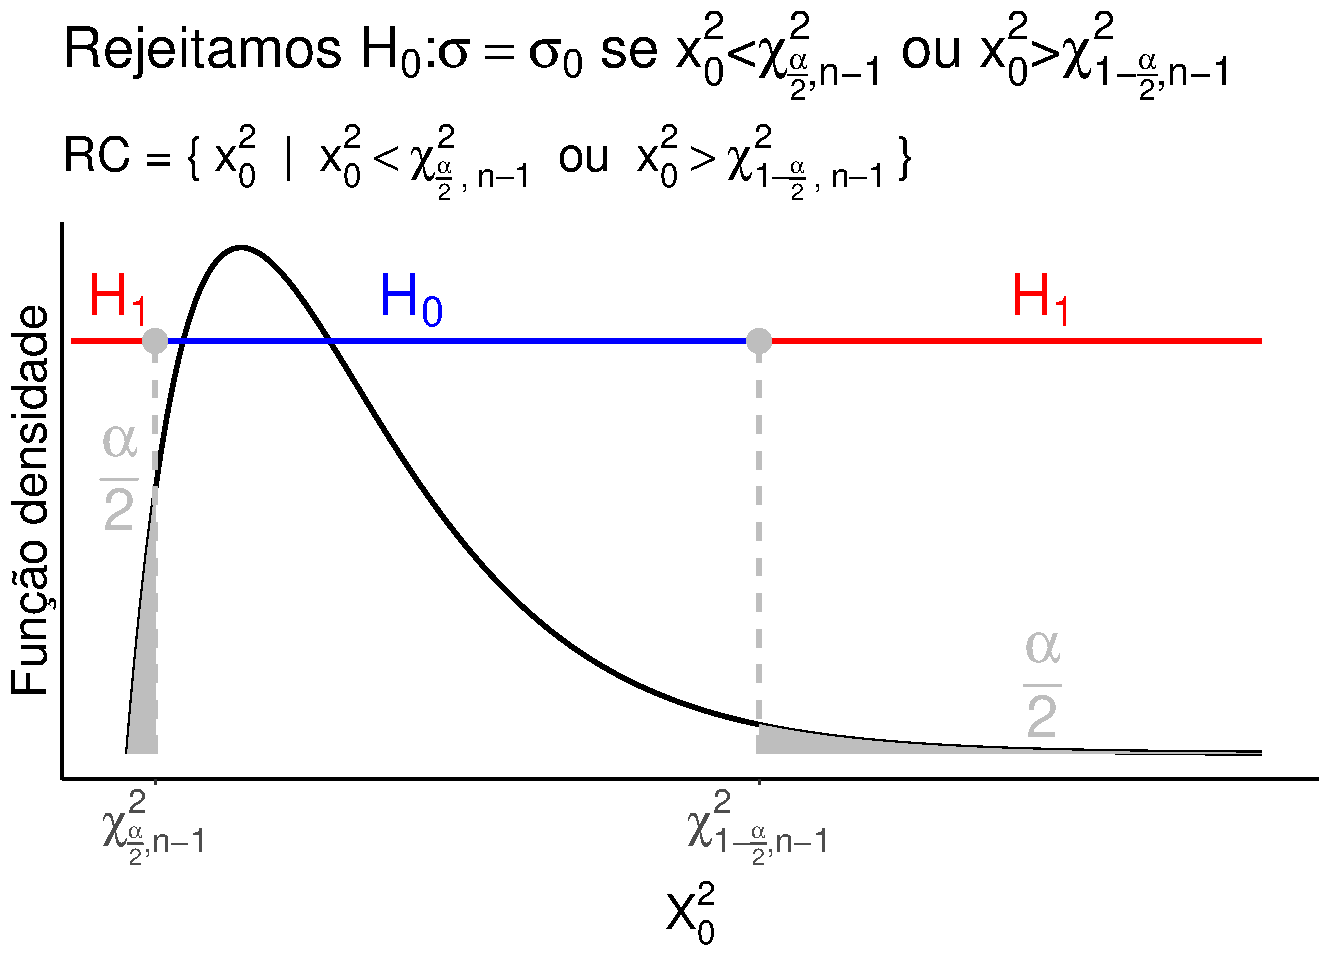
\includegraphics[width=0.315\linewidth]{figures/bilateral-normal-sd-test.pdf} \label{fig:bilateral-normal-sd-test}} \hfill
	\subfloat[][Teste unilateral.]{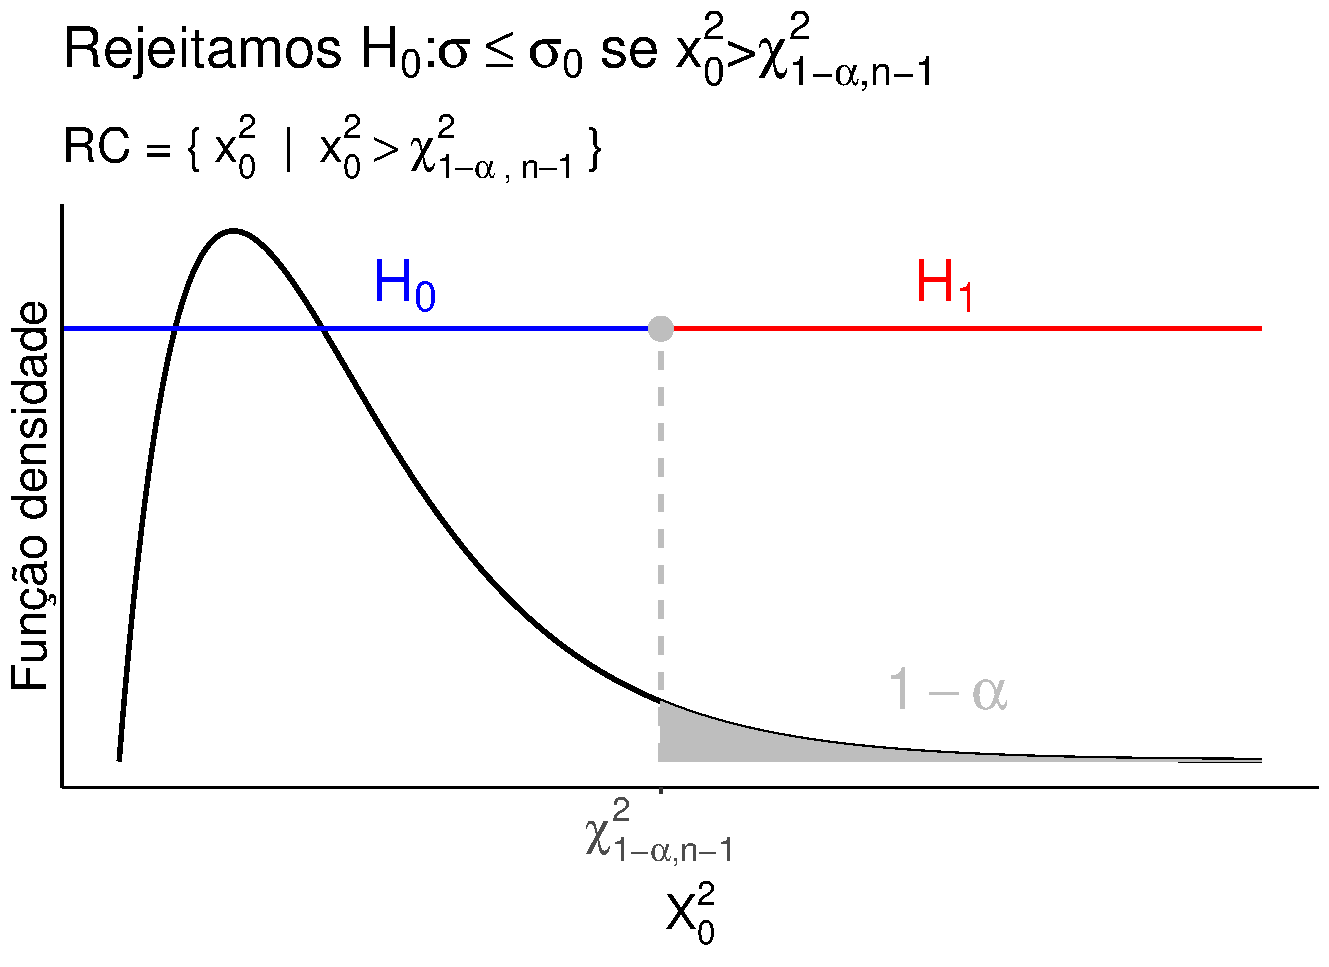
\includegraphics[width=0.315\linewidth]{figures/unilateral-normal-sd-test-h0-lower.pdf} \label{fig:unilateral-normal-sd-test-h0-lower}} \hfill
	\subfloat[][Teste unilateral.]{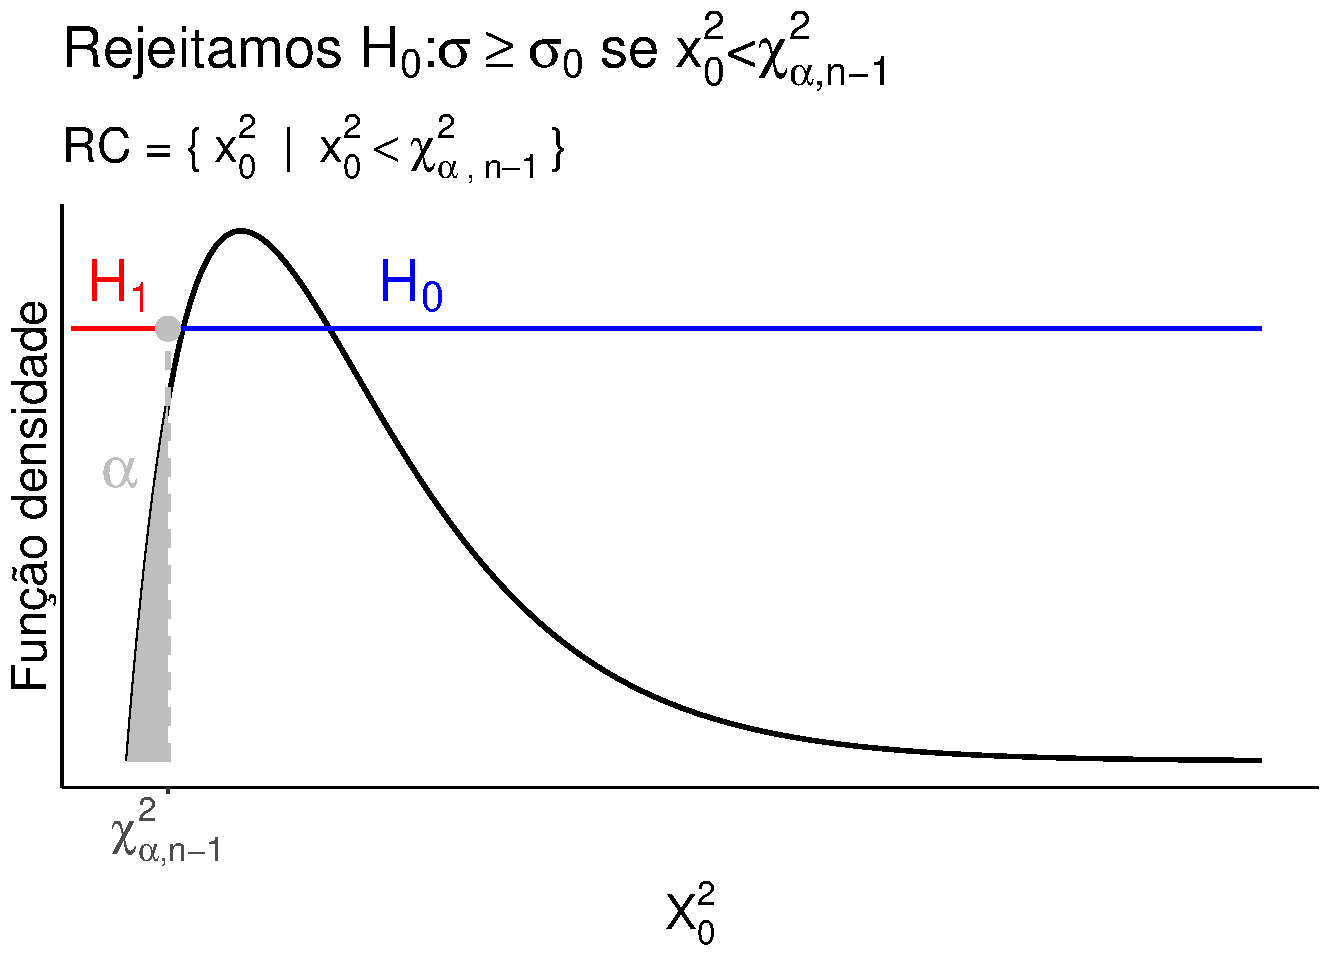
\includegraphics[width=0.315\linewidth]{figures/unilateral-normal-sd-test-h0-upper.pdf} \label{fig:unilateral-normal-sd-test-h0-upper}}		\caption{ Região crítica para o teste de variância.}
\end{figure}


%Chamamos $z_\alpha$, $z_{1-\alpha}$, $z_\frac{\alpha}{2}$ e $z_{1-\frac{\alpha}{2}}$ são chamados de valores críticos.

\normalsize

\end{frame}

\begin{frame}{Distribuição normal: teste da variância.}


\begin{itemize}
	\item Na Figura~\ref{fig:bilateral-normal-sd-test}, testamos $H_0: \sigma = \sigma_0$ versus $H_1: \sigma \neq \sigma_0$. Rejeitamos $H_0$ se $x_0^2 = \frac{(n-1)s^2}{\sigma^2} \in \allowbreak RC=\{x_0^2 \mid x_0^2 < \chi_{\frac{\alpha}{2}; n-1}^2 \mbox{ ou } x_0^2 > \chi_{1-\frac{\alpha}{2};n-1}^2 \}$, em que $P\left(\chi_{n-1}^2 \leq \chi_{\frac{\alpha}{2}, n-1}^2 \right) = \frac{\alpha}{2}$ e $P\left(\chi_{n-1}^2 \leq  \chi_{1-\frac{\alpha}{2};n-1}^2 \right) = 1- \frac{\alpha}{2}$;
	\vfill
	
	\item Na Figura~\ref{fig:unilateral-normal-sd-test-h0-lower}, testamos $H_0: \sigma \leq \sigma_0$ versus $H_1: \sigma > \sigma_0$. Rejeitamos $H_0$ se $x_0^2 = \frac{s^2(n-1)}{\sigma_0^2} \in \allowbreak RC=\{x_0^2 \mid x_0^2 > \chi_{1-\alpha;n-1}^2  \}$, em que $P\left(\chi_{n-1}^2 \leq  \chi_{1-\alpha, n-1} \right) =1- \alpha$;
	\vfill
	
	\item Na Figura~\ref{fig:unilateral-normal-sd-test-h0-upper}, testamos $H_0: \sigma \geq \sigma_0$ versus $H_1: \sigma < \sigma_0$. Rejeitamos $H_0$ se $x_0^2 = \frac{s^2(n-1)}{\sigma_0^2} \in \allowbreak RC=\{x_0^2 \mid x_0^2 < \chi_{\alpha;n-1}^2  \}$, em que $P\left(\chi_{n-1}^2 \leq  \chi_{\alpha;n-1}^2 \right) = \alpha$.
\end{itemize}
Chamamos $\chi_{\alpha; n-1}$, $\chi_{1-\alpha; n-1}$, $\chi_{\frac{\alpha}{2};n-1}$  e $\chi_{1-\frac{\alpha}{2};n-1}$ de valores críticos.
\end{frame}

\begin{frame}{Distribuição normal: teste da variância.}

\large
\begin{block}{Exemplo}
	Uma máquina é usada para encher garrafas com álcool gel. Em uma amostra com $n=20$ garrafas obtemos $s^2=0,0117ml^2$. Se a variância for maior que $0,01$, a proporção de garrafas fora da especificação é inaceitável (pouco ou muito álcool gel), e se a variância for menor que $0,01$, o desgaste da máquina é grande e desnecessária. A máquina está regulamente corretamente ao nível de significância $\alpha=5\%$?
\end{block}
\normalsize

\end{frame}

\begin{frame}{Distribuição normal: teste da variância.}

\begin{block}{Solução}
	\textbf{Passo 1)} Pelo enunciado, temos que testar as hipóteses: $H_0: \sigma = \sigma_0$ e $H_1: \sigma \neq \sigma_0$, em que $\sigma_0=0,01$.

	\textbf{Passo 2)} Nível de significância: $\alpha=5\%$.
	
	\textbf{Passo 3)} Rejeitamos $H_0$ se $ x_0^2  $ for grande ou pequeno. Ou seja, rejeitamos $H_0$ se $ x_0^2  < \chi_{\frac{\alpha}{2};n-1}^2$  e $x_0^2 > \chi_{1-\frac{\alpha}{2}; n-1}^2$. Então, $RC=\{ x_0^2 \mid x_0^2 < \chi_{\frac{\alpha}{2};n-1}^2 \mbox{ ou } x_0^2 > \chi_{1-\frac{\alpha}{2};n-1}^2 \}.$ 

	
	\textbf{Passo 4)} Vamos encontrar o valor crítico da região crítica:
	\begin{itemize}
		\item $P\left( \chi_{n-1}^2 \leq \chi_{\frac{\alpha}{2};n-1}^2 \right) = P\left( \chi_{19}^2  \leq \chi_{0,025;19}^2 \right) = \frac{\alpha}{2} = 0,025$, então $\chi_{0,025;19}^2=8,9065165$;
		\item $P\left( \chi_{n-1}^2 \leq \chi_{\frac{1-\alpha}{2};n-1}^2 \right) = P\left( \chi_{19}^2  \leq \chi_{0,975;19}^2 \right) = 1 - \frac{\alpha}{2} = 0,975$, então $\chi_{0,025;19}^2=32,8523269$.
	\end{itemize}

	\textbf{Passo 5)} Como $x_0^2 = \frac{s^2(n-1)}{\sigma_0^2} = \frac{0,0117\cdot 19}{0,01}=22,23 \not\in RC$, concluímos que não podemos rejeitar $H_0$.
	
	Ou seja, ao nível de significância $\alpha=5\%$, então a variância populacional é aproximadamente $0,01 ml^2$.
\end{block}
\end{frame}

\begin{frame}{Distribuição normal: teste da variância.}

\begin{block}{Solução (valor-p)}
	\begin{figure}[htbp]
		\centering
		\subfloat[][{\scriptsize $x_0^2$ small.}]{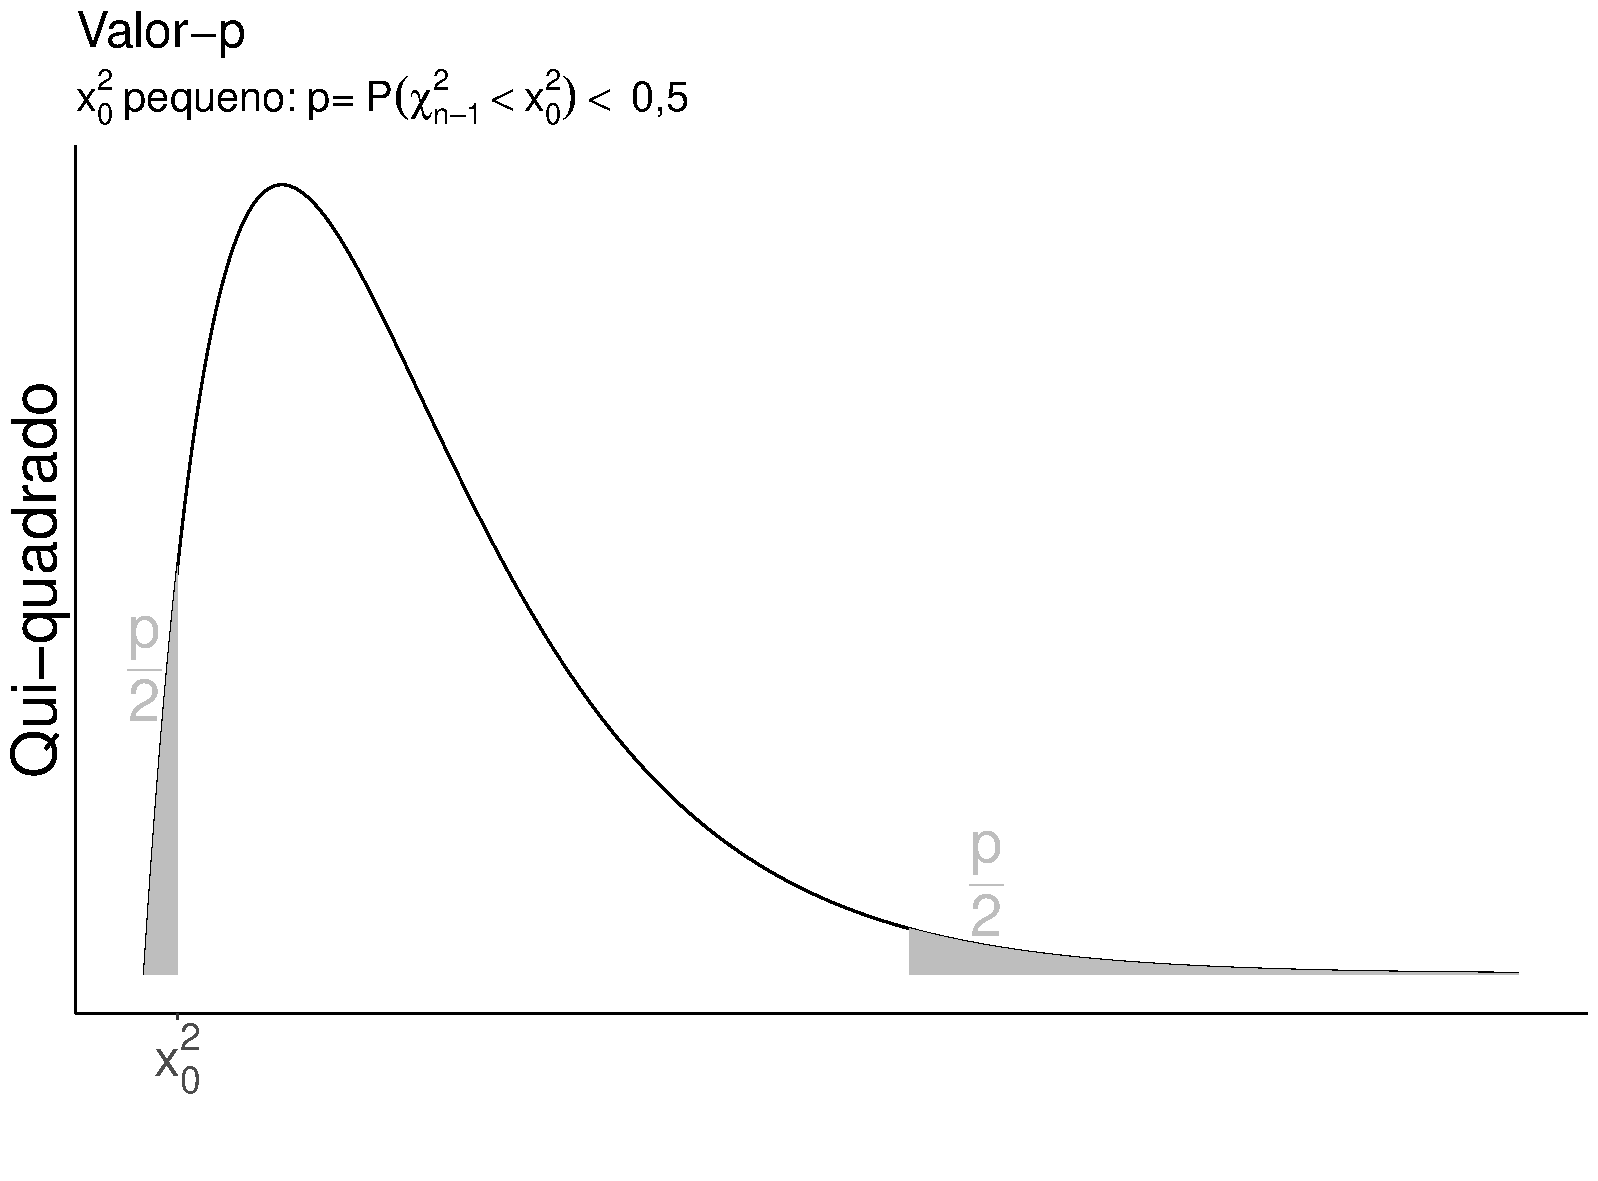
\includegraphics[width=0.45\linewidth]{figures/bilateral-x02-small.pdf} \label{fig:bilateral-x02-smal}}
		\subfloat[][{\scriptsize $x_0^2$ small.}]{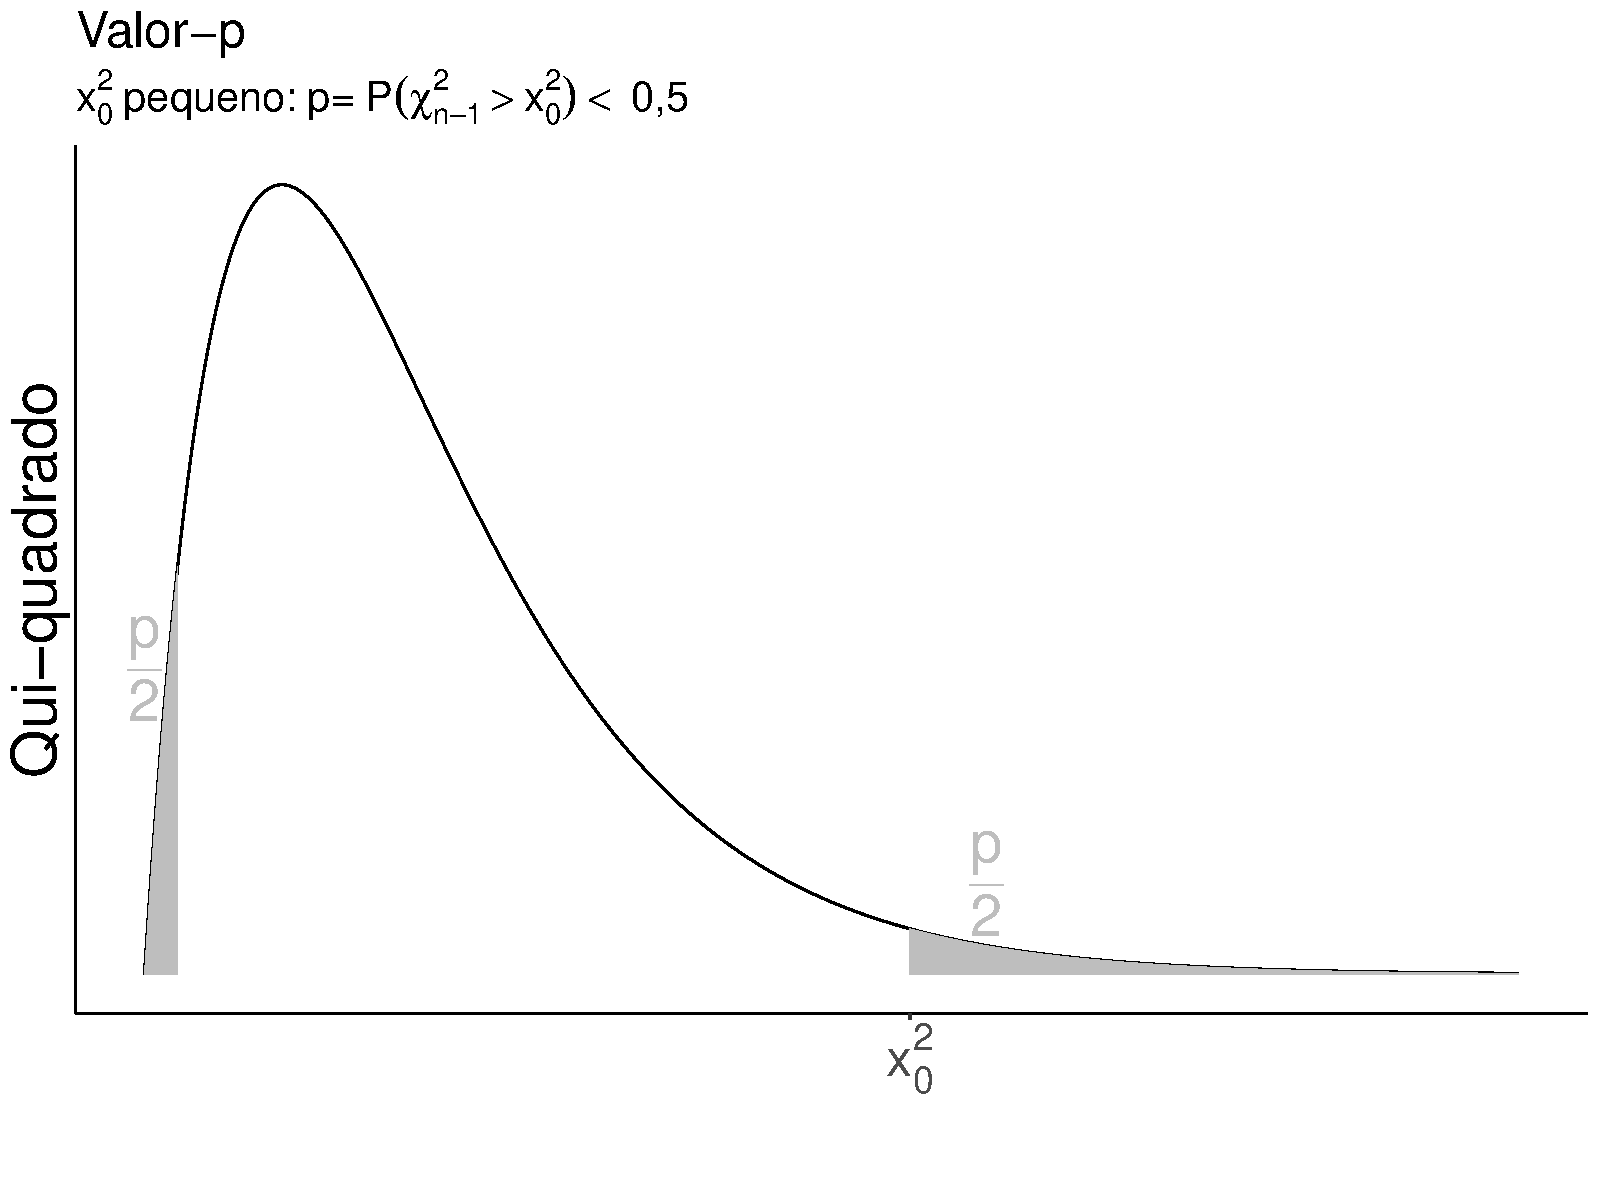
\includegraphics[width=0.45\linewidth]{figures/bilateral-x02-big.pdf} \label{fig:bilateral-x02-big}}
		\caption{Valor-p depende se $P\left( \chi_{n-1}^2 < x_0^2 \right)< 0,5$ ou se $P\left( \chi_{n-1}^2 > x_0^2 \right) < 0,5$.}
	\end{figure}
	
\end{block}

\end{frame}

\begin{frame}{Distribuição normal: teste da variância.}

\begin{block}{Solução (valor-p)}
	O valor-p é calculado através da equação:
	\begin{align*}
	p &= 2 \cdot \min \left(P\left( \chi_{n-1}^2 < x_0^2 \right); P\left( \chi_{n-1}^2 > x_0^2 \right)  \right).
	\end{align*}
\end{block}
\vfill

Como $x_0^2 = \frac{s^2(n-1)}{\sigma_0} = 22,23$ e $ x_0^2  = 22,23$. Note que
\begin{itemize}
	\item $P\left( \chi_{n-1}^2 < x_0^2 \right) = 0,7270$;
	\item $P\left( \chi_{n-1}^2 > x_0^2 \right) = 1 - P\left( \chi_{n-1}^2 < x_0^2 \right) = 0,2730$.
\end{itemize}
Então
\begin{align*}
	p &= 2 \cdot \min \left(P\left( \chi_{n-1}^2 < x_0^2 \right); P\left( \chi_{n-1}^2 > x_0^2 \right)  \right)=  2 \cdot \min\left(0,7270; 0,2730  \right),\\
	&= 2 \cdot 0,2730 =  0,546.
\end{align*}
\vfill

Como $p=0,546 > \alpha=0,05$, ao nível de significância, a variância é aproximadamente $0,01$.
\end{frame}

\begin{frame}{Distribuição normal: teste da variância.}
	
\large	
\begin{block}{Exemplo}
		Uma indústria precisa comprar uma peça em formato cilíndrico e, para cumprir as especificações do INMETRO, o desvio padrão desse diâmetro deve ser, no máximo, $0,5cm$. Um fornecedor do sudeste asiático promete um preço competitivo e afirma que cumpre as especificações do INMETRO. Esta indústria coletou $n=16$ amostras disponíveis no mercado desta peça e obteve um desvio padrão $s=0,646cm$. Ao nível de significância $\alpha=5\%$, você acha que a indústria pode (ou deveria) contratar este fornecedor do sudeste asiático?
	\end{block}
	\vfill
\normalsize
\end{frame}

\begin{frame}{Distribuição normal: teste da variância.}

	\begin{block}{Solução}
	\textbf{Passo 1)} Queremos testar as hipóteses: $H_0: \sigma \leq 0,5$ e $H_1: \sigma > 0,5$;
	
	\textbf{Passo 2)} Nível de significância: $\alpha=5\%$;
	
	\textbf{Passo 3)} Rejeitamos $H_0$ se $X_0^2=\frac{s^2(n-1)}{\sigma_0^2}$ for grande. Ou seja, a região crítica é $RC=\{ x_0^2 \mid x_0^2 > \chi_{1-\alpha; n-1}^2 \}$.
	
	\textbf{Passo 4)} O valor crítico é dado por 
	\begin{itemize}
		\item $P\left( \chi_{n-1}^2 \leq \chi_{1\alpha;n-1}^2 \right) = P\left( \chi_{15}^2 \leq \chi_{0,95;15}^2 \right) =1- \alpha=0,95$, então $\chi_{0,95;15}^2=24,57901$.
	\end{itemize}
	
	\textbf{Passo 5)} Como $s=0,646$ e $x_0=\frac{s^2(n-1)}{\sigma_0^2}=25,04$, rejeitamos $H_0$ ao nível de significância $\alpha=5\%$.
	
	Ou seja, ao nível de significância $\alpha=5\%$, o fornecedor do sudeste asiático não cumpre as especificações do INMETRO e esta indústria não deveria contratar este fornecedor.
\end{block}

\end{frame}

\begin{frame}{Distribuição normal: teste da variância.}

\begin{block}{Solução (valor-p)}
	O valor-p é dado por
	\begin{align*}
		p = P\left( X_0^2 \geq x_0^2 \mid H_0 \right)=1-P\left( \chi_{n-1}^2 \leq x_0^2 \right).
	\end{align*}
\end{block}
\vfill

Como $s=0,646$ e $x_0^2 = \frac{s^2(n-1)}{\sigma_0^2} = \frac{0,0646^2\cdot  15}{0,5^2} = 25,04$, então 
\begin{align*}
p =1- P\left( \chi_{n-1}^2 \leq x_0^2 \right) =1- P\left( \chi_{15}^2 \leq 25,04 \right) = 1-0,951=0,049.
\end{align*}
\vfill

Então, como $p=0,049 < \alpha=0,05$, ao nível de significância $\alpha=5\%$, rejeitamos $H_0$ e não é aconselhável contratar o fornecedor do sudeste asiático.

\end{frame}

\begin{frame}{Distribuição normal: teste de variância.}

\large

\begin{block}{Exemplo}
	Imagine que um pesquisador coletou uma amostra com 16 observações de uma variável aleatória contínua com distribuição normal. Na Tabela~\ref{tab:var-test-unilateral}, apresentamos algumas sobre as hipóteses $H_0: \sigma \geq 1$ e $H_1: \sigma < 1$. Você rejeitaria $H_0$ ao nível de significância $\alpha=5\%$?
	\begin{table}[ht]
		\centering
		\scalebox{0.7}{
		\begin{tabular}{c|c|c|c|c|c|c}
			\toprule[0.05cm]
			tamanho da amostra & $s^2$ & $x_0^2$ & valor-p & Decisão & $\chi_{1-\alpha;n-1}^2$ & $\alpha$ \\ 
			\midrule
			16 & 1,738 &  &  &  &  & $5\%$ \\ 
			\bottomrule[0.05cm]
		\end{tabular}
		}
		\caption{Algumas informações do experimento.} 
		\label{tab:var-test-unilateral}
	\end{table}
\end{block}
\vfill

\normalsize
\end{frame}

\begin{frame}{Distribuição normal: teste de variância.}

\begin{block}{Solução}
	\textbf{Passo 1)} Pelo enunciado, temos as seguintes hipóteses: $H_0: \sigma \geq 1$ e $H_1: \sigma < 1$.
	
	\textbf{Passo 2)} Nível de significância $\alpha=5\%$.
	
	\textbf{Passo 3)} Rejeitamos $H_0$ se $x_0^2=\frac{s^2(n-1)}{\sigma_0^2}$ for grande. Ou seja, a região crítica é $RC=\{ x_0^2 \mid x_0^2 < \chi_{\alpha; n-1}^2 \}$.
	
	\textbf{Passo 4)} Vamos encontrar o valor crítico dado por
	\begin{itemize}
		\item $P\left( \chi_{n-1}^2 \leq \chi_{\alpha;n-1}^2 \right) = P\left( \chi_{n-1}^2 \leq \chi_{0,05;15}^2 \right) = \alpha=0,05$, então $\chi_{0,05;15}^2=7,2609439$.
	\end{itemize}
	
	\textbf{Passo 5)} Como $s^2 = 1,738$ e $x_0^2=\frac{s^2(n-1)}{\sigma_0^2} = 26,07$, como $x_0^2 \not\in RC$ não rejeitamos $H_0$.
	
	Ou seja, ao nível de significância $\alpha=5\%$, não rejeitamos $H_0$.
\end{block}

\end{frame}

\begin{frame}{Distribuição normal: teste de variância.}

\Large

\begin{block}{Solução (valor-p)}
	O valor-p é dado por 
	$$p=P\left( X_0^2 \leq x_0^2 \mid H_0 \right) = P\left( \chi_{n-1}^2 \leq x_0^2  \right).$$
	
	Como $s^2=1,738$ e $x_0^2= \frac{s^2(n-1)}{\sigma_0^2} = 26,07$, então
	\begin{align*}
		p = P\left( \chi_{n-1}^2 \leq 26,07 \right) = 0,9627.
	\end{align*}
	
	Então, como $p=0,9627 > 0,05 = \alpha$, ao nível de significância $\alpha=5\%$, não rejeitamos $H_0$. 
\end{block}

\normalsize

\end{frame}

\subsection{Poder e tamanho da amostra.}

\begin{frame}{Poder do teste: $H_0: \sigma = \sigma_0$ e $H_1: \sigma \neq \sigma_0$.}

\scriptsize

Imagine que
\begin{itemize}
	\item Hipóteses: $H_0: \sigma=\sigma_0$ e $H_1: \sigma \neq \sigma_0$;
	\item $H_1$ é verdade e $\sigma_1 = \sigma_0 + \delta$, em que $\delta \neq 0$;
	\item $x_0^2 = \frac{s^2(n-1)}{\sigma^2} \sim \chi_{n-1}^2$;
	\item Ao nível de significância $\alpha$, temos $RC=\left\{ x_0^2 \mid x_0^2 < \chi_{\frac{\alpha}{2};n-1}^2 \mbox{ ou } \chi_{1-\frac{\alpha}{2};n-1}^2 < x_0^2  \right\}$
\end{itemize}
\vfill

Poder do teste é dado
\begin{align*}
	1-\beta &= 1- P\left( \chi_{\frac{\alpha}{2};n-1}^2 < \frac{s^2(n-1)}{\sigma_0} < \chi_{1-\frac{\alpha}{2};n-1}^2 \mid \sigma^2 = \sigma_1^2  \right)\\
	&=1- P \left( \chi_{\frac{\alpha}{2};n-1}^2 \frac{\sigma_0^2}{\sigma_1^2} < \frac{s^2(n-1)}{\sigma_1} < \chi_{1-\frac{\alpha}{2};n-1}^2 \frac{\sigma_0^2}{\sigma_1^2} \mid \sigma^2 = \sigma_1^2  \right)\\
	&=1- P \left( \chi_{\frac{\alpha}{2};n-1}^2 \frac{\sigma_0^2}{\sigma_1^2} < \chi_{n-1}^2 < \chi_{1-\frac{\alpha}{2};n-1}^2 \frac{\sigma_0^2}{\sigma_1^2} \right)\\
	&=1- P \left( \chi_{n-1}^2 < \chi_{1-\frac{\alpha}{2};n-1}^2 \frac{\sigma_0^2}{\sigma_1^2} \right) + P \left( \chi_{n-1}^2 < \chi_{\frac{\alpha}{2};n-1}^2 \frac{\sigma_0^2}{\sigma_1^2} \right)
\end{align*}
\vfill

A \textcolor{important}{Função Poder}, dado o tamanho da amostra $n$, é uma função das médias populacionais na hipótese alternativa $\pi: (0,\infty) -\{\sigma_0\} \longleftrightarrow [0,1]$ dada por
\begin{align*}
	\pi(\sigma) = 1- P \left( \chi_{n-1}^2 < \chi_{1-\frac{\alpha}{2};n-1}^2 \frac{\sigma_0^2}{\sigma_1^2} \right) + P \left( \chi_{n-1}^2 < \chi_{\frac{\alpha}{2};n-1}^2 \frac{\sigma_0^2}{\sigma_1^2} \right), \qquad \sigma \in  (0,\infty) -\{\sigma_0\}.
\end{align*}
Alguns livros chamam a Função Poder de \textcolor{important}{Curva de Característica Operacional.}
\end{frame}


\begin{frame}{Tamanho da amostra: $H_0: \sigma = \sigma_0$ e $H_1: \sigma \neq \sigma_0$.}

Imagine que
\begin{itemize}
	\item Hipóteses: $H_0: \sigma=\sigma_0$ e $H_1: \sigma \neq \sigma_0$;
	\item $H_1$ é verdade e $\sigma_1 = \sigma_0 + \delta$, em que $\delta \neq 0$;
	\item $x_0^2 = \frac{s^2(n-1)}{\sigma^2} \sim \chi_{n-1}^2$;
	\item Ao nível de significância, temos $RC=\left\{ x_0^2 \mid x_0^2 < \chi_{\frac{\alpha}{2};n-1}^2 \mbox{ ou } \chi_{1-\frac{\alpha}{2};n-1}^2 < x_0^2  \right\}$
\end{itemize}
\vfill

Dado o poder do teste $1-\beta$ (e o erro $\beta$), nível de significância $\alpha$, então encontramos o tamanho da amostra resolvendo a seguinte equação:
\begin{align}\label{eq:sample-size-bilateral-test-s2}
	1-\beta = 1- P \left( \chi_{n-1}^2 < \chi_{1-\frac{\alpha}{2};n-1}^2 \frac{\sigma_0^2}{\sigma_1^2} \right) + P \left( \chi_{n-1}^2 < \chi_{\frac{\alpha}{2};n-1}^2 \frac{\sigma_0^2}{\sigma_1^2} \right).
\end{align}
A equação~\eqref{eq:sample-size-bilateral-test-s2} é resolvida usando métodos numéricos. Tais métodos são estão implementados em diversos \textit{softwares}:
\begin{description}
	\item[No R] \lstinline|pwr_sigma_1pop|
\end{description}

Esta função está no pacote \lstinline|power|, que pode ser instalado usando o pacote \lstinline|devtools|: \lstinline|devtools::install_github("gilberto-sassi/power")|.
\end{frame}

\begin{frame}{Poder do teste: $H_0: \sigma = \sigma_0$ e $H_1: \sigma \neq \sigma_0$.}

\large

\begin{block}{Exemplo}
	Uma máquina é usada para encher garrafas com álcool gel. Considere amostra com $n=20$ garrafas. Se a variância for maior que $0,01$, a proporção de garrafas fora da especificação é inaceitável (pouco ou muito álcool gel), e se a variância for menor que $0,01$, o desgaste da máquina é grande e desnecessária. Se a variância populacional é $\sigma^2=0.02$, qual o poder do teste ao nível de significância $\alpha=5\%$?
\end{block}

\normalsize
\end{frame}

\begin{frame}[fragile]{Poder do teste: $H_0: \sigma = \sigma_0$ e $H_1: \sigma \neq \sigma_0$.}


\begin{block}{Solução}
	\textbf{Passo 1)} Temos as seguintes hipóteses: $H_0: \sigma^2 = 0,01$ e $H_1: \sigma^2 \neq 0,01$;
	
	\textbf{Passo 2)} Nível de significância $\alpha=5\%$;
	
	Primeiro vamos encontrar os valores críticos da distribuição qui-quadrado:
	\begin{itemize}
		\item $P\left( \chi_{n-1}^2 \leq \chi_{\frac{\alpha}{2}; n-1}^2 \right) = P \left( \chi_{19}^2 \leq \chi_{0,025; 19}^2 \right) = \frac{\alpha}{2} = 0,025$, então $\chi_{0,025; 19}^2 = 8,9065165$;
		\item $P\left( \chi_{n-1}^2 \leq \chi_{1-\frac{\alpha}{2}; n-1}^2 \right) = P \left( \chi_{19}^2 \leq \chi_{0,975; 19}^2 \right) = 1-\frac{\alpha}{2} = 0,975$, então $\chi_{0,975; 19}^2 = 32,8523269$.
	\end{itemize}
	
	Como $\sigma_1^2 = 0,01$, então o poder do teste é dado por:
	\begin{align*}
	1-\beta &= 1 -P \left( \chi_{n-1}^2 \leq \chi_{1-\frac{\alpha}{2};n-1} \frac{\sigma_0^2}{\sigma_1^2} \right) + P \left( \chi_{n-1}^2 \leq \chi_{\frac{\alpha}{2};n-1} \frac{\sigma_0^2}{\sigma_1^2} \right)\\
	&=1 -P \left( \chi_{19}^2 \leq 32,8523269 \frac{0,01}{0,02} \right) + P \left( \chi_{n-1}^2 \leq 8,9065165 \frac{0,01}{0,02} \right) = 0,6289.
	\end{align*}
\end{block}

\begin{lstlisting}[language = C, caption = Código no R.]
pwr_sigma_1pop(sigma = sqrt(0.02), sigma0 = sqrt(0.01), n = 20, pwr = NULL,
	alternative = "two.sided", sig_level = 0.05)
\end{lstlisting}

\end{frame}

\begin{frame}{Tamanho da amostra: $H_0: \sigma = \sigma_0$ e $H_1: \sigma \neq \sigma_0$.}

\large
\begin{block}{Exemplo}
	Uma máquina é usada para encher garrafas com álcool gel. Em uma amostra com $n=20$ garrafas. Se a variância for maior que $0,01$, a proporção de garrafas fora da especificação é inaceitável (pouco ou muito álcool gel), e se a variância for menor que $0,01$, o desgaste da máquina é grande e desnecessária. Se a variância populacional é $\sigma^2=0.02$, quantas observações o pesquisador precisa coletar para ter um poder de $99\%$ ao nível de significância $\alpha=5\%$?
\end{block}
\normalsize

\end{frame}

\begin{frame}[fragile]{Tamanho da amostra: $H_0: \sigma = \sigma_0$ e $H_1: \sigma \neq \sigma_0$.}

\large

\begin{block}{solução}
	\textbf{Passo 1)} Temos que testar as hipóteses: $H_0: \sigma = 0,01$ e $H_1: \sigma \neq 0,01$;
	
	\textbf{Passo 2)} Nível de significância $\alpha=0,05$;
	
	Como o poder do teste é $1-\beta=99\%$, o nível de significância é $\alpha=5\%$, e variância populacional é $\sigma_1^2=0,02$, então o tamanho amostral é solução em $n$ da seguinte equação:
	$$1- \beta = 0,99 = 1 - P\left( \chi_{n-1}^2 \leq \chi_{1-\frac{\alpha}{2};n-1}^2 \frac{\sigma_0^2}{\sigma_1^2} \right) + P \left( \chi_{n-1}^2 \leq \chi_{\frac{\alpha}{2};n-1}^2 \frac{\sigma_0^2}{\sigma_1^2} \right).$$
\end{block}

Precisamos coletar $n=81$ frascos.

\begin{lstlisting}[language = C, caption = Código no R.]
pwr_sigma_1pop(sigma = sqrt(0.02), sigma0 = sqrt(0.01), n = NULL, pwr = 0.99,
		alternative = "two.sided", sig_level = 0.05)
\end{lstlisting}

\normalsize

\end{frame}

\begin{frame}{Poder do teste: $H_0: \sigma \geq \sigma_0$ e $H_1: \sigma < \sigma_0$}

\small

Imagine que
\begin{itemize}
	\item Hipóteses: $H_0: \sigma \geq \sigma_0$ e $H_1: \sigma < \sigma_0$;
	\item $H_1$ é verdade e $\sigma = \sigma_1 < \sigma_0$;
	\item $x_0^2 = \frac{s^2(n-1)}{\sigma_1^2} \sim \chi_{n-1}^2$;
	\item Ao nível de significância $\alpha=5\%$, a região crítica é dada por $RC=\left\{ x_0^2 \mid x_0^2 < \chi_{\alpha; n-1}^2 \right\}$.
\end{itemize}
\vfill

O poder do teste é dado
\begin{align*}
	1- \beta &= 1 - P \left( \frac{s^2(n-1)}{\sigma_0^2} \geq \chi_{\alpha;n-1}^2 \mid \sigma = \sigma_1 \right)= P \left( \frac{s^2(n-1)}{\sigma_1^2} \leq \chi_{\alpha; n-1}^2 \frac{\sigma_0^2}{\sigma_1^2} \mid \sigma = \sigma_1 \right)\\ 
	&= P \left( \chi_{n-1}^2 \leq \chi_{\alpha; n-1}^2 \frac{\sigma_0^2}{\sigma_1^2} \right).
\end{align*}

A \textcolor{important}{Função Poder}, dado o tamanho da amostra $n$, é uma função das médias populacionais na hipótese alternativa: $\pi: (\sigma_0, \infty) \longleftrightarrow [0,1]$ dada por
$$\pi(\sigma) = P \left( \chi_{n-1}^2 \leq \chi_{\alpha; n-1}^2 \frac{\sigma_0^2}{\sigma_1^2} \right), \quad \sigma \in (\sigma_0, \infty).$$
Alguns livros chamam a Função Poder de  \textcolor{important}{Curva de Característica Operacional.}

\normalsize

\end{frame}


\begin{frame}{Tamanho da amostra: $H_0: \sigma \geq \sigma_0$ e $H_1: \sigma < \sigma_0$}

Imagine que
\begin{itemize}
	\item Hipóteses: $H_0: \sigma \geq \sigma_0$ e $H_1: \sigma < \sigma_0$;
	\item $H_1$ é verdade e $\sigma = \sigma_1 < \sigma_0$;
	\item $x_0^2 = \frac{s^2(n-1)}{\sigma_1^2} \sim \chi_{n-1}^2$;
	\item Ao nível de significância $\alpha=5\%$,  $RC=\left\{ x_0^2 \mid x_0^2 < \chi_{\alpha; n-1}^2 \right\}$
\end{itemize}
\vfill

Dado o poder do teste $1-\beta$ (e o erro $\beta$), nível de significância $\alpha$, então encontramos o tamanho da amostra resolvendo a seguinte equação
\begin{align} \label{eq:sample-size-unilateral-test-s2-h0-upper}
	1-\beta = P \left( \chi_{n-1}^2 \leq \chi_{\alpha; n-1}^2 \frac{\sigma_0^2}{\sigma_1^2} \right).
\end{align}

A equação~\eqref{eq:sample-size-unilateral-test-s2-h0-upper} é resolvida usando métodos numéricos. Tais métodos estão implementados em diversos \textit{softwares}:
\begin{description}
	\item[No R] \lstinline|pwr_sigma_1pop|
\end{description}

Esta função está no pacote \lstinline|power|, que pode ser instalado usando o pacote \lstinline|devtools|: \lstinline|devtools::install_github("gilberto-sassi/power")|.
\end{frame}

\begin{frame}{Poder do teste: $H_0: \sigma \geq \sigma_0$ e $H_1: \sigma < \sigma_0$.}

\large

\begin{block}{Exemplo}
	Imagine que um pesquisador coletou uma amostra com 16 observações de uma variável aleatória contínua com distribuição normal. Na Tabela~\ref{tab:var-test-unilateral-h0-lower}, apresentamos algumas sobre as hipóteses $H_0: \sigma \geq 1$ e $H_1: \sigma < 0,5$. Se o desvio padrão populacional é $\sigma_1 = 2$, ao nível de significância $\alpha=5\%$, qual o poder do teste?
	\begin{table}[ht]
		\centering
		\scalebox{0.6}{
		\begin{tabular}{c|c|c|c}
			\toprule[0.05cm]
			tamanho da amostra &  $1-\beta$ & Desvio padrão populacional ($\sigma_1$) & $\alpha$ \\ 
			\midrule
			16 &   & $0,5$ & $5\%$ \\ 
			\bottomrule[0.05cm]
		\end{tabular}
		}
		\caption{Algumas informações do experimento.} 
		\label{tab:var-test-unilateral-h0-lower}
	\end{table}
\end{block}
\normalsize

\end{frame}

\begin{frame}[fragile]{Poder do teste: $H_0: \sigma \geq \sigma_0$ e $H_1: \sigma < \sigma_0$.}
\begin{block}{Solução}
	\textbf{Passo 1)} Pelo enunciado temos os seguintes hipóteses: $H_0: \sigma \geq 1 $ e $H_1: \sigma < 1$;
	
	\textbf{Passo 2)} Nível de significância $\alpha=5\%$;
	
	Note que $\alpha=0,05$, $n=16$, $\sigma_0 = 1$ e $\sigma_1 = 0,5$.
	
	Primeiro vamos encontrar os quantis da distribuição qui-quadrado:
	\begin{itemize}
		\item $P\left(  \chi_{n-1}^2 \leq \chi_{\alpha;n-1}^2 \right) = P\left(  \chi_{15}^2 \leq \chi_{0,05;15}^2 \right) = \alpha=0,05$, então $\chi_{0,05;15}^2 = 7,2609439$.
	\end{itemize}
	
	Então o poder do teste é dado
	$$1-\beta =  P \left( \chi_{n-1}^2 \leq \chi_{0,05;15}^2 \frac{\sigma_0^2}{\sigma_1^2} \right) =  P \left(\chi_{15}^2 \leq 7,2609439 \frac{1}{0,5^2}  \right) = 0,9841.$$
\end{block}

\begin{lstlisting}[language = C, caption = Código no R.]
pwr_sigma_1pop(sigma = 0.5, sigma0 = 1, n = 16, pwr = NULL,
		alternative = "less", sig_level = 0.05)
\end{lstlisting}

\end{frame}


\begin{frame}{Tamanho da amostra: $H_0: \sigma \geq \sigma_0$ e $H_1: \sigma < \sigma_0$.}

\large
\begin{block}{Exemplo}
Imagine que um pesquisador coletou uma amostra com 16 observações de uma variável aleatória contínua com distribuição normal. Na Tabela~\ref{tab:var-test-unilateral-h0-lower-sample-size}, apresentamos algumas sobre as hipóteses $H_0: \sigma \geq 1$ e $H_1: \sigma < 1$. Se o desvio padrão populacional é $\sigma_1 = 0,5$, ao nível de significância $\alpha=5\%$, quantas observações precisam ser coletadas para termos poder de teste $1-\beta=99\%$?
\begin{table}[ht]
	\centering
	\begin{tabular}{c|c|c|c}
		\toprule[0.05cm]
		tamanho da amostra &  $1-\beta$  &  Desvio padrão populacional ($\sigma_1$) & $\alpha$ \\ 
		\midrule
		& $99\%$  & $2$ & $5\%$ \\ 
		\bottomrule[0.05cm]
	\end{tabular}
	\caption{Algumas informações do experimento.} 
	\label{tab:var-test-unilateral-h0-lower-sample-size}
\end{table}
\end{block}
\normalsize
\end{frame}

\begin{frame}[fragile]{Tamanho da amostra: $H_0: \sigma \geq \sigma_0$ e $H_1: \sigma < \sigma_0$.}

\begin{block}{Solução}
	\textbf{Passo 1)} Pelo enunciado temos os seguintes hipóteses: $H_0: \sigma \geq 1 $ e $H_1: \sigma < 1$;
	
	\textbf{Passo 2)} Nível de significância $\alpha=5\%$;
	
	Como o nível de significância $\alpha=5\%$, poder do teste $1-\beta=99\%$, $\sigma_0^2=1$ e $\sigma_1^2=0,5^2$.
	
	Então o tamanho da amostra é solução da seguinte equação:
	$$1-\beta=0,99=1-P\left( \chi_{n-1}^2 \leq \chi_{1-\alpha;n-1}^2 \frac{\sigma_0^2}{\sigma_1^2} \right) = P\left( \chi_{15}^2 \leq \chi_{0,99;n-1}^2 \frac{1^2}{0,5^2} \right).$$
	
	Então, o tamanho \sout{mínimo} da amostra deve ser $n=18$ observações.
\end{block}

\begin{lstlisting}[language = C, caption = Código no R.]
pwr_sigma_1pop(sigma = 0.5, sigma0 = 1, n = NULL, pwr = 0.99,
		alternative = "less", sig_level = 0.05)
\end{lstlisting}

\end{frame}

\begin{frame}{Poder do teste: $H_0: \sigma \leq \sigma_0$ e $H_1: \sigma > \sigma_0$}

Imagine que
\begin{itemize}
	\item Hipóteses: $H_0: \sigma \leq \sigma_0$ e $H_1: \sigma > \sigma_0$;
	\item $H_1$ é verdade e $\sigma = \sigma_1 > \sigma_0$;
	\item $x_0^2 = \frac{s^2(n-1)}{\sigma_1^2} \sim \chi_{n-1}^2$;
	\item Ao nível de significância $\alpha=5\%$, a região crítica é dada por $RC=\left\{ x_0^2 \mid x_0^2 > \chi_{1-\alpha; n-1}^2 \right\}$
\end{itemize}
\vfill

O poder do teste é dado
\begin{align*}
1- \beta &= 1 - P \left( \frac{s^2(n-1)}{\sigma_0^2} \leq \chi_{1-\alpha;n-1}^2 \mid \sigma = \sigma_1 \right)\\
&=1- P \left( \frac{s^2(n-1)}{\sigma_1^2} \leq \chi_{1-\alpha; n-1}^2 \frac{\sigma_0^2}{\sigma_1^2} \mid \sigma = \sigma_1 \right)= 1- P \left( \chi_{n-1}^2 \leq \chi_{1-\alpha; n-1}^2 \frac{\sigma_0^2}{\sigma_1^2} \right).
\end{align*}

A \textcolor{important}{Função Poder}, dado o tamanho da amostra $n$, é uma função das médias populacionais na hipótese alternativa: $\pi: (0,\sigma_0) \longleftrightarrow [0,1]$ dada por
$$\pi(\sigma) = 1 - P \left( \chi_{n-1}^2 \leq \chi_{1-\alpha; n-1}^2 \frac{\sigma_0^2}{\sigma^2} \right), \quad \sigma \in (0,\sigma_0).$$
Alguns livros chamam a Função Poder de  \textcolor{important}{Curva de Característica Operacional.}
\end{frame}


\begin{frame}{Tamanho da amostra: $H_0: \sigma \leq \sigma_0$ e $H_1: \sigma > \sigma_0$}

Imagine que
\begin{itemize}
\item Hipóteses: $H_0: \sigma \leq \sigma_0$ e $H_1: \sigma > \sigma_0$;
\item $H_1$ é verdade e $\sigma = \sigma_1 > \sigma_0$;
\item $x_0^2 = \frac{s^2(n-1)}{\sigma_1^2} \sim \chi_{n-1}^2$;
\item Ao nível de significância $\alpha=5\%$, $RC=\left\{ x_0^2 \mid x_0^2 > \chi_{1-\alpha; n-1}^2 \right\}$
\end{itemize}
\vfill

Dado o poder do teste $1-\beta$ (e o erro $\beta$), nível de significância $\alpha$, então encontramos o tamanho da amostra resolvendo a seguinte equação
\begin{align} \label{eq:sample-size-unilateral-test-s2-h0-lower}
1-\beta =1- P \left( \chi_{n-1}^2 \leq \chi_{1-\alpha; n-1}^2 \frac{\sigma_0^2}{\sigma_1^2} \right).
\end{align}

A equação~\eqref{eq:sample-size-unilateral-test-s2-h0-lower} é resolvida usando métodos numéricos. Tais métodos estão implementados em diversos \textit{softwares}:
\begin{description}
\item[No R] \lstinline|pwr_sigma_1pop|
\end{description}

Esta função está no pacote \lstinline|power|, que pode ser instalado usando o pacote \lstinline|devtools|: \lstinline|devtools::install_github("gilberto-sassi/power")|.
\end{frame}

\begin{frame}{Poder do teste: $H_0: \sigma \leq \sigma_0$ e $H_1: \sigma > \sigma_0$.}

\large

\begin{block}{Exemplo}
	Uma indústria precisa comprar uma peça em formato cilíndrico e, para cumprir as especificações do INMETRO, o desvio padrão desse diâmetro deve ser, no máximo, $0,5cm$. Um fornecedor do sudeste asiático promete um preço competitivo e afirma que cumpre as especificações do INMETRO. Esta indústria coletou $n=16$ amostras disponíveis no mercado desta peça. Se a variância populacional do diâmetro for $\sigma=0,75$. Ao nível de significância $\alpha=5\%$, qual o poder do teste?
\end{block}
\normalsize

\end{frame}

\begin{frame}[fragile]{Poder do teste: $H_0: \sigma \leq \sigma_0$ e $H_1: \sigma > \sigma_0$.}

\begin{block}{Solução}
	\textbf{Passo 1)} Temos as seguintes hipóteses: $H_0: \sigma^2 \leq 0,5^2$ e $H_1: \sigma^2 > 0,5^2$;
	
	\textbf{Passo 2)} Nível de significância $\alpha = 5\%$;
	
	Como o poder do teste $n=16$, o nível de significância $\alpha=5\%$ e a variância populacional é $\sigma_1^2 = 0,75^2$.
	
	Primeiro vamos encontrar os quantis da distribuição qui-quadrado:
	\begin{itemize}
		\item $P\left( \chi_{n-1}^2 \leq \chi_{1-\alpha; n-1}^2 \right) = P\left( \chi_{15}^2 \leq \chi_{0,95; 15}^2 \right) =1- \alpha = 0,95$, então $\chi_{0,95; 15}^2 = 24,9957901$.
	\end{itemize}
	
	Então o poder do teste é dado por
	\begin{align*}
	1-\beta &=1- P\left( \chi_{n-1}^2 \leq \chi_{1-\alpha; n-1}^2\frac{\sigma_0^2}{\sigma_1^2} \right) =1- P \left( \chi_{15}^2 \leq \chi_{1-\alpha; 15}^2\frac{0,5^2}{0,75^2} \right)\\ 
	&=1- P \left( \chi_{15}^2 \leq  24,9957901 \frac{0,5^2}{0,75^2} \right)= 0,7448.
	\end{align*}
\end{block}

\begin{lstlisting}[language = C, caption = Código no R.]
pwr_sigma_1pop(sigma = 0.75, sigma0 = 0.5, n = 16, pwr = NULL,
		alternative = "greater", sig_level = 0.05)
\end{lstlisting}

\end{frame}


\begin{frame}{Tamanho da amostra: $H_0: \sigma \leq \sigma_0$ e $H_1: \sigma > \sigma_0$.}

\large

\begin{block}{Exemplo}
Uma indústria precisa comprar uma peça em formato cilíndrico e, para cumprir as especificações do INMETRO, o desvio padrão desse diâmetro deve ser, no máximo, $0,5cm$. Um fornecedor do sudeste asiático promete um preço competitivo e afirma que cumpre as especificações do INMETRO. Se a variância populacional do diâmetro for $\sigma=0,75$. Ao nível de significância $\alpha=5\%$, quantas peças precisamos analisar para termos um poder de teste de $99\%$?
\end{block}

\normalsize
\end{frame}

\begin{frame}[fragile]{Tamanho da amostra: $H_0: \sigma \leq \sigma_0$ e $H_1: \sigma > \sigma_0$.}

\normalsize
\begin{block}{Solução}
	\textbf{Passo 1)} Temos as seguintes hipóteses: $H_0: \sigma^2 \leq 0,5^2$ e $H_1: \sigma^2 > 0,5^2$;
	
	\textbf{Passo 2)} Nível de significância $\alpha = 5\%$;
	
	Como a variância populacional é $\sigma=0,75$, poder $99\%$, $\sigma=0,75$ e $\sigma_0 = 0,5$.
	
	Então o tamanho da amostra é solução em $n$ da equação abaixo:
	$$1-\beta=0,99 =1- P \left( \chi_{n-1}^2 \leq \chi_{1-\alpha;n-1}^2 \frac{\sigma_0^2}{\sigma_1^2} \right) =1- P \left( \chi_{n-1}^2 \leq \chi_{0,95;n-1}^2 \frac{0,5^2}{0,75^2} \right).$$
	
	Então o tamanho \sout{mínimo} da amostra deve ser $n=53$.
\end{block}

\begin{lstlisting}[language = C, caption = Código no R.]
pwr_sigma_1pop(sigma = 0.75, sigma0 = 0.5, n = NULL, pwr = 0.99,
		alternative = "greater", sig_level = 0.05)
\end{lstlisting}

\normalsize
\end{frame}

\section{Teste para proporção: $p$ ($n \geq 40$).}

\begin{frame}{Teste para proporção.}

\normalsize

Sejam
\begin{itemize}
	\item $x_1, \dots, x_n$ valores amostrados de $Bernoulli(p)$;
	\item $\alpha$ é o nível de significância (estabelecido pelo pesquisador e geralmente $\alpha=5\%$). 
\end{itemize}
\vfill

Queremos testar as seguintes hipóteses:
\begin{itemize}
	\item Teste bilateral: $H_0: p= p_0$ e $H_1: p \neq p_0$;
	\item Teste unilateral: $H_0: p \leq p_0$ e $H_1: p > p_0$;
	\item Teste unilateral: $H_0: p \geq p_0$ e $H_1: p < p_0$.
\end{itemize}
\vfill

\textbf{Ideia:} Primeiro calculamos a distância padronizada de $\hat{p} = \frac{x_1 + \dots + x_n}{n}$ e $p_0$: $z_0=\frac{(\hat{p} - p_0)\sqrt{n}}{\sqrt{p_0 (1-p_0)}}$. Então, 
\begin{itemize}
	\item Teste bilateral: Rejeitamos $H_0: p - p_0 = 0$ se $\lvert z_0 \rvert$ for grande;
	\item Teste unilateral: Rejeitamos $H_0: p - p_0 \leq 0$ se $z_0$ for grande;
	\item Teste unilateral: Rejeitamos $H_0: p - p_o \geq 0$ se $z_0$ for pequeno.
\end{itemize}

\end{frame}


\begin{frame}{Teste para proporção.}

\normalsize

\begin{figure}[htbp]
	\centering
	\subfloat[][Teste bilateral.]{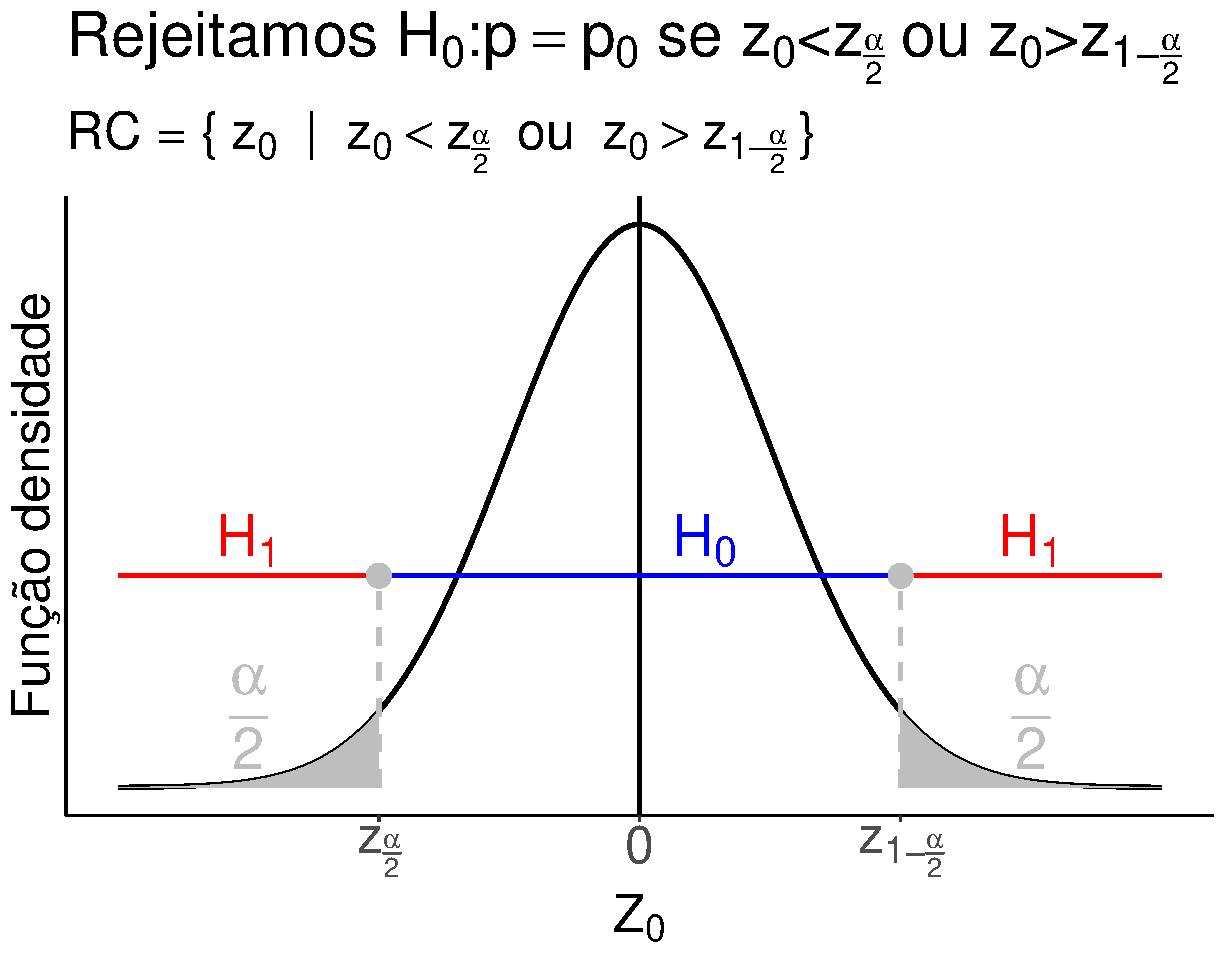
\includegraphics[width=0.32\linewidth]{figures/proportion-bilateral.pdf} \label{fig:proportion-bilateral}} \hfill
	\subfloat[][Teste unilateral.]{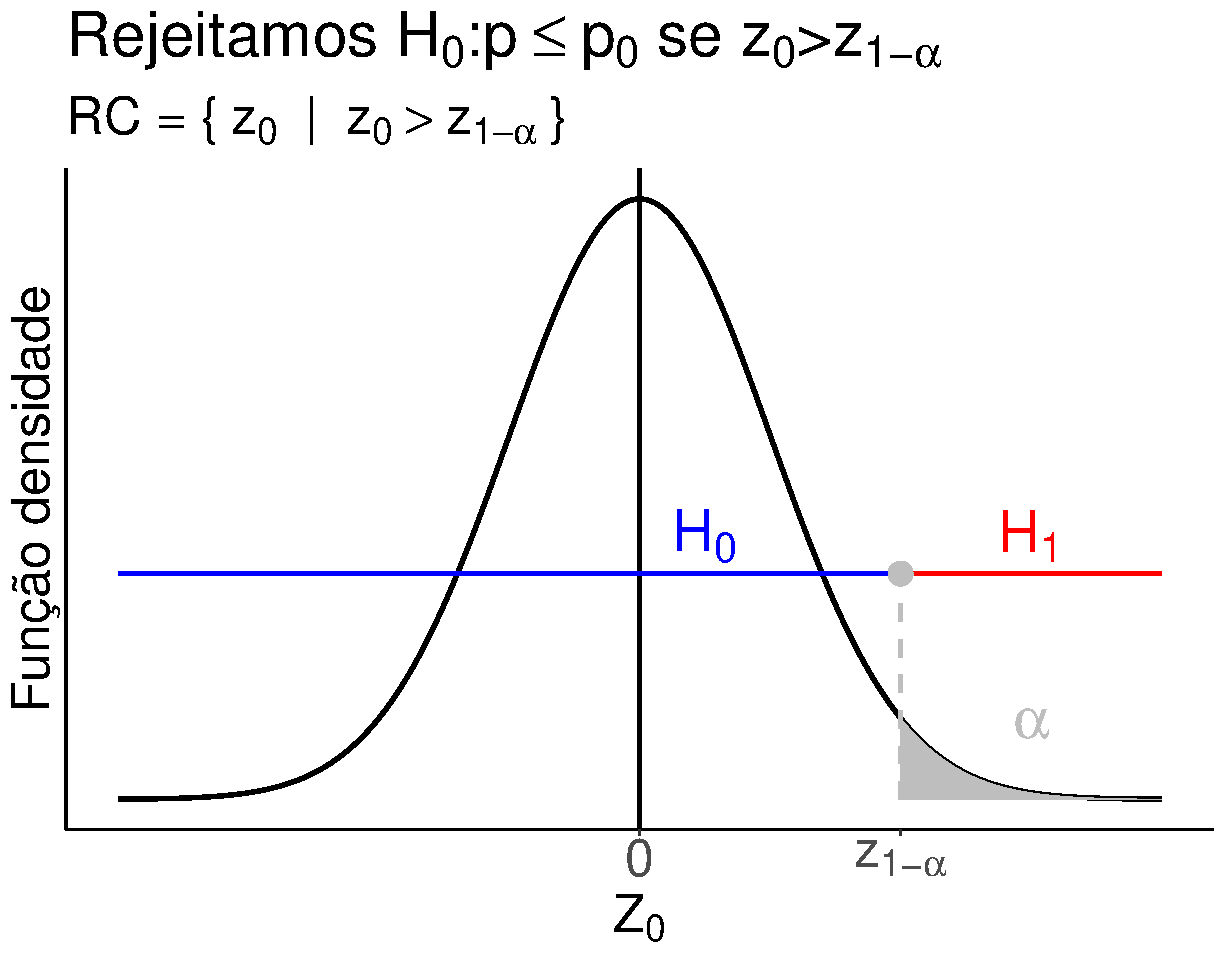
\includegraphics[width=0.32\linewidth]{figures/proportion-h1-upper.pdf} \label{fig:proportion-h1-upper}} \hfill
	\subfloat[][Teste unilateral.]{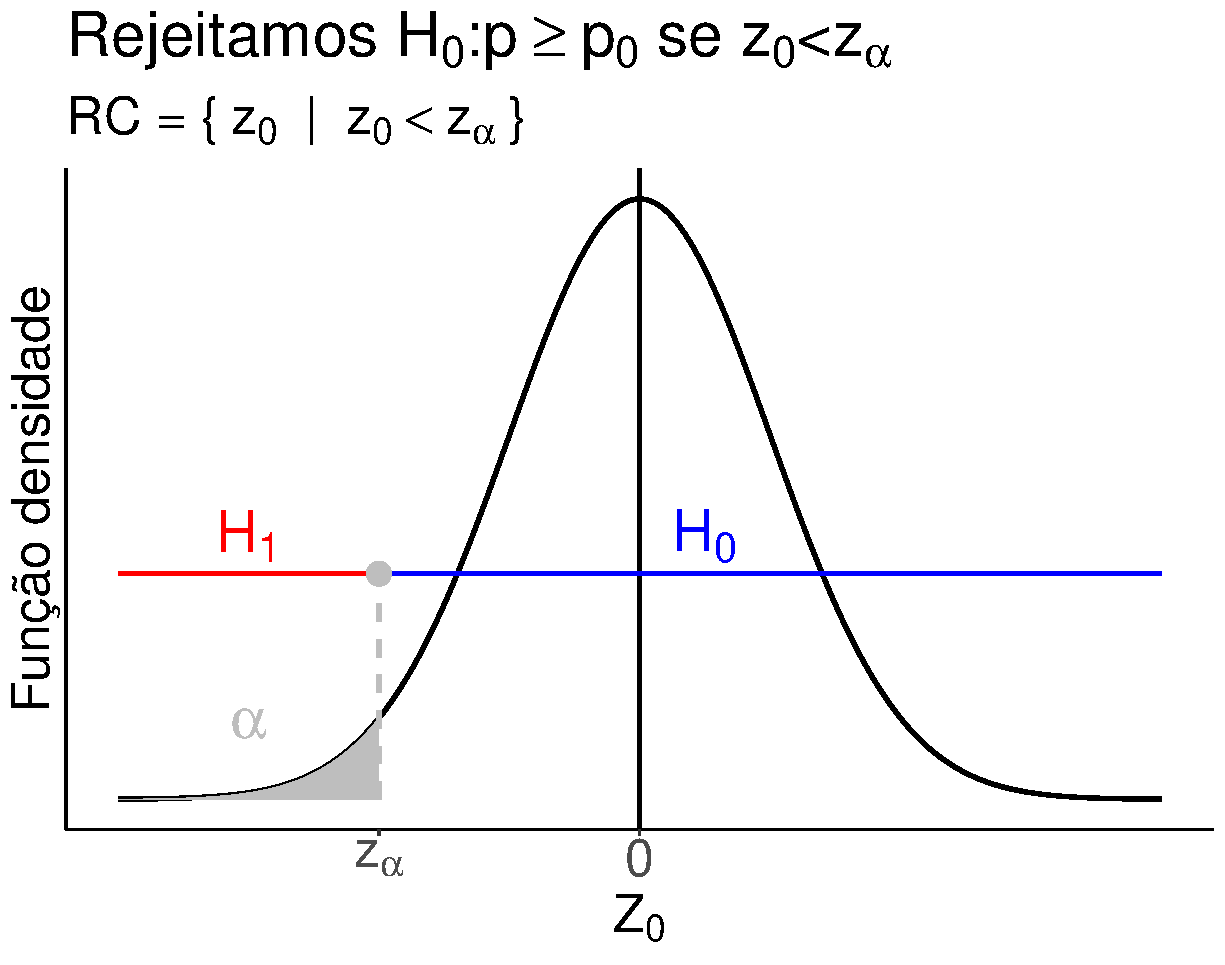
\includegraphics[width=0.32\linewidth]{figures/proportion-h1-lower.pdf} \label{fig:proportion-h1-lower}}
	\caption{Região crítica para o teste Z.}
\end{figure}

\normalsize

\end{frame}

\begin{frame}{Teste para proporção.}

\begin{itemize}
	\item Na Figura~\ref{fig:proportion-bilateral}, testamos $H_0: p = p_0$ versus $H_1: p \neq p_0$. Rejeitamos $H_0$ se $z_0 = \frac{(\hat{p} - p_0)\sqrt{n}}{\sqrt{p_0(1-p_0)}} \in \allowbreak RC=\{z_0 \mid z_0 < z_\frac{\alpha}{2} \mbox{ ou } z_0 > z_{1-\frac{\alpha}{2}} \}$, em que $\Phi\left( z_\frac{\alpha}{2} \right) = \frac{\alpha}{2}$ e $\Phi\left( z_{1-\frac{\alpha}{2}} \right) = 1- \frac{\alpha}{2}$;
	\vfill
	
	\item Na Figura~\ref{fig:proportion-h1-upper}, testamos $H_0: p \leq p_0$ versus $H_1: p > p_0$. Rejeitamos $H_0$ se $z_0 = \frac{(\hat{p} - p_0)\sqrt{n}}{\sqrt{p_0(1-p_0)}} \in \allowbreak RC=\{z_0 \mid z_0 > z_{1-\alpha}  \}$, em que $\Phi\left( z_{1-\alpha} \right) =1- \alpha$;
	\vfill
	
	\item Na Figura~\ref{fig:proportion-h1-lower}, testamos $H_0: p \geq p_0$ versus $H_1: p < p_0$. Rejeitamos $H_0$ se $z_0 = \frac{(\hat{p} - p_0)\sqrt{n}}{\sqrt{p_0(1-p_0)}} \in \allowbreak RC=\{z_0 \mid z_0 < z_{\alpha}  \}$, em que $\Phi\left( z_{\alpha} \right) = \alpha$.
\end{itemize}
Chamamos $z_\alpha$, $z_{1-\alpha}$, $z_\frac{\alpha}{2}$ e $z_{1-\frac{\alpha}{2}}$ são chamados de valores críticos.

\end{frame}


\begin{frame}{Teste para proporção.}

\large

\begin{block}{Exemplo}
	Suponha que uma marca entrevistou $1000$ consumidores, e $850$ afirmaram estarem satisfeitos com a marca. Ao nível de significância $\alpha=5\%$, decida entre as hipóteses $H_0: p = 0,9$ e $H_1: p\neq 0,9$, em que $p$ é a proporção populacional de consumidores satisfeitos com a marca. Calcule o valor-p.
\end{block}

\normalsize

\end{frame}

\begin{frame}{Teste para proporção.}

\begin{block}{Solução}
	\textbf{Passo 1)} Pelo enunciado, queremos testar as seguintes hipóteses: $H_0: p=0,9$ e $H_1:p \neq 0,9$;
	
	\textbf{Passo 2)} Nível de significância $\alpha=5\%$;
	
	\textbf{Passo 3)} Rejeitamos $H_0$ se $\lvert z_0  \rvert = \left\lvert \frac{(\hat{p} - p_0)\sqrt{n}}{\sqrt{p_0(1-p_0)}} \right\rvert$ for grande. Ou seja, $RC=\left\{ z_0 \mid z_{\frac{\alpha}{2}} < z_0 < z_{1-\frac{\alpha}{2}} \right\}$.
	
	\textbf{Passo 4)} Vamos encontrar os valores críticos:
	\begin{itemize}
		\item $\Phi\left( z_\frac{\alpha}{2} \right) = \Phi\left( z_{0,025} \right) = \frac{\alpha}{2} = 0,025$, então $z_{0,025} = -1,96$;
		\item $\Phi\left( z_{1-\frac{\alpha}{2}} \right) = \Phi\left( z_{0,975} \right) =1- \frac{\alpha}{2} = 0,975$, então $z_{0,975} = 1,96$.
	\end{itemize}
	
	\textbf{Passo 5)} Como $\hat{p} = \frac{850}{1000}=0,850$, $p_0 = 0,9$ e $z_0 = \frac{(0,850 - 0,9)\sqrt{1000}}{\sqrt{0,9 \cdot 0,1}} = -5,27 \in RC$, então rejeitamos $H_0$ ao nível de significância $\alpha=5\%$.
	
	Ao nível de significância $5\%$, a proporção de consumidores satisfeitos com a marca não é $90\%$.
\end{block}

\end{frame}

\begin{frame}{Teste para proporção.}

\large

\begin{block}{Solução (valor-p)}
	O valor-p é calculado através de
	$$p=P\left( \lvert Z \rvert > \lvert z_0 \rvert \mid H_0\right) = 2\left[ 1 - \Phi\left(\lvert z_0 \rvert\right) \right],$$
	em que $Z \sim N(0,1)$.
	
	Como $\hat{p}=0,850$, $n=1000$, $p_0=0,9$ e $z_0=-5,27$, então
	\begin{align*}
		p &= 2 \left[ 1 - \Phi\left( \lvert z_0 \rvert\right) \right]\\
		&= 2\left[1 - 1\right] = 0.
	\end{align*}
	
	Como $p=0 < \alpha=5\%$, rejeitamos $H_0$ ao nível de significância $\alpha=5\%$, ou seja, a proporção de consumidores satisfeitos com a marca não é $90\%$ ao nível de significância $\alpha=5\%$.
\end{block}

\normalsize

\end{frame}

\begin{frame}{Teste para proporção.}

\large
\begin{block}{Exemplo}
	Um pesquisador afirma que pelo menos $10\%$ dos capacetes usados pelos jogadores de futebol americano têm sérios problemas de fabricação que podem causar sérios danos físicos aos atletas. Uma amostra com $200$ capacetes foram testados e $16$ apresentaram falhas de produção. Esta amostra suporta a afirmação do pesquisador ao nível de significância $\alpha=5\%$? Calcule o valor-p.
\end{block}

\normalsize
\end{frame}

\begin{frame}{Teste para proporção.}

\begin{block}{Solução}
	\textbf{Passo 1)} Temos que decidir entre as hipóteses: $H_0: p \leq 0,1$ e $H_1: p > 0,1$;
	
	\textbf{Passo 2)} Nível de significância $\alpha=5\%$;
	
	\textbf{Passo 3)} Rejeitamos $H_0$ se $ z_0  $ for grande. Ou seja, $RC=\left\{ z_0 \mid z_0 > z_{1-\alpha} \right\}$;
	
	\textbf{Passo 4)} O valor crítico é dado por:
	\begin{itemize}
		\item $\Phi\left(z_{1-\alpha}\right) = \Phi\left(z_{0,95}\right) = 1-\alpha=0,95$, então $z_{0,95} = 1,65$.
	\end{itemize}
	
	\textbf{Passo 5)} Como $p_0=0,1$, $n=16$, $\hat{p} = \frac{16}{200} = 0,08$ e $z_0 = \frac{(0,08 - 0,1)\sqrt{16}}{\sqrt{0,1 \cdot 0,9}} = -0,27 \not\in RC$, então, ao nível de significância $5\%$, não rejeitamos $H_0$.
	
	Ao nível de significância $5\%$, o pesquisador não tem evidência estatística para afirmar que pelo menos $10\%$ tem defeitos de fabricação.
\end{block}

\end{frame}

\begin{frame}{Teste para proporção.}

\large
\begin{block}{Solução (valor-p)}
	O valor-p pode ser calculado por
	$$p=P\left( Z > z_0  \mid H_0 \right) = 1 - \Phi\left(z_0\right),$$
	em que $Z\sim N(0,1)$.
	
	Como $p_0=0,1$, $\hat{p} = 0,08$, $n=1000$ e $z_0=\frac{(-\hat{p} - p_0)\sqrt{n}}{\sqrt{p_0(1-p_0)}} = -0,27$, então
	\begin{align*}
		p &= 1 - \Phi\left( -0,27 \right) = 1 - 0,3936 = 0,6064.
	\end{align*}
	
	Como $p=0,6064 > \alpha=0,05$, não rejeitamos $H_0$ e não temos evidência estatística para afirmar que pelo menos $10\%$ dos capacetes usados pelos jogadores de futebol têm sérios problemas de fabricação.
\end{block}
\normalsize

\end{frame}

\begin{frame}{Teste para proporção.}

\large
\begin{block}{Exemplo}
	Imagine que temos uma amostra de uma variável aleatória discreta com distribuição Bernoulli com probabilidade de $p$. Complete as informações da Tabela~\ref{tab:proportion-unilateral-h0-upper}. Ao nível de significância $\alpha=5\%$, qual a decisão para as hipóteses $H_0: p \geq 0,4$  e $H_1: p < 0,4$?
	\begin{table}[ht]
		\centering
		\begin{tabular}{c|c|c|c|c|c}
			\toprule[0.05cm]
			$\hat{p}$ & Tamanho da amostra & valor-p & $z_0$ & $IC(p; 95\%)$ & $\alpha$ \\ 
			\midrule
			&  &  &  & $(0,4907;0,6293)$ & $5\%$ \\ 
			\bottomrule[0.05cm]
		\end{tabular}
		\caption{Algumas informações do experimento.} 
		\label{tab:proportion-unilateral-h0-upper}
	\end{table}
\end{block}

\normalsize
\end{frame}

\begin{frame}{Teste para proporção.}

\large
\begin{block}{Solução}
	Lembre das aulas de intervalo de confiança com coeficiente de confiança $\gamma=95\%$:
	\begin{align*}
		IC(p, 95\%) &= \left( \frac{z_\frac{\alpha}{2}}{2\sqrt{n}} + \hat{p};  \frac{z_{1-\frac{\alpha}{2}}}{2\sqrt{n}} + \hat{p} \right)\\
		&= \left( \frac{-1,96}{2\sqrt{n}} + \hat{p}; \frac{1,96}{2\sqrt{n}} + \hat{p} \right) = (0,4907; 0,6293).
	\end{align*}
	Então,
	\begin{align*}
		\hat{p} &= \frac{0,4907 + 0,6293}{2} = 0,56 \\
		n &= \left\lceil \left[ \frac{1,96}{ 0,6293 - 0,4907 } \right]^2 \right\rceil = 200.
	\end{align*}
\end{block}
\normalsize
\end{frame}

\begin{frame}{Teste para proporção.}

\large

\begin{block}{Solução}
	\textbf{Passo 1)} Queremos ter as hipóteses: $H_0: p \geq 0,4$ e $H_1: p < 0,4$;
	
	\textbf{Passo 2)} Nível de significância $\alpha = 5\%$;
	
	\textbf{Passo 3)} Rejeitamos $H_0$ se $z_0 = \frac{(\hat{p} - p_0)\sqrt{n}}{\sqrt{p_0(1-p_0)}}$ for grande. Ou seja, $RC=\left\{ z_0 \mid z_0 < z_\alpha \right\}$;
	
	\textbf{Passo 4)} O valor crítico é dado por
	\begin{itemize}
		\item $\Phi\left( z_\alpha \right) = \Phi\left( z_{0,05} \right) = \alpha = 0,05$, então $z_{0,05} = -1,96$;
	\end{itemize}

	\textbf{Passo 5)} Como $\hat{p} = 0,56$, $n=200$, $p_0=0,4$ e $z_0= \frac{(\hat{p} - p_0)\sqrt{n}}{\sqrt{p_0(1-p_0)}}=\frac{(0,56-0,4)\sqrt{200}}{\sqrt{0,4 \cdot 0,6}} = 4,62$, então $z_0 \not\in RC$ e não rejeitamos $H_0$ ao nível de significância $\alpha = 5\%$.
\end{block}

\normalsize
\end{frame}

\begin{frame}{Teste para proporção.}

\large
\begin{block}{Solução (valor-p)}
	O valor-p é dado por
	$$p=P\left(Z < z_0 \right) =  \Phi\left(z_0\right),$$
	em que $Z \sim N(0,1)$.
	\vfill
	
	Como $\hat{p}=0,56$, $n=200$, $p_0=0,4$ e $z_0=4,62$, então
	\begin{align*}
	p &= \Phi \left( z-0 \right) = \Phi \left( 4,62 \right) = 1.
	\end{align*}
	\vfill
	
	Como $p=1 > \alpha = 0,05$, ao nível de significância $\alpha=5\%$, não rejeitamos $H_0$.
\end{block}
\normalsize

\end{frame}

\subsection{Poder e tamanho da amostra.}

\begin{frame}{Poder do teste: $H_0: p = p_0$ e $H_1: p \neq p_0$.}

\scriptsize

Imagine que 
\begin{itemize}
	\item Hipóteses: $H_0:p=p_0$ e $H_1: p \neq p_0$;
	\item $H_1$ é verdade e $p_1 \neq p_0$;
	\item $z_0 = \frac{(\hat{p}-p_0)\sqrt{n}}{\sqrt{p_0 (1-p_0)}} \sim N \left( \frac{(p_1 - p_0)\sqrt{n}}{\sqrt{p_0(1-p_0)}}; \frac{p_1(1-p_1)}{p_0(1-p_0)} \right)$;
	\item Ao nível de significância $\alpha$, temos $RC = \left\{ z_0 \mid z_0 < z_\frac{\alpha}{2} \mbox{ ou } z_0 > z_{1-\frac{\alpha}{2}}  \right\}$.
\end{itemize}

Poder do teste é dado
\begin{align*}
	1-\beta &= 1 - P\left( z_\frac{\alpha}{2} \leq Z_0 \leq  z_{1-\frac{\alpha}{2}} \right) = 1 - P \left( 
	\frac{ z_\frac{\alpha}{2} - \frac{(p_1 - p_0)\sqrt{n}}{\sqrt{p_0(1-p_0)}}  }{ \sqrt{\frac{ p_1(1 - p_1) }{ p_0(1 - p_0) }} } \leq Z \leq  \frac{ z_{1-\frac{\alpha}{2}} - \frac{(p_1 - p_0)\sqrt{n}}{\sqrt{p_0(1-p_0)}}  }{ \sqrt{\frac{ p_1(1 - p_1) }{ p_0(1 - p_0) }} }
	 \mid p = p_1 \right) \\
	&= 1 - \Phi\left( \frac{ -(p_1 - p_0) + z_{1-\frac{\alpha}{2}}\sqrt{\frac{p_0(1-p_0)}{n}} }{ \sqrt{\frac{p_1(1-p_1)}{n}} } \right) + \Phi\left( \frac{ -(p_1 - p_0) + z_\frac{\alpha}{2}\sqrt{\frac{p_0(1-p_0)}{n}} }{ \sqrt{\frac{p_1(1-p_1)}{n}} } \right) 
\end{align*}

A \textcolor{important}{Função Poder}, dado o tamanho da amostra $n$, é uma função das médias populacionais na hipótese alternativa $\pi: [0,1]-{p_0} \longleftrightarrow [0,1] $ dada por
$$\pi(p) = 1 - \Phi\left( \frac{ -(p - p_0) + z_{1-\frac{\alpha}{2}}\sqrt{\frac{p_0(1-p_0)}{n}} }{ \sqrt{\frac{p(1-p)}{n}} } \right) + \Phi\left( \frac{ -(p - p_0) + z_\frac{\alpha}{2}\sqrt{\frac{p_0(1-p_0)}{n}} }{ \sqrt{\frac{p(1-p)}{n}} } \right), \quad p \neq p_0.$$
Alguns livros chamam a Função Poder de \textcolor{important}{Curva Característica Operacional}.

\normalsize

\end{frame}

\begin{frame}{Tamanho da amostra: $H_0: p = p_0$ e $H_1: p \neq p_0$.}

\footnotesize

Imagine que 
\begin{itemize}
	\item Hipóteses: $H_0:p=p_0$ e $H_1: p \neq p_0$;
	\item $H_1$ é verdade e $p_1 \neq p_0$;
	\item $z_0 = \frac{(\hat{p}-p_0)\sqrt{n}}{\sqrt{p_0 (1-p_0)}} \sim N \left( \frac{(p_1 - p_0)\sqrt{n}}{\sqrt{p_0(1-p_0)}}; \frac{p_1(1-p_1)}{p_0(1-p_0)} \right)$;
	\item Ao nível de significância $\alpha$, temos $RC = \left\{ z_0 \mid z_0 < z_\frac{\alpha}{2} \mbox{ ou } z_0 > z_{1-\frac{\alpha}{2}}  \right\}$.
\end{itemize}

Considere o poder do teste $1-\beta$, o nível de significância $\alpha$, $p_0$ e $p_1\neq p_0$. Neste contexto, temos que 
$$\Phi\left( \frac{ (p_1 - p_0) + z_\frac{\alpha}{2} \sqrt{\frac{p_0(1-p_0)}{n}} }{ \sqrt{\frac{p_1(1-p_1)}{n}} } \right) \approx 0,$$
e o tamanho da amostra é solução da seguinte equação
$$1-\beta =1- \Phi \left( \frac{ (p_1 - p_0) + z_{1-\frac{\alpha}{2}} \sqrt{\frac{p_0(1-p_0)}{n}} }{ \sqrt{\frac{p_1(1-p_1)}{n}} } \right), $$
ou seja, 
$$n = \left\lceil \left( \frac{ z_{1-\beta} \sqrt{p_1(1-p_1)} + z_{1-\frac{\alpha}{2}} \sqrt{p_0(1-p_0)} }{p_1 - p_0} \right)^2 \right\rceil.$$

\normalsize
\end{frame}

\begin{frame}{Poder do teste: $H_0: p = p_0$ e $H_1: p \neq p_0$.}

\large
\begin{block}{Exemplo}
	Suponha que uma marca entrevistou $1000$ consumidores. Assuma que a proporção na população de pessoas satisfeitos com a marca é $70\%$. Ao nível de significância $\alpha=5\%$, calcule o poder do teste quando temos as hipóteses $H_0: p = 0,9$ e $H_1: p\neq 0,9$, em que $p$ é a proporção populacional de consumidores satisfeitos com a marca.
\end{block}
\normalsize

\end{frame}


\begin{frame}{Poder do teste: $H_0: p = p_0$ e $H_1: p \neq p_0$.}

\begin{block}{Solução}
	\textbf{Passo 1)} Pelo enunciado, queremos testar as seguintes hipóteses: $H_0: p=0,9$ e $H_1:p \neq 0,9$;
	
	\textbf{Passo 2)} Nível de significância $\alpha=5\%$;
	
	
	Note que $n=1000$, $p_0=0,9$, $p_1=0,7$.
	
	Primeiro vamos calcular os quantis da distribuição normal padrão:
	\begin{itemize}
		\item $\Phi(z_\frac{\alpha}{2}) = \Phi(z_{0,025}) = \frac{\alpha}{2} = 0,025$, então $z_{0,025} = -1,96$;
		\item $\Phi(z_{1-\frac{\alpha}{2}}) = \Phi(z_{0,975}) = 1-\frac{\alpha}{2} = 0,975$, então $z_{0,975} = 1,96$.
	\end{itemize}
	
	 Observe que $\frac{ (p - p_0) + z_{1-\frac{\alpha}{2}}\sqrt{\frac{p_0(1-p_0)}{n}} }{ \sqrt{\frac{p(1-p)}{n}} } = -12,5182$ e $\frac{ (p - p_0) + z_\frac{\alpha}{2}\sqrt{\frac{p_0(1-p_0)}{n}} }{ \sqrt{\frac{p(1-p)}{n}} } = -15,0844$, então o poder é dado por
	$$1 - \beta = 1 - \Phi(-12,5182) + \Phi\left(-15,0844\right)=1.$$
\end{block}

\end{frame}

\begin{frame}{Tamanho do amostra: $H_0: p = p_0$ e $H_1: p \neq p_0$.}

\large
\begin{block}{Exemplo}
	Suponha que uma marca deseja estudar a satisfação dos consumidores. Assuma que a proporção na população de pessoas satisfeitos com a marca é $70\%$. Ao nível de significância $\alpha=5\%$ e poder do teste $1-\beta = 99\%$, quantos consumidores esta empresa precisa entrevistar quando temos as hipóteses $H_0: p = 0,9$ e $H_1: p\neq 0,9$, em que $p$ é a proporção populacional de consumidores satisfeitos com a marca.
\end{block}
\normalsize

\end{frame}

\begin{frame}{Tamanho do amostra: $H_0: p = p_0$ e $H_1: p \neq p_0$.}


\begin{block}{Solução}
	\textbf{Passo 1)} Pelo enunciado, queremos testar as seguintes hipóteses: $H_0: p=0,9$ e $H_1:p \neq 0,9$;
	
	\textbf{Passo 2)} Nível de significância $\alpha=5\%$;
	
	Note que $p_0=0,9$, $p_1=0,7$, $1-\beta=99\%$, $\alpha=5\%$.
	
	 Primeiro calculamos os seguintes quantis:
	\begin{itemize}
		\item $\Phi\left(z_{1-\beta}\right) = \Phi\left( z_{0,99} \right) = 1-\beta=0,99$, então $z_{0,99}=2,33$;
		\item $\Phi\left(z_{1-\frac{\alpha}{2}}\right) = \Phi\left(z_{0,975}\right) = \frac{\alpha}{2} = 0,975$, então $z_{0,975} = 1,96$.
	\end{itemize}
	Então, o tamanho \sout{mínimo} da  amostra é dado por
	\begin{align*}
	n &= \left\lceil \left[ \frac{z_{1-\beta} \sqrt{p_1(1-p_1)} + z_{1-\frac{\alpha}{2}} \sqrt{p_0(1-p_0)}}{p_1 - p_0} \right]^2 \right\rceil\\
	&= \left\lceil \left[ \frac{2,33 \cdot \sqrt{0,7 \cdot 0,3} + 1,96 \sqrt{0,9 \cdot 0,1}}{0,7 - 0,9} \right]^2 \right\rceil\\
	n&= 69. 
	\end{align*}
	
\end{block}

\end{frame}

\begin{frame}{Poder do teste: $H_0: p \leq p_0$ e $H_1: p > p_0$.}

\scriptsize

Imagine que 
\begin{itemize}
	\item Hipóteses: $H_0:p \leq p_0$ e $H_1: p > p_0$;
	\item $H_1$ é verdade e $p_1 > p_0$;
	\item $Z_0 = \frac{(\hat{p}-p_0)\sqrt{n}}{\sqrt{p_0 (1-p_0)}} \sim N \left( \frac{(p_1 - p_0)\sqrt{n}}{\sqrt{p_0(1-p_0)}}; \frac{p_1(1-p_1)}{p_0(1-p_0)} \right)$;
	\item Ao nível de significância $\alpha$, temos $RC = \left\{ z_0 \mid z_0 > z_{1-\alpha}  \right\}$.
\end{itemize}

Poder do teste é dado
\begin{align*}
1-\beta &= 1 - P\left( Z_0 \leq z_{1-\alpha} \mid p=p_1 \right) = 1 - P \left( 
Z \leq \frac{ z_{1-\alpha} - \frac{(p_1 - p_0)\sqrt{n}}{\sqrt{ \frac{p_1(1-p_1)}{p_0(1-p_0)} }} }{ \sqrt{ \frac{p_1(1-p_1)}{p_0(1-p_0)} } }
\mid p = p_1 \right)\\
&= 1-  \Phi\left( \frac{ z_{1-\alpha} \sqrt{ \frac{p_0(1-p_0)}{n}} - (p_1 - p_0)  }{ \sqrt{ \frac{ p_1(1-p_1) }{ n } } } \right) 
\end{align*}

A \textcolor{important}{Função Poder}, dado o tamanho da amostra $n$, é uma função das médias populacionais na hipótese alternativa $\pi: (p_0, \infty) \longleftrightarrow [0,1] $ dada por
$$\pi(p) = 1-  \Phi\left( \frac{ z_{1-\alpha} \sqrt{ \frac{p_0(1-p_0)}{n}} - (p_1 - p_0)  }{ \sqrt{ \frac{ p_1(1-p_1) }{ n } } } \right), \quad p > p_0.$$
Alguns livros chamam a Função Poder de \textcolor{important}{Curva Característica Operacional}.

\normalsize

\end{frame}

\begin{frame}{Tamanho da amostra: $H_0: p \leq p_0$ e $H_1: p > p_0$.}

Imagine que 
\begin{itemize}
	\item Hipóteses: $H_0:p \leq p_0$ e $H_1: p > p_0$;
	\item $H_1$ é verdade e $p_1 > p_0$;
	\item $Z_0 = \frac{(\hat{p}-p_0)\sqrt{n}}{\sqrt{p_0 (1-p_0)}} \sim N \left( \frac{(p_1 - p_0)\sqrt{n}}{\sqrt{p_0(1-p_0)}}; \frac{p_1(1-p_1)}{p_0(1-p_0)} \right)$;
	\item Ao nível de significância $\alpha$, temos $RC = \left\{ z_0 \mid z_0 > z_{1-\alpha}  \right\}$.
\end{itemize}

Considere o poder do teste $1-\beta$, o nível de significância $\alpha$, $p_0$ e $p_1 > p_0$, temos que o tamanho da amostra é solução da seguinte equação
$$1-\beta =1-  \Phi\left( \frac{ z_{1-\alpha} \sqrt{ \frac{p_0(1-p_0)}{n}} - (p_1 - p_0)  }{ \sqrt{ \frac{ p_1(1-p_1) }{ n } } } \right), $$
ou seja, 
$$n = \left\lceil \left( \frac{ z_{1-\beta} \sqrt{p_1(1-p_1)} + z_{1-\alpha} \sqrt{p_0(1-p_0)} }{p_1 - p_0} \right)^2 \right\rceil.$$
\end{frame}

\begin{frame}{Poder do teste: $H_0: p \leq p_0$ e $H_1: p > p_0$.}

\large

\begin{block}{Exemplo}
	Um pesquisador afirma que pelo menos $10\%$ dos capacetes usados pelos jogadores de futebol americano têm sérios problemas de fabricação que podem causar sérios danos físicos aos atletas. Uma amostra com $200$ capacetes foram testados. Imagine que a proporção populacional de capacetes tem problemas de fabricação é $p_1=0,25$. Ao nível de significância $\alpha=5\%$, qual o poder do teste? 
\end{block}
\vfill
\normalsize
\end{frame}

\begin{frame}{Poder do teste: $H_0: p \leq p_0$ e $H_1: p > p_0$.}

\begin{block}{Solução}
	\textbf{Passo 1)} Temos as seguintes hipóteses: $H_0: p \leq 0,1$ e $H_1: p > 0,1$;
	
	\textbf{Passo 2)} Nível de significância $\alpha=5\%$;
	
	Note que $p_0=0,1$, $p_1=0,25$, $n= 200$.
	
	Primeiro vamos encontrar o quantil da distribuição normal padrão:
	\begin{itemize}
		\item $P\left( Z \leq z_{1-\alpha} \right) =  P (Z \leq z_{0,95}) = 1-\alpha = 0,95$, então $z_{0,95} = 1,65$.
	\end{itemize}
	
	Então o poder do teste
	\begin{align*}
	1-\beta &= 1-  \Phi\left( \frac{ z_{1-\alpha} \sqrt{ \frac{p_0(1-p_0)}{n}} - (p_1 - p_0)  }{ \sqrt{ \frac{ p_1(1-p_1) }{ n } } } \right)\\ 
	&= 1 - \Phi \left( \frac{ 1,65 \sqrt{ \frac{0,1(1-0,1)}{200}} - (0,25 - 0.1)  }{ \sqrt{ \frac{ 0,25(1-0,25) }{ 200 } } }  \right) \\
	&= 1 - \Phi\left(-3,76\right) = 1 - 0,0001=0,9999.
	\end{align*}
\end{block}

\end{frame}

\begin{frame}{Tamanho da amostra: $H_0: p \leq p_0$ e $H_1: p > p_0$.}

\large

\begin{block}{Exemplo}
	Um pesquisador afirma que pelo menos $10\%$ dos capacetes usados pelos jogadores de futebol americano têm sérios problemas de fabricação que podem causar sérios danos físicos aos atletas. Imagine que a proporção populacional de capacetes tem problemas de fabricação é $p_1=0,25$. Ao nível de significância $\alpha=5\%$ e com poder de teste $99\%$, quantos capacetes o pesquisador analisar para suportar a sua afirmação? 
\end{block}
\vfill


\normalsize
\end{frame}

\begin{frame}{Tamanho da amostra: $H_0: p \leq p_0$ e $H_1: p > p_0$.}

\begin{block}{Solução}
	\textbf{Passo 1)} Temos as seguintes hipóteses: $H_0: p \leq 0,1$ e $H_1: p > 0,1$;
	
	\textbf{Passo 2)} Nível de significância $\alpha=5\%$;
	
	Considere $p_0=0,1$; $p_1=0,25$; $1-\beta=0,99$ e $\alpha=0,05$. 
	
	Primeiro encontramos os quantis da distribuição normal padrão:
	\begin{itemize}
		\item $P\left( Z \leq z_{1-\beta} \right) = P\left( Z \leq z_{0,99} \right) = 1-\beta=0,99$, então $z_{0,99} = 2,33$;
		\item $P\left( Z \leq z_{1-\alpha} \right) = P\left( Z \leq z_{0,95} \right) = 1-\alpha=0,95$, então $z_{0,95} = 1,65$.
	\end{itemize}
	Então, o tamanho \sout{mínimo} da amostra deve ser
	\begin{align*}
	n &= \left\lceil \left[ \frac{ z_{1-\beta} \sqrt{p_1(1-p_1)} + z_{1-\alpha} \sqrt{p_0(1-p_0)} }{p_1 - p_0} \right]^2 \right\rceil \\
	&= \left\lceil \left[ \frac{ 2,33 \sqrt{0,1 \cdot 0,9} + 1,65 \sqrt{0,25 \cdot 0,75} }{0,1 - 0,25} \right]^2 \right \rceil = 89.
	\end{align*}
\end{block}

\end{frame}
\begin{frame}{Poder do teste: $H_0: p \geq p_0$ e $H_1: p < p_0$.}

\scriptsize

Imagine que 
\begin{itemize}
	\item Hipóteses: $H_0:p \geq p_0$ e $H_1: p < p_0$;
	\item $H_1$ é verdade e $p_1 < p_0$;
	\item $Z_0 = \frac{(\hat{p}-p_0)\sqrt{n}}{\sqrt{p_0 (1-p_0)}} \sim N \left( \frac{(p_1 - p_0)\sqrt{n}}{\sqrt{p_0(1-p_0)}}; \frac{p_1(1-p_1)}{p_0(1-p_0)} \right)$;
	\item Ao nível de significância $\alpha$, temos $RC = \left\{ z_0 \mid z_0 < z_{\alpha}  \right\}$.
\end{itemize}

Poder do teste é dado
\begin{align*}
1-\beta &= 1 - P\left( Z_0 \geq z_{\alpha} \right) = 1 - \left[1- P \left( 
Z \leq \frac{ z_{\alpha} - \frac{(p_1 - p_0)\sqrt{n}}{\sqrt{ \frac{p_1(1-p_1)}{p_0(1-p_0)} }} }{ \sqrt{ \frac{p_1(1-p_1)}{p_0(1-p_0)} } }
\mid p = p_1 \right)\right]\\ 
&=  \Phi\left( \frac{ z_{\alpha} \sqrt{ \frac{p_0(1-p_0)}{n}} - (p_1 - p_0)  }{ \sqrt{ \frac{ p_1(1-p_1) }{ n } } } \right) 
\end{align*}

A \textcolor{important}{Função Poder}, dado o tamanho da amostra $n$, é uma função das médias populacionais na hipótese alternativa $\pi: (0, p_0) \longleftrightarrow [0,1] $ dada por
$$\pi(p) = \Phi\left( \frac{ z_{\alpha} \sqrt{ \frac{p_0(1-p_0)}{n}} - (p_1 - p_0)  }{ \sqrt{ \frac{ p_1(1-p_1) }{ n } } } \right) , \quad p < p_0.$$
Alguns livros chamam a Função Poder de \textcolor{important}{Curva Característica Operacional}.

\normalsize

\end{frame}

\begin{frame}{Tamanho da amostra: $H_0: p \geq p_0$ e $H_1: p < p_0$.}

Imagine que 
\begin{itemize}
\item Hipóteses: $H_0:p \geq p_0$ e $H_1: p < p_0$;
\item $H_1$ é verdade e $p_1 < p_0$;
\item $Z_0 = \frac{(\hat{p}-p_0)\sqrt{n}}{\sqrt{p_0 (1-p_0)}} \sim N \left( \frac{(p_1 - p_0)\sqrt{n}}{\sqrt{p_0(1-p_0)}}; \frac{p_1(1-p_1)}{p_0(1-p_0)} \right)$;
\item Ao nível de significância $\alpha$, temos $RC = \left\{ z_0 \mid z_0 < z_{\alpha}  \right\}$.
\end{itemize}

Considere o poder do teste $1-\beta$, o nível de significância $\alpha$, $p_0$ e $p_1 > p_0$, temos que o tamanho da amostra é solução da seguinte equação
$$1-\beta =\Phi\left( \frac{ z_{\alpha} \sqrt{ \frac{p_0(1-p_0)}{n}} - (p_1 - p_0)  }{ \sqrt{ \frac{ p_1(1-p_1) }{ n } } } \right), $$
ou seja, 
$$n = \left\lceil \left( \frac{ z_{1-\beta} \sqrt{p_1(1-p_1)} + z_{1-\alpha} \sqrt{p_0(1-p_0)} }{p_1 - p_0} \right)^2 \right\rceil.$$
\end{frame}

\begin{frame}{Poder do teste: $H_0: p \geq p_0$ e $H_1: p < p_0$.}

\large

\begin{block}{Exemplo}
	Imagine que temos uma amostra de uma variável aleatória discreta com distribuição Bernoulli com probabilidade de $p$. Complete as informações da Tabela~\ref{tab:proportion-unilateral-h0-upper-power}. Suponha que a proporção populacional é $p_1=20\%$ e queremos decidir entre as hipóteses $H_0: p \geq 0,4$ e $H_1:p < 0,4$. Ao nível de significância $\alpha=5\%$, qual o poder do teste?
	\begin{table}[ht]
		\centering
		\begin{tabular}{c|c|c|c|c|c}
			\toprule[0.05cm]
			$1-\beta$ & Tamanho da amostra & $p_0$ & $p_1$ & $IC(p; 95\%)$ & $\alpha$ \\ 
			\midrule
			&  & $0,4$ & $0,2$ &  $(0,4907;0,6293)$ & $5\%$ \\ 
			\bottomrule[0.05cm]
		\end{tabular}
		\caption{Algumas informações do experimento.} 
		\label{tab:proportion-unilateral-h0-upper-power}
	\end{table}
\end{block}

\normalsize
\end{frame}

\begin{frame}{Poder do teste: $H_0: p \geq p_0$ e $H_1: p < p_0$.}

\begin{block}{Solução}
	Primeiro vamos encontrar o tamanho da amostra usando o intervalo de confiança:
	\begin{align*}
	IC(p;0,95) = \left( z_\frac{\alpha}{2} \frac{1}{2\sqrt{n}} + \hat{p}; z_{1-\frac{\alpha}{2}} \frac{1}{2\sqrt{n}} + \hat{p} \right) = (0,4907; 0,6293),
	\end{align*}
	e, então, o tamanho da amostra é 
	$$n = \left( \frac{z_{1-\frac{\alpha}{2}}}{0,6293 - 0,4907} \right)^2 = \left( \frac{1,96}{0,6293 - 0,4907} \right)^2 = 200.$$	
\end{block}

\end{frame}

\begin{frame}{Poder do teste: $H_0: p \geq p_0$ e $H_1: p < p_0$.}

\normalsize

\begin{block}{Solução}
	\textbf{Passo 1)} Pelo enunciado, temos as seguintes hipóteses: $H_0: p \geq 0,4$ e $H_1: p < 0,4$;
	
	\textbf{Passo 2)} Nível de significância $\alpha=5\%$;
		
	Considere $\alpha=0,05$, $p_0=0,4$, $p_1=0,2$ e $n=200$. 
	
	Primeiro encontramos os quantis da distribuição normal padrão:
	\begin{itemize}
		\item $P\left( Z \leq z_{\alpha} \right) = P\left( Z \leq z_{0,05} \right) = \alpha  = 0,05$, então $z_{0,05} = -1,65$.
	\end{itemize}
	Então, o poder do teste é dado por
	\begin{align*}
		1-\beta &= \Phi \left( \frac{ z_\alpha \sqrt{ \frac{p_0(1 - p_0)}{n}} - (p_1 - p_0) }{ \sqrt{ \frac{ p_1(1-p_1) }{ n } } } \right) = \Phi \left( \frac{ -1,65 \sqrt{ \frac{0,4(1 - 0,4)}{200}} - (0,2 - 0,4) }{ \sqrt{ \frac{ 0,2(1-0,2) }{ 200 } } } \right)\\
		&= \Phi \left( 5,05\right) = 1.
	\end{align*}
\end{block}

\normalsize
\end{frame}

\begin{frame}{Tamanho do teste: $H_0: p \geq p_0$ e $H_1: p < p_0$.}


\begin{block}{Exemplo}
	Imagine que temos uma amostra de uma variável aleatória discreta com distribuição Bernoulli com probabilidade de $p$. Complete as informações da Tabela~\ref{tab:proportion-unilateral-h0-upper-sample-size}. Suponha que a proporção populacional é $p_1=20\%$ e queremos decidir entre as hipóteses $H_0: p \geq 0,4$ e $H_1:p < 0,4$. Ao nível de significância $\alpha=5\%$ e com poder do teste $1-\beta=99\%$, qual o tamanho da amostra?
	\begin{table}[ht]
		\centering
		\begin{tabular}{c|c|c|c}
			\toprule[0.05cm]
			$1-\beta$ & Tamanho da amostra & $p_0$ & $p_1$  \\ 
			\midrule
			$0,99$ &  & $0,4$ & $0,2$  \\ 
			\bottomrule[0.05cm]
		\end{tabular}
		\caption{Algumas informações do experimento.} 
		\label{tab:proportion-unilateral-h0-upper-sample-size}
	\end{table}
\end{block}

%\begin{block}{Solução}
%	\textbf{Passo 1)}  Pelo enunciado, temos as seguintes hipóteses: $H_0: p \geq p_0$ e $H_1: p < p_0$;
%	
%	\textbf{Passo 2)} Nível de significância $\alpha=5\%$;
%	
%
%\end{block}
\end{frame}

\begin{frame}{Tamanho do teste: $H_0: p \geq p_0$ e $H_1: p < p_0$.}

\begin{block}{Solução}
	\textbf{Passo 1)}  Pelo enunciado, temos as seguintes hipóteses: $H_0: p \geq p_0$ e $H_1: p < p_0$;

	\textbf{Passo 2)} Nível de significância $\alpha=5\%$;

	Considere $\alpha=0,05$, $1-\beta=0,99$, $p_0 = 0,4$ e $p_1=0,2$. 
	
	Primeiro encontramos os quantis da distribuição normal:
	\begin{itemize}
		\item $\Phi\left( z_{1-\beta} \right) = \Phi\left( z_{0,99} \right) = 1-\beta = 0,99$, então $z_{0,99} = 2,33$;
		\item $\Phi\left( z_{1-0,05} \right) = \Phi\left( z_{0,95} \right) = 1-\alpha = 0,95$, então $z_{0,95} = 1,65$.
	\end{itemize}
	Então, o tamanho \sout{mínimo} da amostra é 
	\begin{align*}
		n &= \left\lceil \left[ \frac{ z_{1-\beta}\sqrt{p_1(1 - p_1)} + z_{1-\alpha}\sqrt{p_0(1 - p_0)}}{p_1-p_0} \right]^2 \right\rceil\\
		&= \left\lceil \left[ \frac{ 2,33 \sqrt{0,2 \cdot 0,8} + 1,65 \sqrt{0,4 \cdot 0,6} }{0,2 - 0,4}  \right]^2 \right\rceil = 76.
	\end{align*}

\end{block}
\end{frame}

\section{Roteiro para testes de hipóteses: uma variável ou população.}



\begin{frame}{Roteiro: Procedimento de Neymann-Pearson e valor-p.}


\normalsize


	\begin{table}[htbp]
		\centering
		\scalebox{0.65}{
		\begin{tabular}{c|c|c|l|l}
			\toprule[0.05cm]
			distribuição & $\sigma^2$ conhecido? & $H_1$ & região crítica &  valor-p\\ \midrule[0.025cm]
			Normal & Sim & $ \mu \neq \mu_0$ & $RC = \left\{ z_0 \mid z_0 < z_\frac{\alpha}{2} \mbox{ ou } z_0 > z_{1-\frac{\alpha}{2}} \right\}$ & $2\left[ 1 - \Phi\left( \lvert z_0 \rvert \right) \right]$ \\ \midrule[0.025cm]
			Normal & Sim & $\mu < \mu_0$ & $RC = \left\{ z_0 \mid z_0 < z_\alpha \right\}$ & $ \Phi\left( z_0 \right) $ \\ \midrule[0.025cm]
			Normal & Sim & $\mu > \mu_0$ & $RC = \left\{ z_0 \mid z_0 > z_{1-\alpha} \right\}$ & $ 1- \Phi\left( z_0 \right) $ \\ \midrule[0.025cm]
			Normal & Não & $\mu \neq \mu_0$ & $RC = \left\{ t_0 \mid t_0 < t_{\frac{\alpha}{2};n-1} \mbox{ ou } t_0 > z_{1-\frac{\alpha}{2}; n-1} \right\}$ & $2\left[ 1 - P\left(t_{n-1} \leq \lvert  t_0 \rvert \right) \right]$ \\ \midrule[0.025cm]
			Normal & Não & $\mu < \mu_0$ & $RC = \left\{ t_0 \mid t_0 < t_{\alpha; n-1} \right\}$ & $ P\left(t_{n-1} \leq t_0 \right) $ \\ \midrule[0.025cm]
			Normal & Não & $\mu > \mu_0$ & $RC = \left\{ t_0 \mid t_0 > t_{1-\alpha; n-1} \right\}$ & $ 1- P\left(t_{n-1} \leq t_0 \right) $ \\ \midrule[0.025cm]
			Normal & Não & $\sigma \neq \sigma_0$ & $RC = \left\{ x_0^2 \mid x_0^2 < \chi_{\frac{\alpha}{2};n-1}^2 \mbox{ ou } x_0^2 > \chi_{1-\frac{\alpha}{2}; n-1}^2 \right\}$ & $2 \cdot \min \left(P\left( \chi_{n-1}^2 < x_0^2 \right); P\left( \chi_{n-1}^2 > x_0^2 \right)  \right)$ \\ \midrule[0.025cm]
			Normal & Não & $\sigma < \sigma_0$ & $RC = \left\{ x_0^2 \mid x_0^2 < \chi_{\alpha; n-1}^2 \right\}$ & $ P\left(\chi_{n-1}^2 \leq x_0^2 \right) $ \\ \midrule[0.025cm]
			Normal & Não & $\sigma > \sigma_0$ & $RC = \left\{ x_0^2 \mid x_0^2 > x_{1-\alpha; n-1}^2 \right\}$ & $ 1- P\left(\chi_{n-1}^2 \leq x_0^2 \right) $ \\ \midrule[0.025cm]
			Bernoulli$^\star$ & $-$ & $p \neq p_0$ & $RC = \left\{ z_0 \mid z_0 < z_{\frac{\alpha}{2}} \mbox{ ou } z_0 > z_{1-\frac{\alpha}{2}} \right\}$ & $2 \cdot \left[1 - \Phi\left( \lvert z_0 \rvert\right)\right]$ \\ \midrule[0.025cm]
			Bernoulli$^\star$ & $-$ & $p < p_0$ & $RC = \left\{ z_0 \mid z_0 < z_{\alpha} \right\}$ & $ \Phi\left( z_0 \right) $ \\ \midrule[0.025cm]
			Bernoulli$^\star$ & $-$ & $p > p_0$ & $RC = \left\{ z_0 \mid z_0 > z_{1-\alpha} \right\}$ & $ 1- \Phi\left( z_0 \right) $ \\
			\bottomrule[0.05cm]
		\end{tabular}
	}
		\caption{\footnotesize Região crítica do procedimento de Neymann-Pearson e valor-p.}
		\label{tab:regiao-critica-valor-p}
	\end{table}


\end{frame}

\begin{frame}{Roteiro: Procedimento de Neymann-Pearson e valor-p.}

\small

\textbf{Observação:}

Na Tabela~\ref{tab:regiao-critica-valor-p}, temos que:
\begin{itemize}
	\item $z_0 =\frac{(\bar{x} - \mu_0)\sqrt{n}}{\sigma}$, $t_0=\frac{(\bar{x} - \mu_0)\sqrt{n}}{s}$ e $x_0^2 = \frac{s^2 (n-1)}{\sigma_0^2}$, em que $s = \sqrt{ \frac{(x_1- \bar{x})^2+ \dots + (x_n- \bar{x})^2}{n-1} }$;
	\vfill
	
	\item  Quando queremos testar a proporção (distribuição = Bernoulli), temos que $z_0 =\frac{(\hat{p} - p_0)\sqrt{n}}{\sqrt{p_0 \cdot (1 - p_0)}}$;
	\vfill
	
	\item $\Phi\left(z_\frac{\alpha}{2}\right)=\frac{\alpha}{2}$, $\Phi\left(z_{1-\frac{\alpha}{2}}\right)=1-\frac{\alpha}{2}$, $\Phi\left(z_\alpha\right)=\alpha$ e $\Phi\left(z_{1-\alpha}\right)=1-\alpha$;
	\vfill
	
	\item $P\left(t_{n-1} \leq t_{\frac{\alpha}{2}; n-1} \right) = \frac{\alpha}{2}$, $P\left(t_{n-1} \leq t_{1-\frac{\alpha}{2}; n-1} \right) = 1- \frac{\alpha}{2}$, $P\left(t_{n-1} \leq t_{\alpha; n-1} \right) = \alpha$ e $P\left(t_{n-1} \leq t_{1-\alpha; n-1} \right) = 1-\alpha$;
	\vfill
	
	\item $P\left( \chi_{n-1}^2 \leq \chi_{\frac{\alpha}{2};n-1}^2 \right)=\frac{\alpha}{2}$, $P\left( \chi_{n-1}^2 \leq \chi_{1-\frac{\alpha}{2};n-1}^2 \right)=1-\frac{\alpha}{2}$, $P\left( \chi_{n-1}^2 \leq \chi_{\alpha;n-1}^2 \right)=\alpha$ e $P\left( \chi_{n-1}^2 \leq \chi_{1- \alpha;n-1}^2 \right)=1- \alpha$
\end{itemize}

\normalsize 

\end{frame}


\begin{frame}{Roteiro: Poder do teste e tamanho da amostra.}

\tiny

\begin{table}[htbp]
	\centering
	\scalebox{0.4}{
	\begin{tabular}{c|c|c|c|c}
		\toprule[0.05cm]
		distribuição & $\sigma^2$ conhecido? & $H_1$ & $1-\beta$ &  tamanho da amostra\\ \midrule[0.025cm]
		Normal & Sim & $\mu \neq \mu_0$ & $1- \Phi\left( z_{1-\frac{\alpha}{2}} - \frac{(\mu - \mu_0)\sqrt{n}}{\sigma} \right) + \Phi\left( z_{\frac{\alpha}{2}} - \frac{(\mu - \mu_0)\sqrt{n}}{\sigma} \right)$  &  $\left\lceil \frac{(z_{1-\beta} - z_\frac{\alpha}{2})^2 \sigma^2}{(\mu - \mu_0)^2} \right\rceil$ \\ \midrule[0.025cm]
		Normal & Sim & $\mu < \mu_0$ & $ \Phi\left( z_{\alpha} - \frac{(\mu - \mu_0)\sqrt{n}}{\sigma} \right)$  &  $\left\lceil \frac{(z_{\beta} - z_\alpha)^2 \sigma^2}{(\mu - \mu_0)^2} \right\rceil$ \\ \midrule[0.025cm]
		Normal & Sim & $\mu > \mu_0$ & $1- \Phi\left( z_{1-\alpha} - \frac{(\mu - \mu_0)\sqrt{n}}{\sigma} \right)$  &  $\left\lceil \frac{(z_{\beta} - z_{1-\alpha})^2 \sigma^2}{(\mu - \mu_0)^2} \right\rceil$ \\ \midrule[0.025cm]
		Normal & Não & $\mu \neq \mu_0$ & $1- P\left(t_{n-1}\left(\frac{(\mu - \mu_0)\sqrt{n}}{\sigma}\right) \leq  t_{1-\frac{\alpha}{2};n-1} - \frac{(\mu - \mu_0)\sqrt{n}}{\sigma} \right) + P\left(t_{n-1}\left(\frac{(\mu - \mu_0)\sqrt{n}}{\sigma}\right) \leq t_{\frac{\alpha}{2};n-1} - \frac{(\mu - \mu_0)\sqrt{n}}{\sigma} \right)$  &  Solução em $n$ de \\
		&  &  &  & $1-\beta =1 - P\left(t_{n-1}\left( \frac{(\mu - \mu_0)\sqrt{n}}{\sigma}\right) \leq t_{1-\frac{\alpha}{2}. n-1}   \right)  + P\left(t_{n-1}\left( \frac{(\mu - \mu_0)\sqrt{n}}{\sigma}\right) \leq t_{\frac{\alpha}{2}. n-1}   \right)$ \\ \midrule[0.025cm]
		Normal & Não & $\mu < \mu_0$ & $P\left(t_{n-1}\left(\frac{(\mu - \mu_0)\sqrt{n}}{\sigma}\right) \leq  t_{\alpha;n-1} - \frac{(\mu - \mu_0)\sqrt{n}}{\sigma} \right) $  &  Solução em $n$ de \\
		&  &  &  & $1-\beta = P\left(t_{n-1}\left(\frac{(\mu - \mu_0)\sqrt{n}}{\sigma}\right) \leq  t_{\alpha;n-1} - \frac{(\mu - \mu_0)\sqrt{n}}{\sigma} \right)$ \\ \midrule[0.025cm]
		Normal & Não & $\mu > \mu_0$ & $1-P\left(t_{n-1}\left(\frac{(\mu - \mu_0)\sqrt{n}}{\sigma}\right) \leq  t_{1-\alpha;n-1} - \frac{(\mu - \mu_0)\sqrt{n}}{\sigma} \right) $  &  Solução em $n$ de \\
		&  &  &  & $1-\beta = 1-P\left(t_{n-1}\left(\frac{(\mu - \mu_0)\sqrt{n}}{\sigma}\right) \leq  t_{1-\alpha;n-1} - \frac{(\mu - \mu_0)\sqrt{n}}{\sigma} \right)$ \\ \midrule[0.025cm]
		Normal & Não & $\sigma \neq \sigma_0$ & $1-P\left(\chi_{n-1}^2  \leq  \chi_{1-\frac{\alpha}{2};n-1}^2 \frac{\sigma_0^2}{\sigma^2} \right) + P\left(\chi_{n-1}^2  \leq  \chi_{\frac{\alpha}{2};n-1}^2 \frac{\sigma_0^2}{\sigma^2} \right) $  &  Solução em $n$ de \\
		&  &  &  & $1-\beta = 1-P\left(\chi_{n-1}^2  \leq  \chi_{1-\frac{\alpha}{2};n-1}^2 \frac{\sigma_0^2}{\sigma^2} \right) + P\left(\chi_{n-1}^2  \leq  \chi_{\frac{\alpha}{2};n-1}^2 \frac{\sigma_0^2}{\sigma^2} \right)$ \\ \midrule[0.025cm]
		Normal & Não & $\sigma < \sigma_0$ & $P\left(\chi_{n-1}^2  \leq  \chi_{\alpha;n-1}^2 \frac{\sigma_0^2}{\sigma^2} \right)$  &  Solução em $n$ de \\
		&  &  &  & $1-\beta = P\left(\chi_{n-1}^2  \leq  \chi_{\alpha;n-1}^2 \frac{\sigma_0^2}{\sigma^2} \right)$ \\ \midrule[0.025cm]
		Normal & Não & $\sigma > \sigma_0$ & $1-P\left(\chi_{n-1}^2  \leq  \chi_{1-\alpha;n-1}^2 \frac{\sigma_0^2}{\sigma^2} \right) $  &  Solução em $n$ de \\
		&  &  &  & $1-\beta = 1-P\left(\chi_{n-1}^2  \leq  \chi_{1-\alpha;n-1}^2 \frac{\sigma_0^2}{\sigma^2} \right)$ \\ \midrule[0.025cm]
		Bernoulli$^\star$ & $-$ & $p \neq p_0$ & $1 + \Phi\left( \frac{ (p - p_0) + z_{1-\frac{\alpha}{2}}\sqrt{\frac{p_0(1-p_0)}{n}} }{ \sqrt{\frac{p(1-p)}{n}} } \right) - \Phi\left( \frac{ (p - p_0) + z_\frac{\alpha}{2}\sqrt{\frac{p_0(1-p_0)}{n}} }{ \sqrt{\frac{p(1-p)}{n}} } \right)$  &  Solução em $n$ de \\
		&  &  &  & $1-\beta = 1 + \Phi\left( \frac{ (p - p_0) + z_{1-\frac{\alpha}{2}}\sqrt{\frac{p_0(1-p_0)}{n}} }{ \sqrt{\frac{p(1-p)}{n}} } \right) - \Phi\left( \frac{ (p - p_0) + z_\frac{\alpha}{2}\sqrt{\frac{p_0(1-p_0)}{n}} }{ \sqrt{\frac{p(1-p)}{n}} } \right)$ \\ \midrule[0.025cm]
		Bernoulli$^\star$ & $-$ & $p < p_0$ & $ \Phi\left( \frac{z_{\alpha}\sqrt{\frac{p_0(1-p_0)}{n}} - (p - p_0) }{ \sqrt{\frac{p(1-p)}{n}} } \right)$  &  Solução em $n$ de \\
		&  &  &  & $1-\beta = \Phi\left( \frac{z_{\alpha}\sqrt{\frac{p_0(1-p_0)}{n}} - (p - p_0) }{ \sqrt{\frac{p(1-p)}{n}} } \right)$ \\ \midrule[0.025cm]
		Bernoulli$^\star$ & $-$ & $p > p_0$ & $ \Phi\left( \frac{z_{1-\alpha}\sqrt{\frac{p_0(1-p_0)}{n}} - (p - p_0) }{ \sqrt{\frac{p(1-p)}{n}} } \right)$  &  Solução em $n$ de \\
		&  &  &  & $1-\beta = \Phi\left( \frac{z_{1-\alpha}\sqrt{\frac{p_0(1-p_0)}{n}} - (p - p_0) }{ \sqrt{\frac{p(1-p)}{n}} } \right)$ \\
		\bottomrule[0.05cm]
	\end{tabular}
}
	\caption{\scriptsize Poder do teste dado o tamanho da amostra e tamanho da amostra dado o poder do teste.}
	\label{tab:power-sample-size}
\end{table}

\normalsize
\end{frame}

\begin{frame}{Roteiro: Poder do teste e tamanho da 
amostra.}

\small

\textbf{Observação:}
Na Tabela~\ref{tab:power-sample-size}, temos que
\begin{itemize}
	\item para obter $\sigma$, $\mu$ e $p$ de uma amostra piloto e/ou estudos similares/anteriores;
	\vfill
	
	\item  $t_{n-1}\left(\frac{(\mu - \mu_0)\sqrt{n}}{\sigma}\right)$ é a distribuição t-Studet não central com $n-1$ graus de liberdade e $\frac{(\mu - \mu_0)\sqrt{n}}{\sigma}$ é o parâmetro de não-centralidade;
	\vfill
	
	\item $P\left(t_{n-1} \leq t_{\frac{\alpha}{2}; n-1}\right) = \frac{\alpha}{2}$, $P\left(t_{n-1} \leq t_{1-\frac{\alpha}{2}; n-1}\right) =1- \frac{\alpha}{2}$, $P\left(t_{n-1} \leq t_{\alpha; n-1}\right) = \alpha$ e $P\left(t_{n-1} \leq t_{1-\alpha; n-1}\right) = 1-\alpha$;
	\vfill
	
	\item $\Phi\left(z_{\beta}\right) = \beta$, $\Phi\left(z_{1-\beta}\right) = 1-\beta$, $\Phi\left(z_{\frac{\alpha}{2}}\right) = \frac{\alpha}{2}$, $\Phi\left(z_{1-\frac{\alpha}{2}}\right) =1- \frac{\alpha}{2}$, $\Phi\left(z_{\alpha}\right) = \alpha$ e $\Phi\left(z_{1-\alpha}\right) =1- \alpha$;
	\vfill
	
	\item $P\left( \chi_{n-1}^2 \leq  \chi_{\frac{\alpha}{2};n-1} \right)=\frac{\alpha}{2}$, $P\left( \chi_{n-1}^2 \leq  \chi_{1-\frac{\alpha}{2};n-1} \right)=1-\frac{\alpha}{2}$, $P\left( \chi_{n-1}^2 \leq  \chi_{\alpha;n-1} \right)=\alpha$ e $P\left( \chi_{n-1}^2 \leq  \chi_{1-\alpha;n-1} \right)=1-\alpha$.
\end{itemize}

\normalsize

\end{frame}

\end{document}

